\documentclass{article}
\pdfpagewidth=8.5in
\pdfpageheight=11in
% The file ijcai19.sty is NOT the same than previous years'
\usepackage{aaai19}

\usepackage{times}
\usepackage{helvet}
\usepackage{courier}
\usepackage{url}  %Required
\usepackage{graphicx}  %Required

%%%%%%%%%%%%%%%%%%%%%
%%%% Packages
\usepackage{amsthm,amsmath,amssymb}
\usepackage{tikz}
\usetikzlibrary{matrix}
\usepackage{pgf-umlsd}
\usepackage{pgfplots}
\usepackage{pgfplotstable}
\usepgfplotslibrary{fillbetween}
\usepackage{ragged2e}
\usetikzlibrary{arrows,automata,fit,calc,positioning,shapes,shapes.multipart} %
%\usepackage[inline]{enumitem}
\usepackage{enumerate,url,soul}
\usepackage{paralist}
%\usepackage[usenames]{color} % Only used in comment commands
\usepackage[ruled,vlined]{algorithm2e}
\usepackage{thmtools,thm-restate}
\usepackage{listings}
\usepackage{subcaption}
\usepackage{arydshln}

\usepackage{wrapfig}

%\setlength\floatsep{0.25\baselineskip}
%\setlength\textfloatsep{0.25\baselineskip}
%\setlength\intextsep{0.25\baselineskip}

%definition environment
%\newtheorem{mydef}{Definition}[chapter]
%\newtheorem{myexp}{Example}[chapter]
%\newtheorem{mytheo}{Theorem}[chapter]

\newcolumntype{L}[1]{>{\raggedright\arraybackslash}p{#1}}
\newcolumntype{C}[1]{>{\centering\arraybackslash}p{#1}}
\newcolumntype{R}[1]{>{\raggedleft\arraybackslash}p{#1}}

\definecolor{mygreen}{HTML}{009933}

\newcommand{\abseq}{/\hspace{-0.18cm}\sim^\alpha}

\newcommand{\titledate}[2][2.5in]{%
  \noindent%
  \begin{tabular}{@{}p{#1}@{}}
    \\ \hline \\[-.75\normalbaselineskip]
    #2
  \end{tabular}
}

\renewcommand{\textfraction}{0.05}


\begin{document}

\title{Explaining the Space of Plans through Plan-Property Dependencies}

%\author{Submission \#????}

\author{
	Rebecca Eifler$^1$\and
	Michael Cashmore$^2$\and
	J\"org Hoffmann$^1$\and
	Daniele Magazzeni$^2$\and
	Marcel Steinmetz$^1$\\
	%\affiliations
	$^1$Saarland University, Saarland Informatics Campus, Saarbr\"ucken, Germany\\
	$^2$King's College London, Department of Informatics, London, UK\\
	%\emails
	\{lastname\}@cs.uni-saarland.de,
	\{firstname.lastname\}@kcl.ac.uk 
}

\maketitle

\begin{abstract}
A key problem in explainable AI planning is to elucidate decision
rationales. User questions in this context are often contrastive,
taking the form ``Why do A rather than B?'' \joerg{bit of a mismatch
  between this and the ``properties'' B and C below}. Answering such a
question requires a statement about the space of possible plans. We
propose to do so through plan-property dependencies, where plan
properties are Boolean properties of plans the user is interested in,
and dependencies are entailment relations in plan space. The answer to
the above question then consists of those properties C entailed by
B. We introduce a formal framework for such dependency analysis. We
instantiate and operationalize that framework for the case of
dependencies between goals in oversubscription planning.
%
% Joerg: the nogood learning is after all not super important for
% performance; whereas the compilations really are central to this
% paper.
%
%% , leveraging and extending recent nogood learning methods for
%% computational efficiency. We show that more general plan properties
%% can be compiled into this special case.
%
More powerful plan properties can be compiled into that special case.
%
We show experimentally that, in a variety of benchmarks, the suggested
analyses can be feasible and produce compact answers for human
inspection.
%
%% A key problem in explainable AI planning is to answer user questions
%% asking to elucidate decision rationales, \eg, ``Why do A rather than
%% B?'' This requires an explanation of the space of possible plans. We
%% propose to address this through the analysis of a set of plan
%% properties, identifying their dependencies in terms of entailment
%% relations in plan space. We introduce a generic formal framework for
%% such dependency analysis. We instantiate and operationalize that
%% framework for the case of dependencies between goals in
%% oversubscription planning.
%% %
%% % Joerg: the nogood learning is after all not super important for
%% % performance; whereas the compilations really are central to this
%% % paper.
%% %
%% %% , leveraging and extending recent nogood learning methods for
%% %% computational efficiency. We show that more general plan properties
%% %% can be compiled into this special case.
%% %
%% More powerful plan properties can be compiled into that special case.
%% %
%% We show experimentally that, in a variety of benchmarks, the suggested
%% analyses can be feasible and produce compact answers for human
%% inspection.
\end{abstract}


\section{Introduction}
\label{introduction}

\rebecca{ 1 page Joerg/Dan}


\section{Goal-Property Dependencies in OSP}
\label{framework}

%% \joerg{1--1.5 page: previous generic framework, now instantiated to
%%   OSP; illustrate defs with goal-fact dependencies in nomystery
%%   example}

%% \joerg{ijcai text snippets:}

We next spell out our framework for plan properties, entailment
relations between them, and the forms of explanations we aim at. We do
so in FDR-based OSP as defined above, but in principle our definitions
are generic and can be instantiated for arbitrary plan properties and
planning frameworks. We will discuss the definitions from that
perspective.



\subsection{Plan Properties and Property Entailment}

The plan properties we consider here are formulas over the soft goals:

\begin{definition}[Plan Properties]
\label{def:osp-plan-properties}
Let $\task =
(\vars,\allowbreak\acts,\allowbreak\cost,\allowbreak\init,\allowbreak\goalhard,\allowbreak\goalsoft,\allowbreak\costbound)$
be an OSP task, and \plans\ its set of plans.

A \defined{plan property} is a function $\prop_\phi : \plans \mapsto
\{\true, \false\}$ where $\phi$ is a propositional formula over the
atoms \goalsoft, and $\prop_\phi(\plan) = \true$ iff $\phi$ evaluates
to \true\ under the truth value assignment where $g \in \goalsoft$ is
\true\ iff $g \in \init\apply{\plan}$.
%
$\prop_\phi$ is \defined{conjunctive} if $\phi$ has the form
$\bigwedge_{a \in A} a\allowbreak$ or $\neg \bigwedge_{b \in B} b$.
\end{definition}

Our current analyses consider conjunctive plan properties only. We
will identify $\prop_\phi$ with the characterizing formula $\phi$.

In general, a plan property can be any function mapping a task and an
action sequence to a Boolean value. Examples are temporal plan
trajectory constraints, action-set properties (formulas over subsets
of actions touched/not touched by the plan), deadlines, bounds on
resource consumption, etc. To the extent that such more general
properties can be compiled into goal facts, conjunctive plan
properties can be used to analyze their dependencies. We will explore
this possibility here with a compilation for action-set properties.

We formalize plan-property dependencies as entailment in the space of
plans \plans:

\begin{definition}[\plans-Entailment]
\label{def:pi-entailment}
Let $\task =
(\vars,\allowbreak\acts,\allowbreak\cost,\allowbreak\init,\allowbreak\goalhard,\allowbreak\goalsoft,\allowbreak\costbound)$
be an OSP task, and \plans\ its set of plans.

We say that $\plan \in \plans$ \defined{satisfies} a plan property
$\phi$, written $\plan \models \phi$, if $\prop_\phi(\plan) =
\true$. We denote by $\modelsof{\plans}{\phi} := \{\plan \mid \plan
\in \plans, \plan \models \phi\}$ the subset of plans that satisfy
$\phi$.
%
%% We say that \phi\ is \defined{satisfiable} in \plans\ if
%% $\modelsof{\plans}{\phi} \neq \emptyset$.
%
We say that $\phi$ \defined{\plans-entails} $\psi$, written
$\entails{\plans}{\phi}{\psi}$, if $\modelsof{\plans}{\phi} \subseteq
\modelsof{\plans}{\psi}$.
%
\end{definition}

This definition views $\plans$ in the role traditionally taken by a
knowledge base, identifying a set of ``possible worlds'' within which
entailment over plan properties is considered.
%
Observe that, given this, \plans-entailment is more than standard
entailment: $\phi \Rightarrow \psi$ implies that
$\entails{\plans}{\phi}{\psi}$, but not vice versa. \plans-entailment
captures entailments specific to the space of plans \plans. For
example, in our illustrative NoMystery task, say that all goals are
soft, $T_0$ has initial fuel supply $13$, and $T_1$ has no fuel. Then
$\entails{\plans}{at(P_0,L_4)}{\neg (at(P_1,L_3) \wedge at(P_2,L_5))}$
because, if we achieve the goal for $P_0$, there is insufficient fuel
to transport both other packages. If we set the initial fuel supply of
$T_0$ to $16$, on the other hand, then the knowledge base changes --
\plans\ becomes more permissive -- and that entailment no longer
holds.
%
%$\notentails{\plans}{at(P_0,L_4)}{\neg (at(P_1,L_3) \wedge
%  at(P_2,L_5))}$.

Note that the definition of \plans-entailment is agnostic to the
specification of \plans. The definition applies unchanged to arbitrary
planning frameworks and plan sets \plans. Even an explicitly listed
\plans\ could make sense in some applications.

Our primary focus here will be on goal exclusions:

\begin{definition}[Goal Exclusion]
Let $\task =
(\vars,\allowbreak\acts,\allowbreak\cost,\allowbreak\init,\allowbreak\goalhard,\allowbreak\goalsoft,\allowbreak\costbound)$
be an OSP task, and \plans\ its set of plans.

A \defined{goal exclusion} is an entailment of the form
$\entails{\plans}{\bigwedge_{a \in A} a}{\neg \bigwedge_{b \in B}
  b}$. 
%
The entailment is \defined{non-dominated} if there is no pair
$(A',B')$ where $A' \subseteq A$, $B' \subseteq B$, $(A',B') \neq
(A,B)$, and $\entails{\plans}{\bigwedge_{a \in A'} a}{\neg
  \bigwedge_{b \in B'} b}$.
%
The entailment is \defined{non-rhs-dominated} if there is no $B'$
where $B' \subsetneq B$ and $\entails{\plans}{\bigwedge_{a \in A}
  a}{\neg \bigwedge_{b \in B'} b}$.
\end{definition}

Goal exclusions are of interest in OSP as they reflect the detailed
(soft-)goal trade-offs in the user's quest for a good plan. A
non-dominated goal exclusion has subset-minimal $A$ and $B$. This
dominates entailments with larger $A$ and/or $B$ as it has a weaker
left-hand side $A$ (smaller conjunction) entailing a stronger
right-hand side $\neg B$ (smaller disjunction, after moving the
negation inside). If $A$ is fixed, then only the right-hand side $B$
needs be minimal. We will use non-dominated entailments to give more
compact explanations.

% Note: non-dominated goal exclusions have disjoint A,B: if g in A cap
% B, then A ==> B \ {g} is still valid as g is true whenever A is.


\subsection{Local and Global Explanations}

As previously hinted, we propose to employ the concept of
plan-property entailment for the purpose of giving local and global
explanations of the plan space \plans. 

For local explanations, we assume a user question of the form ``Why do
you not achieve property $\phi$?'', which we answer with the set of
plan properties $\psi$ entailed by $\phi$:

\begin{definition}[Local Explanation (LE)]
\label{def:local-explanation}
Let $\task =
(\vars,\allowbreak\acts,\allowbreak\cost,\allowbreak\init,\allowbreak\goalhard,\allowbreak\goalsoft,\allowbreak\costbound)$
be an OSP task, and \plans\ its set of plans.

For a plan property $\phi$, the \defined{local explanation (LE)} for
$\phi$ is the set $\{\psi \mid \entails{\plans}{\phi}{\psi}\}$ of plan
properties \plans-entailed by $\phi$.
%
For $\phi = \bigwedge_{a \in A} a$, the \defined{goal-exclusion LE}
for $\phi$ is $\{\psi \mid \psi = \neg \bigwedge_{b \in B} b,
\entails{\plans}{\phi}{\psi} \text{ is non-rhs-dominated}\}$.
\end{definition}

Such an answer makes sense if the entailed properties $\psi$ are
undesirable. This is the case, in particular, for goal-exclusion
LEs. In our example with $T_0$ fuel $13$, the answer to $\phi =
at(P_0,L_4)$ ``Why do you not achieve the goal for $P_0$?'' would be
$\psi = \neg (at(P_1,L_3) \wedge at(P_2,L_5))$ ``Because that would
necessitate to forego the goal for either $P_1$ or $P_2$''.

From a general perspective, plan properties here serve as an
abstraction level at which to explain \plans\ to a user. The
underlying assumption is that \plans\ is large and/or the mechanisms
that generate \plans\ are complex, so that an abstract form of
explanation is needed. The abstraction level can be controlled through
the number and granularity of plan properties. Given this, while here
we simply talk about all formulas over soft-goal facts, it can make
sense to instead fix a more specific set \props\ of plan properties
the user has a vested interest in (raising the new sub-problem how to
choose \props).

Note that, if the user question ``Why do you not achieve property
$\phi$?''  refers to a given plan candidate \plan, then a simpler
variant of local explanation is to return only those entailed $\psi$
where $\plan \not\models \psi$, \ie, currently false plan properties
that would become true when enforcing $\phi$. This is easier to
compute and yields smaller explanations. In our experiments, we will
only use explanations as per Definition~\ref{def:local-explanation},
yielding an upper bound on computational hardness and explanation
size, and avoiding the bias incurred by a particular method for
generating candidate plans \plan.

A canonical notion of global explanation arises directly from the
above.  Instead of showing the implications of one specific plan
property, one can show all such implications:

\begin{definition}[Global Explanation (GE)]
Let $\task =
(\vars,\allowbreak\acts,\allowbreak\cost,\allowbreak\init,\allowbreak\goalhard,\allowbreak\goalsoft,\allowbreak\costbound)$
be an OSP task, and \plans\ its set of plans.

Say that $\phi$ and $\psi$ are \defined{\plans-equivalent} if
$\modelsof{\plans}{\phi} = \modelsof{\plans}{\psi}$, and denote by
$\equiv{\plans}{\phi}$ the \plans-equivalence class of $\phi$.
%
The \defined{global explanation (GE)} for \task\ is the partial order
$\pdo{\plans}$ over the classes $\equiv{\plans}{\phi}$ where
$\equiv{\plans}{\phi} \pdo{\plans} \equiv{\plans}{\psi}$ iff
$\entails{\plans}{\phi}{\psi}$.
%
%% A \defined{concrete GE (cGE)} replaces each equivalence class
%% $\equiv{\plans}{\prop}$ with exactly one $\prop \in
%% \equiv{\plans}{\prop}$.
\end{definition}

The only somewhat non-obvious design decision here is to group plan
properties into equivalence classes. That said, while this definition
makes sense at the formal level, it is of doubtful practical
value. There can be many plan properties (here: all propositional
formulas over \goalsoft) and many equivalence classes (here: in the
worst case, one class for every set of truth-value assignments to
$\goalsoft$). This makes it questionable whether the GE can be
processed by a user.
%
% Joerg: de-emphasizing computational aspectb her as not much better
% in restricted def
%
%% has several practicality issues. From a computational perspective,
%% there can be many plan properties (here: all propositional formulas
%% over \goalsoft) and many equivalence classes (here: subsets of
%% satisfying $\plan \in \plans$). Deciding even a single entailment
%% relation can be hard (here: \pspace-complete as it subsumes plan
%% existence \cite{bylander:ai-94}).  the size of a GE makes it more than
%% questionable whether the GE can be processed by a human user.

It therefore makes sense to focus on more limited forms of GEs, and to
find ways to represent these more compactly. Here, we focus on
non-dominated goal exclusions:

\begin{definition}[Goal-Exclusion GE]
Let $\task =
(\vars,\allowbreak\acts,\allowbreak\cost,\allowbreak\init,\allowbreak\goalhard,\allowbreak\goalsoft,\allowbreak\costbound)$
be an OSP task, and \plans\ its set of plans.

The \defined{goal-exclusion GE} for \task\ is the partial order
$\pdo{\plans}$ over conjunctive plan properties where $\phi
\pdo{\plans} \psi$ iff $\entails{\plans}{\phi}{\psi}$ is a
non-dominated goal exclusion.
%
%% $\phi = \bigwedge_{a \in A} a$, $\psi = \neg \bigwedge_{b \in B}
%% b$, $\entails{\plans}{\bigwedge_{a \in A} a}{\neg \bigwedge_{b \in
%% B} b}$, and there does not exist $(A',B')$ such that $A' \subseteq
%% A$, $B' \subseteq B$, $(A',B') \neq (A,B)$, and
%% $\entails{\plans}{\bigwedge_{a \in A'} a}{\neg \bigwedge_{b \in B'}
%% b}$.
\end{definition}

Given the form $\entails{\plans}{\bigwedge_{a \in A} a}{\neg
  \bigwedge_{b \in B} b}$ of goal exclusions, when ignoring all other
\plans-entailments, plan properties can no longer entail each other
and the equivalence classes trivialize.
%
% Joerg: now introduced above
%
%% In words, (1) we consider only entailments where achieving a goal
%% conjunction $A$ necessitates to forego at least one element of a goal
%% conjunction $B$; and (2) we show only those entailments where $A$ and
%% $B$ are subset-minimal. For (1), the motivation is that users are
%% likely to be particularly interested in this form of dependency, as it
%% reflects the detailed (soft-)goal trade-offs in the user's quest for a
%% good plan. Thanks to the exclusive focus on (1), plan properties can
%% no longer entail each other, so that the equivalence classes
%% trivialize. For (2), entailments $\entails{\plans}{\bigwedge_{a \in A}
%%   a}{\neg \bigwedge_{b \in B} b}$ with minimal $A$ and $B$ dominate
%% non-minimal ones, with a weaker left-hand side $A$ (smaller
%% conjunction) entailing a stronger right-hand side $\neg B$ (smaller
%% disjunction, after moving the negation inside). 
%
% Joerg: just leave out, probably better to not ``wake sleeping
% hounds'', should get away with compactness being a good thing
%
%% We assume here that, in an actual user interface, this form of
%% domination is natural to, and cognitively easy for, human users when
%% processing the goal-exclusion GE; this remains to be verified through
%% user studies in future work. For now, o
%
% Joerg: now introduced above
%
Our results on benchmarks suggest that the goal-exclusion GE can be
feasible to compute, and often produces answers sufficiently compact
for human inspection.

Consider again our example, with $T_0$ fuel $13$. It is not difficult
to determine that this example has exactly three non-dominated goal
exclusions, namely $\entails{\plans}{P_0}{\neg (P_1 \wedge P_2)}$,
$\entails{\plans}{P_1}{\neg (P_0 \wedge P_2)}$, and
$\entails{\plans}{P_2}{\neg (P_0 \wedge P_1)}$ when taking the freedom
to notate goal facts by the respective packages.
%
%% $\entails{\plans}{at(P_0,L_4)}{\neg (at(P_1,L_3) \wedge
%%   at(P_2,L_5))}$; $\entails{\plans}{at(P_1,L_3)}{\neg (at(P_0,L_4)
%%   \wedge at(P_2,L_5))}$; and $\entails{\plans}{at(P_2,L_5))}{\neg
%%   (at(P_0,L_4 \wedge at(P_1,L_3))}$.
%
So the size of the goal-exclusion GE, in terms of the ordering
relations it contains, is three. 

Note that this GE is equivalent to the statement ``\goalsoft\ is not
solvable as a whole, but each of its subsets is''. Indeed, as we see
next, the special case of goal-exclusion dependencies is equivalent to
the analysis of minimal unsolvable goal subsets.  This connection
further facilitates compact representation, and we exploit it in our
algorithms.


\section{Goal Dependencies in Oversubscription Planning}
\label{goaldep}

%% \joerg{0.75 -- 1 page(s) joerg}

We now instantiate our framework with a concrete use case:
dependencies between goals in oversubscription planning, where the
question addressed is which combinations of (soft) goals exclude which
other combinations. In Section~\ref{compilation}, we will show how to
compile more powerful plan property languages into this special case.




\subsection{Planning Framework}
\label{goaldep:planning}

Most of the techniques we introduce in what follows are applicable to
a broad range of planning frameworks. Nevertheless, for a concrete
exposition, henceforth we consider the \emph{finite-domain
  representation (FDR)} framework
\cite{backstrom:nebel:ci-95,helmert:ai-09}, with finite-domain state
variables as used in the Fast Downward system \cite{helmert:jair-06}
on which our implementation is based.

An FDR task \defined{\task} is a tuple $\task =
(\vars,\acts,\cost,\init,\goal)$ where \vars\ is the set of
\defined{variables}, \acts\ is the set of \defined{actions}, $\cost:
\acts \mapsto \reals^+_0$ is the action \defined{cost} function,
\init\ is the \defined{initial state}, and \goal\ is the
\defined{goal}. A \defined{state}, in particular \init, is a complete
assignment to $\vars$; \goal\ is a partial assignment to \vars; each
action $a \in \acts$ has a \defined{precondition} $\pre_a$ and an
effect $\eff_a$, both partial assignments to \vars. We will refer to
variable-value pairs $v=d$ as \defined{facts}, and we will identify
partial variable assignments with sets of facts.
%
An action $a$ is \defined{applicable} in a state $s$ if $\pre_a
\subseteq s$. The outcome state $s\apply{a}$ is like $s$ except that
$s\apply{a}(v) = \eff_a(v)$ for those $v$ on which $\eff_a$ is
defined. The outcome state of an iteratively applicable action
sequence $\plan$ is denoted $s\apply{\plan}$.

We address an oversubscription variant of FDR, where an
\defined{oversubscription planning (OSP) task} is a tuple $\task =
(\vars,\allowbreak\acts,\allowbreak\cost,\allowbreak\init,\allowbreak\goal,\allowbreak\costbound)$
exactly like an FDR task but with an additional \defined{cost bound}
$\costbound \in \reals^+_0$. Intuitively, the goals \goal\ are
``soft'', and the challenge is to achieve a maximally valuable subset
of \goal\ within the cost bound. OSP frameworks in the literature
employ notions (\eg\ goal-fact rewards) of what it means to be
``maximally valuable''
\cite{smith:icaps-04,domshlak:mirkis:jair-15}. Here we assume instead
that the user's preferences over the soft goals are difficult to
specify and/or elicitate, so that an in-depth characterization of the
trade-offs between different goal sets -- their dependencies -- is of
interest. In the terms of our framework, this means that the set
\plans\ of \defined{plans} is simply the set of all action sequences
$\plan = \langle a_1, \dots, a_n\rangle$ applicable in \init\ and
where $\sum_{i=1}^n \cost(a_i) \leq \costbound$. An analysis over
suitable sets of properties \props\ and dependencies \deps\ then
yields the desired trade-off information.






\subsection{Plan Properties}
\label{goaldep:properties}

The plan properties we consider here are characterized by
propositional formulas over goals:

\begin{definition}[Goal Properties]
Let $\task =
(\vars,\allowbreak\acts,\allowbreak\cost,\allowbreak\init,\allowbreak\goal,\allowbreak\costbound)$
be an OSP task, and \plans\ its set of plans. 

An \defined{atomic goal property} for \task\ is a function $\prop_g :
\plans \mapsto \{\true, \false\}$ where $g \in \goal$ and
$\prop_g(\plan) = \true$ iff $g \in \init\apply{\plan}$.
%
A \defined{composed goal property} for \task\ is a function
$\prop_\phi : \plans \mapsto \{\true, \false\}$ where $\phi$ is a
propositional formula over the atoms \goal, and $\prop_\phi(\plan) =
\true$ iff $\phi$ evaluates to true given the values of
$\prop_g(\plan)$.
\end{definition}

We identify goal properties $\prop_\phi$ with the characterizing
formulas $\phi$. We consider a class of properties and dependencies
identifying exclusions between goal conjunctions:

\begin{definition}[Goal Exclusion]
Let $\task =
(\vars,\allowbreak\acts,\allowbreak\cost,\allowbreak\init,\allowbreak\goal,\allowbreak\costbound)$
be an OSP task, and \plans\ its set of plans.  

The \defined{PDO for goal exclusion (PDO-GE)} is the PDO for
\plans, the property set $\geprops := \{\bigwedge_{a \in A}
g\allowbreak\mid\allowbreak A \subseteq G\} \cup \{\neg \bigwedge_{g
  \in B} b \allowbreak\mid\allowbreak B \subseteq G\}$, and the
dependency set $\gedeps := \{(\bigwedge_{a \in A} a,\allowbreak\neg
\bigwedge_{b \in B} b) \allowbreak\mid\allowbreak A \cap B =
\emptyset\}$.
\end{definition}

We restrict focus to goal conjunctions and negations thereof, and we
are interested only in implications of the form
$\entails{\plans}{\bigwedge_{a \in A} a}{\neg \bigwedge_{b \in B} b}$
stating that, if we achieve all of $A$, we have to forego at least one
of $B$. The PDO-GE then explains to the user how exactly different
goal subsets exclude each other, identifying the fine-grained
trade-off.

Observe that, given the restriction to $\gedeps$, the equivalence
classes in the PDO-GE are singletons. Hence there is a unique cPDO-GE,
that we identify with the PDO-GE itself.

For compacting the information presented to a user, we use the
sufficient criterion for entailment where $\bigwedge_{a \in A'} g
\entailsuff \bigwedge_{a \in A} a$ iff $A' \supseteq A$ and $\neg
\bigwedge_{b \in B} b \entailsuff \neg \bigwedge_{b \in B'} g$ iff $B
\subseteq B'$. The dominant PDO-GE thus selects the entailments with
minimal left-hand side conjunctions excluding minimal right-hand side
conjunctions.
%
%The question remains how to compute the dominant PDO-GE.

We remark that another class of dependencies that may be of interest
is \defined{disjunctive goal exclusion}, that take the form
$\entails{\plans}{\bigwedge_{a \in A} a}{\neg \bigvee_{b \in B} b}$,
where the strongest dependencies have small left-hand side
conjunctions but large right-hand side disjunctions. The dominant PDO
for such dependencies can, however, be derived from the dominant
PDO-GE. This is because $\entails{\plans}{\bigwedge_{a \in A} a}{\neg
  \bigvee_{b \in B} b}$ holds if and only if
$\entails{\plans}{\bigwedge_{a \in A} a}{\neg b}$ holds for every $b
\in B$.





\subsection{Computing the Dominant PDO-GE}
\label{goaldep:computing}

The dominant PDO-GE can be read off the \defined{minimal unsolvable
  goal subsets (MUGS)}, where $\goal' \subseteq \goal$ is a MUGS if
$\goal'$ cannot be achieved but every $\goal'' \subsetneq \goal'$ can:

\begin{proposition}[PDO-GE from MUGS]
Let $\task =
(\vars,\allowbreak\acts,\allowbreak\cost,\allowbreak\init,\allowbreak\goal,\allowbreak\costbound)$
be an OSP task, and \plans\ its set of plans.  

Then $\entails{\plans}{\bigwedge_{a \in A} a}{\neg \bigwedge_{b \in B}
  b}$ is in the dominant PDO-GE if and only if $A \cup B$ is a MUGS.
\end{proposition}

\begin{proof}
A \plans-entailment $\entails{\plans}{\bigwedge_{a \in A} a}{\neg
  \bigwedge_{b \in B} b}$ clearly holds iff $A \cup B$ is
unsolvable. Dominant entailments in the PDO-GE result from
set-inclusion minimal $A$ and $B$, corresponding to the set-inclusion
minimality of MUGS.
\end{proof}

Our computational problem thus boils down to computing all MUGS. We do
so through a search over goal sets, that we will refer to as
\defined{systematic weakening}:
\begin{enumerate}[(1)]
\item the start node of the search is \goal; 
\item each search step selects an open node $\goal'$, calls a planner
  to test whether $\goal'$ is solvable in \task, caches the result,
  and expands $\goal'$ if it is unsolvable;
\item the children of a node $\goal'$ are those $\goal'' \subset
  \goal'$ where $|\goal''| = |\goal'|-1$.
\end{enumerate}
Upon termination, the MUGS are those nodes $\goal'$ all of whose
children are solvable. 

Note that each goal set can be reached from the start node by every
permutation of goal-fact removal steps. Duplicate planner calls are
avoided by caching. We give goal sets unique integer IDs, which serve
for fast cache lookup, and which we also use to fix the expansion
order, so that we always know whether or not we have generated a node
before.

% Rebecca's notes on the implementation:
%
%% We fix the order of the goal facts: [g0, g1, …, gn]
%% Then each goal subsets gets an unique id based on the contained goal facts:
%% For example the subset [g0, g2] has in binary the id 101. The set bits indicate which goal facts are contained. (This limits our algorithm to 31 soft goals.)
%
%% During search we cache all results and prune already solved goal subsets based on their id.
%% The ids induce an expansion order on all possible nodes/subset, such that you always know if node with id1 has been solved before node with id2.
%
%% If we expand a node in the meta search there exist three possible states for the children
%% (which can easily be generated by setting one of the 1 bits of the parent id to 0 parent: 101 → children 001,100):
%
%% 1: the child node is in the expansion order after its parent → add the node to the openlist
%
%% 2. the child node is in the expansion oder before its parent:
%
%%     2.1: the node with the given id exists already→ use this result
%
%%     2.2: the node does not exists
%%         reason: a superset of the goal facts has been proved solvable and therefore is not expanded further
%%         → you know that this node is solvable without running the planner

We furthermore identify non-trivial synergy with recent nogood
learning techniques \cite{steinmetz:hoffmann:ai-17}, which refine a
critical-path heuristic \hc\ during forward search on a task \task,
based on the unsolvable states encountered. The resulting heuristic
\hc\ reasons about an enlarged set of conjunctions, in a manner geared
at quickly identifying unsolvable states in \task. Observe that this
naturally lends itself to \defined{\hc-transfer} in systematic
weakening: the refined \hc\ from an unsolvable node $\goal'$ is likely
to be a good unsolvability detector for the closely related children
tasks with goals $\goal'' \subset \goal'$ where $|\goal''| =
|\goal'|-1$. We thus transfer the learned \hc\ functions downwards
along the search paths in systematic weakening, iteratively yielding
stronger and stronger unsolvability detectors.
%
% Joerg: proably more confusing than helpful
%
%% Similarly, we transfer the \defined{clauses} (nogood pruning rules)
%% learned in this approach, transferring thjose that depend only on the
%% goals still present in children nodes.


\joerg{mention alternate bottom-up computation, starting at empty goal
  set and adding goals til unsat? bottom-up alg generates set of
  across-line unsolvabl sets; set-inclusion minimal amongst those are
  the minimal unsolvable sets (they are unsolvable; any subset must be
  solvable by construction; vice versa, anz minimal unsolv set results
  from adding a goal to a maximal unsolvable one, so all the
  maxunssets are there)}

\joerg{diff to modcheck: computational leverage in addressing family
  of related props; mention here? and/or in intro?}

\joerg{mention relation of minimum unsolvable goal subsets/of PDE-GE
  to pareto frontier somewhere?}



% Joerg email top-down vs bottom-up
%
%% Both "top down" as we do now and "bottom up" as you suggest can be
%% used to identify the minimum unsolvable goal sets (in the bottom-up
%% case a post-processing step is needed, selecting from the
%% unsolvable goal sets generated during meta-tree search the
%% set-inclusion minimal ones; but this step is easy ie polynomial in
%% the number of goal sets considered).
%
%% Which of the two is expected to work better is largely a function
%% of how large the solvable goal subsets will be. It seems plausible
%% that one or the other algorithm will often have substantial
%% advantages. In particular, for severely limited resources one would
%% expect bottom-up to be better.
%
%% So ideally we should experiment with both top-down and
%% bottom-up. And in practice it would seem quite reasonablee to run
%% both in parallel, so that a "best-of" also makes a lot of sense
%% here.
%
%% (One can even think about interleaving bottom-up with top-down in
%% an intelligent way, but that's for future work)



%
%
\subsection{Disjunctive Exclusion}
\label{goaldep:disjunctive}

\joerg{this plays a very minor role in the paper. hence I
  briefly merged it into the above discussion. remove this section for
  paper}

Another class of dependencies that may be of interest is
\defined{disjunctive goal exclusion}:

\begin{definition}[Disjunctive Goal Exclusion]
Let $\task =
(\vars,\allowbreak\acts,\allowbreak\cost,\allowbreak\init,\allowbreak\goal,\allowbreak\costbound)$
be an OSP task, and \plans\ its set of plans.  

The \defined{PDO for disjunctive goal exclusion (PDO-DGE)} is the PDO for
\plans, the property set $\dgeprops := \{\bigwedge_{a \in A}
g\allowbreak\mid\allowbreak A \subseteq G\} \cup \{\neg \bigvee_{g
  \in B} b \allowbreak\mid\allowbreak B \subseteq G\}$, and the
dependency set $\dgedeps := \{(\bigwedge_{a \in A} a,\allowbreak\neg
\bigwedge_{b \in B} b) \allowbreak\mid\allowbreak A \cap B =
\emptyset\}$.
\end{definition}

Observe that $\neg \bigvee_{b \in B} b$ is equivalent to $\bigwedge_{b
  \in B} \neg b$, so that $\entails{\plans}{\bigwedge_{a \in A}
  a}{\neg \bigvee_{b \in B} b}$ holds iff
$\entails{\plans}{\bigwedge_{a \in A} a}{\neg b}$ holds for every $b
\in B$. Indeed, the dominant PDO-DGE can be derived from the dominant
PDO-GE. Precisely, say that an entailment
$\entails{\plans}{\bigwedge_{a \in A} a}{\neg \bigvee_{b \in B} b}$ is
\defined{constructible} from the dominant PDO-GE if there exist $A[b]
\subseteq A$, for $b \in B$, such that $\entails{\plans}{\bigwedge_{a
    \in A[b]} a}{\neg b}$ is in the dominant PDO-GE and $\bigcup_{b
  \in B} A[b] = A$. We have:

\begin{proposition}[PDO-DGE from PDO-GE]\label{pro:pdodge-from-pdoge}
Let $\task =
(\vars,\allowbreak\acts,\allowbreak\cost,\allowbreak\init,\allowbreak\goal,\allowbreak\costbound)$
be an OSP task, and \plans\ its set of plans.  

Then $\entails{\plans}{\bigwedge_{a \in A} a}{\neg \bigvee_{b \in B}
  b}$ is in the dominant PDO-DGE if and only if it is constructible
from the dominant PDO-GE, and there is no $A' \subsetneq A$ such that
$\entails{\plans}{\bigwedge_{a \in A'} a}{\neg \bigvee_{b \in B} b}$
is constructible from the dominant PDO-GE.
\end{proposition}

\begin{proof}
%
Observe first that, for any entailment $\entails{\plans}{\bigwedge_{a
    \in A} a}{\neg \bigvee_{b \in B} b}$ that holds, an entailment
$\entails{\plans}{\bigwedge_{a \in A'} a}{\neg \bigvee_{b \in B} b}$
with $A' \subseteq A$ is constructible from the dominant PDO-GE. This
is because, for every entailment $\entails{\plans}{\bigwedge_{a \in A}
  a}{\neg b}$ that holds, the dominant PDO-GE contains an entailment
$\entails{\plans}{\bigwedge_{a \in A[b]} a}{\neg b}$ with $A[b]
\subseteq A$.

The 'only if' direction follows directly from this. For the 'if'
direction, it suffices to observe additionally that, trivially, every
entailment constructible from the dominant PDO-GE does in fact hold.
%
% Joerg: outdated attempt
%
%% For the 'if' direction, say that $\entails{\plans}{\bigwedge_{a \in A}
%%   a}{\neg b_0}$ is in the dominant PDO-GE, and that
%% $\entails{\plans}{\bigwedge_{a \in A[b]} a}{\neg b}$ is in the
%% dominant PDO-GE for all $b_0 \neq b \in B$ with $A[b] \subseteq
%% A$. Then, trivially, $\entails{\plans}{\bigwedge_{a \in A} a}{\neg
%%   \bigvee_{b \in B} b}$. This entailment is dominant because 1)
%% $\entails{\plans}{\bigwedge_{a \in A} a}{\neg b_0}$ is dominant so $A$
%% cannot be smaller, and 2) any valid implication of a literal $\neg b$
%% is represented in the dominant PDE-GE so $B$ cannot be larger.
%
%% 'only if': Assume for contradiction that
%% $\entails{\plans}{\bigwedge_{a \in A} a}{\neg \bigvee_{b \in B} b}$ is
%% in the dominant PDO-DGE but this claim does not hold. If there exists
%% $b \in B$ for which no entailment $\entails{\plans}{\bigwedge_{a \in
%%     A[b]} a}{\neg b}$ is in the dominant PDO-GE, then $\bigwedge_{a
%%   \in A} a$ does not entail $\neg \bigvee_{b \in B} b$, in
%% contradiction. If $A[b] \subsetneq A$ for every $b$.
\end{proof}

Observe that the dominant PDO-DGE may be exponentially larger than the
dominant PDO-GE: in the worst case, every combination of
$\entails{\plans}{\bigwedge_{a \in A} a}{\neg b}$ entailments in the
dominant PDO-GE yields a different set-inclusion minimal left-hand
side. However, using Proposition~\ref{pro:pdodge-from-pdoge}, the
dominant PDO-DGE can be constructed from the dominant PDO-GE in time
polynomial in the size of the output, simply by iteratively
enumerating all entailments constructible from the dominant PDO-GE and
checking for subsumptions.









































































%%%%%%%%%%%%%%%%%%%%%%%%%%%%%%%%%%%%%%%%%%%%%%%%%%%%%%%%%%%%%%%%%%%%%
%%%%%%%%%%%%%%%%%%%%%%%%%%%%%%%%%%%%%%%%%%%%%%%%%%%%%%%%%%%%%%%%%%%%%
%%%%%%%%%%%%%%%%%%%%%%%%%%%%%%%%%%%%%%%%%%%%%%%%%%%%%%%%%%%%%%%%%%%%%
%%% JOERG: MY INITIAL NOTES


%% \joerg{question: does our method compute the PDO alongside the PDA?
%%   and is the PDA unique?} for 1.: We compute a cPDA: First, say G'
%%   is maximal satisfiable; we prove that [G'] is in the cGPA. Assume
%%   satisfiable G'' entails G'. Then G' \cup G'' is satisfiable, so
%%   we must have G'' \subseteq G' by maximality of G'. But then, G'
%%   entails G'' so they're equivalent. Vive versa, say that [G'] is
%%   minimal satisfiable in PDO, and say that G'_0 is a set-inclusion
%%   maximal superset of G' in [G']; then there is no satisfiable
%%   superset G'' of G'_0 as otherwise [G'] would not be minimal; so
%%   G'_0 is maximal satisfiable. Finally, each two maximal
%%   satisfiable sets belog to different members of the PDA: if G'
%%   \neq G'' maximal satisfiable, then neither implies the other as
%%   otherwise G' \cup G'' would be larger satisfiable. We do not
%%   compute the PDO as that may involve entailments due to planning
%%   semantics, eg q entails p if the only way to achieve q is via
%%   achieving p first.



%% conjunctive exclusion properties $\props^{CE}$, $\bigwedge_{a \in A} a
%% \wedge \bigwedge_{b \in B} b$; 3. disjunctive exclusion properties
%% $\props^{DE}$, $\bigwedge_{a \in A} a \wedge \bigvee_{b \in B}
%% g$. (alternative: take elements of intended exclusion implications as
%% properties instead. don't do here as we don't actually compute a PDA
%% for these, there may be other implications we don't see. general: if
%% implications $A \rightarrow B$ are of interest, can use properties $A
%% \wedge \neg B$ where PDA identifies maximal such implications ie where
%% A is weakest and $\neg B$ is strongest. mention this explicitly in
%% this subsec? introduce explusion implications of interest first, then
%% specify encoding of these as plan props and cPDA analysis on those?

%% Prove
%% that the PDA for $\props^{G} \cup \props^{CE}$ and $\props^{G} \cup
%% \props^{DE}$ are polynomially derivable from that (by specifying the
%% required derivation functions $f$ and proving them correct).






%% Initialize $\cal G :+ \emptyset$; assume $\goal = \{g_1, \dots,
%% g_n\}$; call Recursive-PDO-CE($\goal$, $1$):

%% \begin{tabbing}
%% Bo\=ol SystematicWeakening($G'$, $i$) \\
%% \> \textbf{if} $G'$ is solvable in \task\ \textbf{then return \true\ endif}\\
%% \> flag := \true\\
%% \> \textbf{for} \= $j = i \dots n$ where $g_j \in G'$ \textbf{do}\\
%% \> \> \textbf{if} \= not Recursive-PDO-CE($G' \setminus \{g_j\}$, $j+1$) \textbf{then}\\
%% \> \> \> flag := \false\\
%% \> \> \textbf{endif}\\
%% \> \textbf{endfor}\\
%% \> \textbf{if} flag \textbf{then} $\cal G := \cal G \cup \{G'\}$\\
%% \> return \false
%% \end{tabbing}











%%%%%%%%%%%%%%%%%%%%%%%%%%%%%%%%%%%%%%%%%%%%%%%%%%%%%%%%%%%%%%%%%%%%%
%%%%%%%%%%%%%%%%%%%%%%%%%%%%%%%%%%%%%%%%%%%%%%%%%%%%%%%%%%%%%%%%%%%%%
%%%%%%%%%%%%%%%%%%%%%%%%%%%%%%%%%%%%%%%%%%%%%%%%%%%%%%%%%%%%%%%%%%%%%
%%% INITIAL TEXT IN THIS SECTION


%% \subsection{???}

%% \rebecca{start with a concrete example, in the truck domain}

%% \emph{If goal subset A is true at the end of the plan, then at least one element of goal subset B
%% must be false at the end of the plan.}

%% \rebecca{if we are looking fore the minimal sets $A \cup B$ than B always contains 
%% only one element}

%% \begin{definition}[Conjunctive Exclusion]
%% Given a planning task $\Pi = (V,A,c,I,G)$ $(A,B)$ with $A, B \subseteq G$ is a 
%% GFD1 if $\Pi$ with the goal $A \cup B$, i.e., $\bigwedge_{p \in A \cup B} p$
%% is unsolvable.
%% The subsumption relation is given by $\forall A,B,A',B': (A,B) \leq (A',B')$ iff $A \cup B \subseteq 
%% A' \cup B'$
%% \end{definition}

%% \paragraph{Algorithm}
%% All minimal GFD1s can be computed through a search tree that starts at node $N_0$ containing
%% all goal facts $G$ and where each search step on a node $N_i$ tests solvability of 
%% $\Pi_i = (V,A,c,I,N_i)$. If $\Pi_i$ is not solvable, we generate one child 
%% node $N'$ for every subset of $N_i$ obtained by removing one fact.  
%% Upon termination all nodes with only solvable children are the \emph{minimal unsolvable 
%% goal subsets (MUGS)}. (A,B) is a minimal GFD1 iff $A \cup B \in \text{MUGS}$, 
%% $A \cap B = \emptyset$ and $|B| = 1$

%% \rebecca{A is always solvable}

%% \rebecca{add example, for fuel level 5}

%% \subsection{???}

%% \textit{If goal subset A is true at the end of the plan, 
%% then ALL elements of goal subset B must be false at the end of the plan.}\\

%% \begin{definition}[Disjunctive Exclusion]
%% 	Given a planning task $\Pi = (V,A,c,I,G)$ the tuples
%% 	$(A,B)$ with $A,B \subseteq G $ is a GFD2 if 
%% 	$\Pi$ with the goal $\bigwedge_{p \in A} p \wedge (\bigvee_{q \in B} q)$
%% 	is unsolvable. 
%% 	The subsumption relation is given by $\forall A,B,A',B': (A,B) \leq (A',B')$ iff $A \subseteq A'$
%% 	and $B \supseteq B'$.
%% \end{definition}	

%% 	\noindent
%% 	Given all minimal GFD1s for $\Pi$ all minimal GFD2s can be derived according 
%% 	to the following relation.

%% 	\rebecca{proof}

%% 	\vspace{-0.3cm}
%% 	\begin{align*}
%% 		GFD2 &:= \{(A,B) | 
%% 				\exists P \in GFD1:(
%% 				   A \subseteq P \wedge |P \setminus A | = 1 \wedge\\
%% 				   &\forall P' \in PPD1:
%% 					  A \subseteq P' \rightarrow P' \setminus A \subseteq B
%% 				)
%% 			 \}
%% 	\end{align*}

%% \paragraph{Algorithm}
%% From the minimal GFD1s we get a set:
%% 	$D = \{(A,B) | \exists P \in GFD1s, p \in P: A = P \setminus p \wedge
%% 	B = \{p\}\}$

%% These GFD2s are not necessary optimal, the B could be larger.

%% \rebecca{find a name for A and B}

%% \noindent
%% To get the maximal set of goals which can not be achieved if we achieve A, 
%% you have to merge all B's which belong to an A' which is a subset of A. 

%% \begin{align*}
%% 	(A, \bigcup_{(A', B') \in \{(A'', B'') \in D | A' \subseteq A\}} B' \cup B)
%% \end{align*}

%% \rebecca{to many ticks}

%% \rebecca{add example, from GFD1 to GFD2}

%% \noindent
%% If the planning task is not solvable for a goal fact at all, you can add 
%% this goal fact to all B's.\\


\section{Compilations into Goal Dependencies}
\label{compilation}

%% \joerg{there first needs to be a separate definition of
%%   \defined{action constraints}. Then a definition similar to the one
%%   below, that specifies the compilation. Then a formal Proposition
%%   claiming that the compilation is correct: given task \task\ with
%%   induced plan set \plans\ and plan property set \props\ consisting of
%%   goal facts and action constraints, if \task', \plans', and \props'
%%   is the compiled task, induced plan set, and property set, then a PDA
%%   for \plans\ and \props\ can be constructed in polynomial time from
%%   one for \plans' and \props'. In the final paper, the proof can be a
%%   short textual explanation, not in a formal proof environment,
%%   basically just describing how to do this and why it works; but
%%   please first make a more formal detailed proof that explicitly gives
%%   the polynomial time algorithm and argues in detail why indeed the
%%   result is a PDA for \plans\ and \props.}

The analysis of goal properties just described can be used to analyze
more complex properties that can be compiled into goal facts. Given
the well-known power of compilation in planning languages
(\eg\ \cite{gazen:knoblock:ecp-97,nebel:jair-00,edelkamp:icaps-06,palacios:geffner:jair-09,baier:etal:ai-09}),
there is large potential in this idea. As an example, here we consider
what we refer to as action-set properties:

% Joerg: not using atomic/composed here as that would link back in to
% the discussionbefore where we specify onl the atomic props and
% analyze the compiosed ones; but this is niot the case here/in our
% experiments: instead we explicitly list a small set of composed
% properties to be analyzed.
%
\begin{definition}[Action-Set Properties]\label{def:action-set-properties}
Let $\task =
(\vars,\allowbreak\acts,\allowbreak\cost,\allowbreak\init,\allowbreak\goal,\allowbreak\costbound)$
be an OSP task, \plans\ its set of plans, and $\acts_1, \dots, \acts_n
\subseteq \acts$.

An \defined{action-set property} for \task\ and $\acts_1, \dots,
\acts_n$ is a function $\prop_\phi : \plans \mapsto \{\true, \false\}$
where $\phi$ is a propositional formula over the atoms $\acts_1,
\dots, \acts_n$, and $\prop_\phi(\plan) = \true$ iff $\phi$ evaluates
to \true\ under the truth value assignment where $\acts_i$ is
\true\ iff $\plan$ contains at least one action from $\acts_i$.
\end{definition}

As before, we identify action-set properties $\prop_\phi$ with the
characterizing formulas $\phi$. Arguably, action-set properties are
practically relevant. They allow to express things like ``objective x
is covered by satellite y'', %
% (if this is desirable but could be traded
%against other soft preferences) 
%
``route x is not used'',
% (if that route is problematic, \eg\ due to frequent traffic issues),
%
``passengers x and y ride in the same vehicle'',
% (if that is desirable), 
%
etc. At the same time, the simple syntax of action-set
properties lends itself to effective compilation, as follows.

Given \task, \plans, and $\acts_1, \dots, \acts_n$ as in
Definition~\ref{def:action-set-properties}, to obtain a compiled task
$\task'$
\begin{itemize}
\item[1)] introduce Boolean flags $\mathit{isUsed}_i$ that are
  initially false and set to \true\ by any action from $\acts_i$;
\item[2)] introduce formula-evaluation state variables and actions
  evaluating each $\prop_\phi$ based on these (following
  \cite{gazen:knoblock:ecp-97,nebel:jair-00}), setting Boolean flags
  $\mathit{isTrue}_\phi$ storing the outcome values;
\item[3)] introduce separate planning vs.\ formula-evaluation phases
  and a switch action allowing to go from the former to the latter.
\end{itemize}
Then the planning-phase prefixes in $\task'$ are in one-to-one
correspondence with \plans, and given such a prefix \plan\ the
evaluation phase in $\task'$ can achieve $\mathit{isTrue}_\phi$ iff
$\prop_\phi(\plan) = \true$.

Now say that we want to analyze the dependencies across a given set
$\props$ of action-set properties (\eg\ possible undesirable
consequences of not using route X). We are given \task, \plans, and
$\props$; we want to compute the PDO for property exclusion over
$\props$, \ie, the dependencies of the form
$\entails{\plans}{\bigwedge_{\phi \in A} \phi}{\neg \bigwedge_{\psi
    \in B} \psi}$. With the above, this can be done by instead
computing the PDO-GE for $\task'$ with goal set
$\{\mathit{isTrue}_\phi \mid \phi \in \props\}$, and identifying each
$\mathit{isTrue}_\phi$ with $\phi$ in the outcome.

Clearly, similar compilation techniques can in principle be used for
much more powerful property languages, in particular LTL for which
compilations into planning are known
\cite{edelkamp:icaps-06,baier:etal:ai-09}. It remains a question for
future work whether and how this can be made practically effective;
here, we focus on the simpler action-set properties as a first
demonstration of the approach.





%%%%%%%%%%%%%%%%%%%%%%%%%%%%%%%%%%%%%%%%%%%%%%%%%%%%%%%%%%%%%%%%%%%%%%%%%%%
%%%%%%%%%%%%%%%%%%%%%%%%%%%%%%%%%%%%%%%%%%%%%%%%%%%%%%%%%%%%%%%%%%%%%%%%%%%
%%%%%%%%%%%%%%%%%%%%%%%%%%%%%%%%%%%%%%%%%%%%%%%%%%%%%%%%%%%%%%%%%%%%%%%%%%%
%%% REBECCA'S FIRST VERSION

%% The plan properties \textit{"Only one truck is used."} or \textit{"Package A and 
%% B are delivered by the same truck"} restrict the actions which can be used to 
%% achieve a goal. To include properties in our framework which are described by a
%% propositional logic with the atoms \emph{plan uses at least one action from $A_i$} 
%% where $A_i \subset A$, we introduce a compilation from such expressions.

%% \begin{definition}
%% 	Let $\Pi = (V, A, c, I)$ be the original planning task and $A_P=\{A_0, \cdots, A_n\}$ 
%% 	with $A_i \subseteq A$ 
%% 	%\joerg{does it really have to be a partition? and does that restriction make sense? I think neither is the case: in the compilation, a single action could set several flags, one for each action set it belongs to; and certainly one can think of constraints where the relevant action sets overlap} and a propositional formal $\mathcal{P}$ over the atoms $\mathcal{F} = \{f_i | A_i \in A_p\}$. 
%% 	Then the action set compilation $\Pi' = (V', A', c, I')$ is defined as: 
%% 	$V' = V \cup \{\text{used}_i | A_i \in A_P\} \cup \{\text{sat}_{\mathcal{P}}, \text{eval-phase}\}$ 
%% 	with $\mathcal{D}_{\text{used}_i} = \mathcal{D}_{\text{sat}_{\mathcal{P}}} = \mathcal{D}_{\text{eval-phase}} = \{0,1\}$, 
%% 	$I' = I \cup \{\text{used}_i = 0 | A_i \in A_P\} \cup \{\text{sat}_{P} = 0, \text{eval-phase} = 0\}$ 
%% 	and $A' = \{ a' | a \in A, 
%% 	\text{pre}_{a'} = \text{pre}_{a} \cup \{\text{eval-phase} = 0\} , \text{eff}_{a'} = \text{eff}_a \cup \{\text{used}_i = 1 | a \in A_i\}\} \cup 
%% 	\{\text{cp} | \text{pre}_{cp} = \{\text{eval-phase} = 0\}, \text{eff} = \{\text{eval-phase} = 1 \}\} \cup 
%% 	\{\text{actions to eval } \mathcal{P}\}$. 
%% \end{definition}

%% For every action set $A_i$ in $A_P$ we introduce a new fact $\text{used}_i$ which is initially 
%% \emph{false} and changed to \emph{true} by any action in $A_i$. The new variable $sat_{\mathcal{P}}$ indicates 
%% if the property $\mathcal{P}$ is satisfied at the end of the plan. To prevent an 
%% evaluation of the property before the end of the plan we introduce an additional binary variable
%% which indicates if we are in the execution or evaluation phase of the action sequence. Once the \textit{change-phase} (cp) action
%% is applied no original actions can be executed anymore and the actions sequence is evaluated.





\setlength{\tabcolsep}{2pt}
\renewcommand{\arraystretch}{0.8}
\begin{figure*}[h!]
	\tiny
	\centering 	\scriptsize
	\begin{tabular}{l|rr|rr|rr|rr||rr|rr|rr|rr||rr|rr|rr|rr}
		& \multicolumn{8}{c}{0.25} & \multicolumn{8}{c}{0.5} & \multicolumn{8}{c}{0.75}\\
		& \multicolumn{2}{c}{C} & \multicolumn{2}{c}{Cnr} & \multicolumn{2}{c}{max} & & & \multicolumn{2}{c}{C} & \multicolumn{2}{c}{Cnr} & \multicolumn{2}{c}{max} & & &  \multicolumn{2}{c}{C} & \multicolumn{2}{c}{Cnr} & \multicolumn{2}{c}{max} & &\\\hline
		& c & t & c & t & c & t & nodes & mugs & c & t & c & t & c & t & nodes & mugs &  c & t & c & t & c & t & nodes & mugs\\\hline
		airport (28) & 0.79 & 0.0017 & 0.79 & 0.0066 & 0.86 & 18.3645 & 7 & 2.05 & 0.54 & 3.5596 & 0.54 & 3.5753 & 0.68 & 3.769 & 5 & 1.47 & 0.29 & 0.0078 & 0.29 & 0.0079 & 0.68 & 0.0035 & 3 & 1\\
		barman (4) & 1 & 0.0047 & 1 & 0.0144 & 1 & 0.0563 & 9 & 3 & 1 & 52.8352 & 1 & 43.8564 & 1 & 8.1814 & 8 & 3 & 0 & - & 0 & - & 1 & - & - & -\\
		blocks (28) & 1 & 0.0001 & 0.93 & 0.0007 & 0.96 & 0.0077 & 393 & 5.69 & 0.96 & 0.0006 & 0.93 & 0.004 & 0.75 & 0.56 & 140 & 6.05 & 0.89 & 0.0077 & 0.86 & 0.0159 & 0.61 & 1.447 & 52 & 6.06\\
		data-network (12) & 0 & - & 0 & - & 1 & - & - & - & 0 & - & 0 & - & 1 & - & - & - & 0 & - & 0 & - & 1 & - & - & -\\
		depot (7) & 1 & 0.0008 & 1 & 0.0043 & 1 & 0.1156 & 38 & 3.71 & 1 & 1.7631 & 1 & 0.7123 & 1 & 10.9838 & 36 & 6.71 & 0.43 & 6.5403 & 0.43 & 1.5582 & 0.57 & 5.8422 & 12 & 2.67\\
		driverlog (13) & 1 & 0.0002 & 1 & 0.0013 & 1 & 0.0432 & 556 & 6.38 & 0.92 & 0.0137 & 0.92 & 0.0374 & 0.77 & 0.3713 & 388 & 13.4 & 0.69 & 3.2144 & 0.69 & 1.9891 & 0.62 & 9.1767 & 191 & 7.88\\
		elevators (40) & 0 & - & 0 & - & 1 & - & - & - & 0 & - & 0 & - & 1 & - & - & - & 0 & - & 0 & - & 0.83 & - & - & -\\
		floortile (13) & 0 & - & 0 & - & 0.46 & - & - & - & 0 & - & 0 & - & 0.15 & - & - & - & 0 & - & 0 & - & 0.15 & - & - & -\\
		freecell (15) & 1 & 0.0003 & 1 & 0.0054 & 1 & 0.15 & 17 & 4 & 0.4 & 0.0085 & 0.47 & 0.0175 & 1 & 0.1357 & 16 & 5.2 & 0 & - & 0 & - & 0.93 & - & - & -\\
		ged (15) & 0 & - & 0 & - & 0.67 & - & - & - & 0 & - & 0 & - & 0.67 & - & - & - & 0 & - & 0 & - & 0.67 & - & - & -\\
		grid (2) & 1 & 0.0002 & 1 & 0.0034 & 1 & 0.0138 & 6 & 1.5 & 1 & 0.0122 & 1 & 0.0177 & 1 & 1.2066 & 6 & 1.5 & 0.5 & 0.0018 & 1 & 0.004 & 1 & 0.02 & 3 & 1\\
		gripper (7) & 0.71 & 0.0079 & 0.71 & 0.0069 & 0.71 & 0.0172 & 1087 & 77.4 & 0.57 & 1.0907 & 0.57 & 0.1444 & 0.57 & 0.0733 & 286 & 87 & 0.43 & 1.4578 & 0.43 & 0.8578 & 0.71 & 0.0336 & 43 & 12.67\\
		hiking (9) & 1 & 0.0019 & 1 & 0.0029 & 1 & 0.1407 & 4 & 1.44 & 0.67 & 0.4672 & 0.67 & 0.3678 & 1 & 3.9923 & 4 & 1.67 & 0.22 & 2.5099 & 0.22 & 1.1453 & 1 & 0.9072 & 4 & 1\\
		logistics (26) & 1 & 0.0007 & 1 & 0.0036 & 0.85 & 4.5539 & 110 & 4.05 & 0.77 & 0.1136 & 0.85 & 0.0671 & 0.58 & 5.1033 & 48 & 4.53 & 0.54 & 0.3488 & 0.58 & 0.1775 & 0.46 & 0.2939 & 22 & 2.17\\
		miconic (141) & 0.47 & 0.0016 & 0.46 & 0.0044 & 0.4 & 0.0477 & 438 & 27.89 & 0.29 & 0.3027 & 0.35 & 0.0338 & 0.32 & 0.1269 & 66 & 17.78 & 0.25 & 0.9975 & 0.28 & 0.1975 & 0.32 & 0.091 & 20 & 5.54\\
		mprime (22) & 1 & 0.0002 & 1 & 0.0036 & 1 & 0.0115 & 4 & 1.32 & 1 & 0.0011 & 1 & 0.0044 & 1 & 0.3336 & 4 & 1.23 & 1 & 0.0167 & 1 & 0.026 & 1 & 16.9777 & 4 & 1.18\\
		mystery (17) & 1 & 0.0003 & 1 & 0.0052 & 1 & 0.0199 & 4 & 1.41 & 1 & 0.0018 & 1 & 0.0062 & 1 & 1.6016 & 4 & 1.35 & 0.82 & 0.0049 & 0.82 & 0.0134 & 0.88 & 1.513 & 4 & 1.15\\
		nomystery (14) & 0.71 & 0.0003 & 0.71 & 3 & 1 & 0.0321 & 76 & 5.4 & 0 & - & 0.07 & - & 0.71 & - & - & - & 0 & - & 0 & - & 0.57 & - & - & -\\
		openstacks (47) & 0.15 & 0.0016 & 0.15 & 24 & 0.51 & 0.1372 & 316 & 6.43 & 0.11 & 0.0177 & 0.11 & 0.0372 & 0.47 & 0.0163 & 33 & 4.2 & 0.11 & - & 0 & - & 0.43 & - & - & -\\
		org-syn (7) & 1 & 0.0002 & 0.86 & 0.0179 & 0.86 & 0.0486 & 40 & 3.17 & 1 & 0.0011 & 0.86 & 0.0198 & 0.86 & 0.0504 & 40 & 3.17 & 1 & 0.0013 & 0.86 & 0.0208 & 0.86 & 0.054 & 40 & 3.17\\
		org-syn-s (10) & 0.8 & 0.0007 & 0.6 & 0.0152 & 0.6 & 5.9967 & 64 & 3.17 & 0.5 & 0.0004 & 0.5 & 0.0062 & 0.6 & 0.0374 & 70 & 3 & 0.2 & 0.0003 & 0.2 & 0.0072 & 0.6 & 0.0293 & 129 & 6\\
		parcprinter (24) & 0 & - & 0 & - & 0.42 & - & - & - & 0 & - & 0 & - & 0.42 & - & - & - & 0 & - & 0 & - & 0.42 & - & - & -\\
		parking (5) & 1 & - & 0 & - & 0 & - & - & - & 0.2 & - & 0 & - & 0 & - & - & - & 0 & - & 0 & - & 0 & - & - & -\\
		pathways-noneg (5) & 1 & 0.0002 & 1 & 0.0009 & 1 & 1.5975 & 20 & 3.2 & 0.4 & 0.0002 & 0.4 & 0.0002 & 0.8 & 0.0043 & 4 & 1.5 & 0.2 & 0.0001 & 0.2 & 0.0002 & 0.8 & 0.0022 & 3 & 1\\
		pegsol (2) & 0 & - & 0 & - & 0 & - &  &  & 0 & - & 0 & - & 0 & - & - & - & 0 & - & 0 & - & 0 & - & - & -\\
		pipesworld-nt (17) & 1 & 0.0006 & 1 & 4 & 1 & 0.0336 & 40 & 3.35 & 0.94 & 0.5306 & 0.94 & 0.3581 & 0.94 & 1.7601 & 26 & 5 & 0.82 & 10.0899 & 0.82 & 13.0619 & 0.94 & 41.5442 & 18 & 4.14\\
		pipesworld-t (12) & 0.92 & 0.0003 & 0.92 & 4 & 1 & 0.0809 & 34 & 3.45 & 0.92 & 0.2643 & 0.92 & 0.2918 & 0.92 & 11.8348 & 31 & 5 & 0.75 & 0.4525 & 0.75 & 0.6277 & 0.75 & 18.627 & 15 & 3.13\\
		psr-small (49) & 1 & 0.0002 & 0.98 & 0.0007 & 0.98 & 0.0006 & 615 & 3.44 & 1 & 0.0009 & 0.98 & 0.0035 & 0.98 & 0.004 & 475 & 2.52 & 0.96 & 0.0055 & 0.92 & 0.0135 & 0.96 & 0.0637 & 83 & 1.78\\
		rovers (8) & 1 & 0.0097 & 1 & 0.0031 & 1 & 0.0873 & 163 & 18 & 0.88 & 0.6903 & 0.88 & 0.0918 & 0.88 & 1.8094 & 34 & 11.43 & 0.5 & 0.0016 & 0.88 & 0.0018 & 0.75 & 0.0024 & 6 & 1.5\\
		satellite (7) & 1 & 0.0002 & 1 & 0.0027 & 1 & 0.3211 & 176 & 5.57 & 0.86 & 0.0417 & 1 & 0.0461 & 0.86 & 1.2065 & 114 & 18.67 & 0.71 & 0.2023 & 0.86 & 0.1006 & 0.57 & 0.1612 & 51 & 13.25\\
		scanalyzer (23) & 0.57 & 0.0001 & 0.39 & 0.0012 & 0.39 & 0.0103 & 2359 & 12.67 & 0.39 & 0.0476 & 0.39 & 0.0198 & 0.39 & 0.1573 & 1939 & 45.78 & 0.22 & 0.131 & 0.22 & 0.0369 & 0.39 & 0.1435 & 550 & 30.8\\
		snake (7) & 0.57 & 0.0008 & 0.14 & 0.0151 & 0.14 & 0.1996 & 245 & 4 & 0 & - & 0 & - & 0.14 & - & - & - & 0 & - & 0 & - & 0.14 & - & - & -\\
		sokoban (50) & 0 & - & 0 & - & 0.98 & - & - & - & 0 & - & 0 & - & 0.94 & - & - & - & 0 & - & 0 & - & 0.84 & - & - & -\\
		storage (15) & 1 & 0.0003 & 1 & 1 & 1 & 0.0025 & 13 & 3.6 & 1 & 0.2554 & 1 & 0.0665 & 1 & 0.1762 & 11 & 3.73 & 0.93 & 9.902 & 0.93 & 3.744 & 1 & 0.9675 & 7 & 1.93\\
		termes (6) & 1 & 0.0008 & 0.33 & 0.0469 & 1 & 36 & 2881 & 2.5 & 0.17 & - & 0 & - & 0.17 & - & - & - & 0 & - & 0 &  & 0 & - & - & -\\
		tetris (6) & 0.83 & 0.0003 & 0.33 & 0.0088 & 0.33 & 0.0147 & 257 & 6.5 & 0.5 & 0.0133 & 0.33 & 0.0297 & 0.33 & 0.0307 & 205 & 10 & 0.33 & 0.8305 & 0.33 & 0.5429 & 0.5 & 0.1313 & 106 & 5.5\\
		tidybot (23) & 1 & 0.0032 & 1 & 0.0536 & 1 & 1.4659 & 16 & 2.57 & 0.7 & 3.9946 & 0.7 & 3.3744 & 1 & 34.3564 & 16 & 3 & 0.43 & 7.1982 & 0.3 & 10.1166 & 0.3 & 14.7701 & 15 & 3.5\\
		tpp (7) & 1 & 0.0002 & 1 & 1 & 1 & 24 & 37 & 3.86 & 1 & 0.0328 & 1 & 0.0201 & 0.86 & 0.2812 & 21 & 6.17 & 0.71 & 0.0469 & 0.86 & 0.0242 & 0.86 & 0.014 & 9 & 2.8\\
		transport (23) & 1 & 0.0004 & 1 & 0.0015 & 1 & 0.0154 & 17 & 3.04 & 1 & 0.0649 & 1 & 0.1057 & 1 & 1.0104 & 16 & 3.17 & 0.96 & 6.7547 & 0.96 & 4.1551 & 1 & 14.8687 & 12 & 2.05\\
		trucks (10) & 0.2 & 0.0001 & 0.2 & 0.0003 & 1 & 0.0012 & 13 & 3.5 & 0 & - & 0 & - & 0.6 & - & - & - & 0 & - & 0 & - & 0.6 & - & - & -\\
		visitall (14) & 0.71 & 0.0001 & 0.57 & 0.0002 & 0.64 & 0.0004 & 10292 & 19.88 & 0.71 & 0.0002 & 0.5 & 0.0013 & 0.57 & 0.0046 & 6930 & 38 & 0.57 & 0.0034 & 0.5 & 0.0087 & 0.5 & 0.0338 & 4533 & 38.29\\
		woodworking (29) & 0.45 & 0.0001 & 0.17 & 0.0006 & 0.24 & 0.0016 & 2148 & 17.8 & 0.1 & 0.0012 & 0.1 & 0.0058 & 0.17 & 0.0134 & 1426 & 29 & 0.07 & 0.0097 & 0.1 & 0.0802 & 0.17 & 0.1136 & 1093 & 17\\
		zenotravel (13) & 1 & 0.0008 & 1 & 0.0073 & 0.92 & 0.2413 & 122 & 8 & 0.69 & 0.0011 & 0.77 & 0.0045 & 0.62 & 0.0424 & 38 & 3.75 & 0.69 & 0.4634 & 0.69 & 0.3243 & 0.62 & 1.6294 & 26 & 2.38\\\hline
		(862) & 0.62 & 0.0012 & 0.58 & 0.0077 & 0.76 & 0.9414 & 632 & 8.05 & 0.48 & 2.0666 & 0.49 & 1.6665 & 0.68 & 2.7886 & 392 & 11.97 & 0.39 & 1.7662 & 0.39 & 1.3409 & 0.62 & 4.4643 & 245 & 6.95\\
	\end{tabular}

 
        \vspace{-0.2cm}
	\caption{Empirical results on IPC benchmarks modified for oversubscription planning. Reference Points: comparison performance for classical planning problems (see discussion in text). Coverage: coverage of our MUGS algorithms SysS and SysW, with vs.\ without conjunction learning \hc. \# MUGS: Average number of MUGS per domain, indicating explanation size (see text). Search Tree Fraction: fraction of worst-case search tree explored by SysS and SysW. Best performance in each part shown in \textbf{boldface}. Cost bounds set to $x$ times optimal cost.}
	\label{table:coverage_ipc}
        \vspace{-0.4cm}
\end{figure*}

\section{An Illustrative Example}
\label{illustrative-example}


%% Loading and unloading costs no fuel, while driving costs between 1 and
%% 5 fuels units (as indicated by edge labels).\\ The amount of fuel
%% available is 1.5 times higher than needed to deliver all packages;
%% concretely, the initial fuel in trucks is $fuel(T_0) = 16$, $fuel(T_1)
%% = 7$.

To illustrate our approach and the kind of answers it provides to user
questions, let us briefly consider the IPC NoMystery domain, a
classical transportation domain with fuel
consumption. Figure~\ref{fig:nomystery-example} illustrates an example
instance with two trucks and three packages. Fuel costs are indicated
at road segments (initial fuel is $16$ for $T_0$ and $7$ for
$T_1$). All packages are initially at $L_0$ (shown in blue); they need
to be delivered to individual goal locations (shown in red).

\begin{wrapfigure}{r}{0.5\columnwidth}
\vspace{-0.4cm} \hspace{-0.4cm} 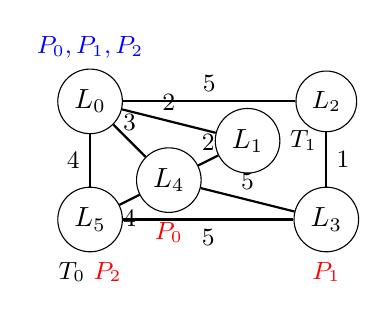
\begin{tikzpicture}[scale=0.5]
  \node[draw, circle, label=above:{\small \textcolor{blue}{$P_0, P_1,P_2$}}] (l0) at (0,0) {$L_0$};
  \node[draw, circle, label=right:{\small $T_1$}] (l1) at (4,-1) {$L_1$};
  \node[draw, circle] (l2) at (6,0) {\small $L_2$};
  \node[draw, circle, label=below:{\small \textcolor{red}{$P_1$}}] (l3) at (6,-3) {$L_3$};
  \node[draw, circle, label=below:{\small \textcolor{red}{$P_0$}}] (l4) at (2,-2) {$L_4$};
  \node[draw, circle, label=below:{\small $T_0$ \textcolor{red}{$P_2$}}] (l5) at (0,-3) {$L_5$};

  \draw[thick] (l0) to node[above] {\small 5} (l2);
  \draw[thick] (l0) to node[above] {\small 2} (l1);
  \draw[thick] (l0) to node[above] {\small 3} (l4);
  \draw[thick] (l0) to node[left] {\small 4} (l5);
  \draw[thick] (l2) to node[right] {\small 1} (l3);
  \draw[thick] (l4) to node[above] {\small 2} (l1);
  \draw[thick] (l4) to node[above] {\small 5} (l3);
  \draw[thick] (l5) to node[below] {\small 5} (l3);
  \draw[thick] (l4) to node[below] {\small 4} (l5);
\end{tikzpicture}
\vspace{-0.2cm}
\hspace{-0.6cm} \caption{Illustrative IPC NoMystery example.}
\label{fig:nomystery-example}
\vspace{-0.2cm}
\end{wrapfigure}

We define three kinds of action-set properties for this domain:
\emph{uses $T_i$ $(L_x,L_y)$} (truck $T_i$ drives at least once from
$L_x$ to $L_y$ or vice versa); \emph{doesn't use $T_i$ $(L_x,L_y)$}
(truck $T_i$ does not drive from $L_x$ to $L_y$ or vice versa);
\emph{same truck $P_x$ $P_y$} (both packages are delivered by the same
truck). We consider six instances of these properties: 1.\ uses $T_0$
$(L_2,L_3)$; 2.\ same truck $P_1$ $P_2$; 3.\ uses $T_0$ $(L_4,L_3)$;
4.\ same truck $P_2$ $P_0$; 5.\ doesn't use $T_0$ $(L_0,L_5)$;
6.\ uses $T_1$ $(L_5,L_4)$.

Fixing the package destinations as hard goals (defining the set of
plans \plans\ considered), and computing the MUGS over these six
action-set properties using the algorithms previously described, it
turns out there are 7 minimal unsolvable subsets of these properties,
each of size 3.

Say now that the current plan uses $T_0$ only, and includes the action
(drive T0 L5 L0). The user might ask \emph{''Why don't you avoid the
  road $L_0-L_5$, which has a lot of traffic at the
  moment?''}. Answering this question in terms of contrastive
explanation, as previously discussed, corresponds to forcing property
5 to be satisfied. At the same time, the plan already satisfies
properties 2 and 4. However, one of the MUGS is $\{2,4,5\}$, and hence
the answer to the user question would be: \textit{Because if you don't
  use that road, then you would not be able to deliver all packages
  using a single truck}.


%!TEX root=./main.tex


% pgf settings: shrink the tick labels a bit
\pgfplotsset{every tick label/.append style={font=\scriptsize}}

\newcommand{\scatterplotsize}{8cm}
\newcommand{\scatterplotxlabelshift}{1.5ex}
\newcommand{\scatterplotylabelshift}{-3ex}

\section{Experiments}

\joerg{tentative plan, to simplify presentation and focus on the 
main messages rather than algorothm-configuration space: use hFF
throughout, and vary SysW (aka top-down) vs SysS (aka bottom-up)
throughout; on IPC benchmarks, vary hC on vs off, where ``on'' means
to include transfer; on action-set prop experiments, vary traps on vs
off, where ``on'' means to include transfer. ... Rebecca to generate
the missing data for IPC and nomystery, then we'll check and if it
looks ok use this.}

\rebecca{ 1-1.5 page(s) Michael/Rebecca }


\joerg{Ideally, we should actually do something with existing oversubscription 
	planning benchmarks. Carmel and Mirkis generated ones in their
	work
	(http://iew3.technion.ac.il/~dcarmel/Papers/Sources/ecai14b.pdf),
	from IPC benchmarks, by restricting plan cost to 25\%, 50\%,
	75\%, and 100\% of optimal plan cost for all goals. Emulate
	this, for unit action costs, in a way that makes our current
	technology applicable.}



\setlength{\tabcolsep}{2pt}
\renewcommand{\arraystretch}{0.8}
\begin{figure*}[ht]
	\centering 	\scriptsize
	\begin{tabular}{l|rr|rr|rr|rr||rr|rr|rr|rr||rr|rr|rr|rr}
		& \multicolumn{8}{c}{0.25} & \multicolumn{8}{c}{0.5} & \multicolumn{8}{c}{0.75}\\
		& \multicolumn{2}{c}{C} & \multicolumn{2}{c}{Cnr} & \multicolumn{2}{c}{max} & & & \multicolumn{2}{c}{C} & \multicolumn{2}{c}{Cnr} & \multicolumn{2}{c}{max} & & &  \multicolumn{2}{c}{C} & \multicolumn{2}{c}{Cnr} & \multicolumn{2}{c}{max} & &\\\hline
		& c & t & c & t & c & t & nodes & mugs & c & t & c & t & c & t & nodes & mugs &  c & t & c & t & c & t & nodes & mugs\\\hline
		airport (28) & 0.79 & 0.0017 & 0.79 & 0.0066 & 0.86 & 18.3645 & 7 & 2.05 & 0.54 & 3.5596 & 0.54 & 3.5753 & 0.68 & 3.769 & 5 & 1.47 & 0.29 & 0.0078 & 0.29 & 0.0079 & 0.68 & 0.0035 & 3 & 1\\
		barman (4) & 1 & 0.0047 & 1 & 0.0144 & 1 & 0.0563 & 9 & 3 & 1 & 52.8352 & 1 & 43.8564 & 1 & 8.1814 & 8 & 3 & 0 & - & 0 & - & 1 & - & - & -\\
		blocks (28) & 1 & 0.0001 & 0.93 & 0.0007 & 0.96 & 0.0077 & 393 & 5.69 & 0.96 & 0.0006 & 0.93 & 0.004 & 0.75 & 0.56 & 140 & 6.05 & 0.89 & 0.0077 & 0.86 & 0.0159 & 0.61 & 1.447 & 52 & 6.06\\
		data-network (12) & 0 & - & 0 & - & 1 & - & - & - & 0 & - & 0 & - & 1 & - & - & - & 0 & - & 0 & - & 1 & - & - & -\\
		depot (7) & 1 & 0.0008 & 1 & 0.0043 & 1 & 0.1156 & 38 & 3.71 & 1 & 1.7631 & 1 & 0.7123 & 1 & 10.9838 & 36 & 6.71 & 0.43 & 6.5403 & 0.43 & 1.5582 & 0.57 & 5.8422 & 12 & 2.67\\
		driverlog (13) & 1 & 0.0002 & 1 & 0.0013 & 1 & 0.0432 & 556 & 6.38 & 0.92 & 0.0137 & 0.92 & 0.0374 & 0.77 & 0.3713 & 388 & 13.4 & 0.69 & 3.2144 & 0.69 & 1.9891 & 0.62 & 9.1767 & 191 & 7.88\\
		elevators (40) & 0 & - & 0 & - & 1 & - & - & - & 0 & - & 0 & - & 1 & - & - & - & 0 & - & 0 & - & 0.83 & - & - & -\\
		floortile (13) & 0 & - & 0 & - & 0.46 & - & - & - & 0 & - & 0 & - & 0.15 & - & - & - & 0 & - & 0 & - & 0.15 & - & - & -\\
		freecell (15) & 1 & 0.0003 & 1 & 0.0054 & 1 & 0.15 & 17 & 4 & 0.4 & 0.0085 & 0.47 & 0.0175 & 1 & 0.1357 & 16 & 5.2 & 0 & - & 0 & - & 0.93 & - & - & -\\
		ged (15) & 0 & - & 0 & - & 0.67 & - & - & - & 0 & - & 0 & - & 0.67 & - & - & - & 0 & - & 0 & - & 0.67 & - & - & -\\
		grid (2) & 1 & 0.0002 & 1 & 0.0034 & 1 & 0.0138 & 6 & 1.5 & 1 & 0.0122 & 1 & 0.0177 & 1 & 1.2066 & 6 & 1.5 & 0.5 & 0.0018 & 1 & 0.004 & 1 & 0.02 & 3 & 1\\
		gripper (7) & 0.71 & 0.0079 & 0.71 & 0.0069 & 0.71 & 0.0172 & 1087 & 77.4 & 0.57 & 1.0907 & 0.57 & 0.1444 & 0.57 & 0.0733 & 286 & 87 & 0.43 & 1.4578 & 0.43 & 0.8578 & 0.71 & 0.0336 & 43 & 12.67\\
		hiking (9) & 1 & 0.0019 & 1 & 0.0029 & 1 & 0.1407 & 4 & 1.44 & 0.67 & 0.4672 & 0.67 & 0.3678 & 1 & 3.9923 & 4 & 1.67 & 0.22 & 2.5099 & 0.22 & 1.1453 & 1 & 0.9072 & 4 & 1\\
		logistics (26) & 1 & 0.0007 & 1 & 0.0036 & 0.85 & 4.5539 & 110 & 4.05 & 0.77 & 0.1136 & 0.85 & 0.0671 & 0.58 & 5.1033 & 48 & 4.53 & 0.54 & 0.3488 & 0.58 & 0.1775 & 0.46 & 0.2939 & 22 & 2.17\\
		miconic (141) & 0.47 & 0.0016 & 0.46 & 0.0044 & 0.4 & 0.0477 & 438 & 27.89 & 0.29 & 0.3027 & 0.35 & 0.0338 & 0.32 & 0.1269 & 66 & 17.78 & 0.25 & 0.9975 & 0.28 & 0.1975 & 0.32 & 0.091 & 20 & 5.54\\
		mprime (22) & 1 & 0.0002 & 1 & 0.0036 & 1 & 0.0115 & 4 & 1.32 & 1 & 0.0011 & 1 & 0.0044 & 1 & 0.3336 & 4 & 1.23 & 1 & 0.0167 & 1 & 0.026 & 1 & 16.9777 & 4 & 1.18\\
		mystery (17) & 1 & 0.0003 & 1 & 0.0052 & 1 & 0.0199 & 4 & 1.41 & 1 & 0.0018 & 1 & 0.0062 & 1 & 1.6016 & 4 & 1.35 & 0.82 & 0.0049 & 0.82 & 0.0134 & 0.88 & 1.513 & 4 & 1.15\\
		nomystery (14) & 0.71 & 0.0003 & 0.71 & 3 & 1 & 0.0321 & 76 & 5.4 & 0 & - & 0.07 & - & 0.71 & - & - & - & 0 & - & 0 & - & 0.57 & - & - & -\\
		openstacks (47) & 0.15 & 0.0016 & 0.15 & 24 & 0.51 & 0.1372 & 316 & 6.43 & 0.11 & 0.0177 & 0.11 & 0.0372 & 0.47 & 0.0163 & 33 & 4.2 & 0.11 & - & 0 & - & 0.43 & - & - & -\\
		org-syn (7) & 1 & 0.0002 & 0.86 & 0.0179 & 0.86 & 0.0486 & 40 & 3.17 & 1 & 0.0011 & 0.86 & 0.0198 & 0.86 & 0.0504 & 40 & 3.17 & 1 & 0.0013 & 0.86 & 0.0208 & 0.86 & 0.054 & 40 & 3.17\\
		org-syn-s (10) & 0.8 & 0.0007 & 0.6 & 0.0152 & 0.6 & 5.9967 & 64 & 3.17 & 0.5 & 0.0004 & 0.5 & 0.0062 & 0.6 & 0.0374 & 70 & 3 & 0.2 & 0.0003 & 0.2 & 0.0072 & 0.6 & 0.0293 & 129 & 6\\
		parcprinter (24) & 0 & - & 0 & - & 0.42 & - & - & - & 0 & - & 0 & - & 0.42 & - & - & - & 0 & - & 0 & - & 0.42 & - & - & -\\
		parking (5) & 1 & - & 0 & - & 0 & - & - & - & 0.2 & - & 0 & - & 0 & - & - & - & 0 & - & 0 & - & 0 & - & - & -\\
		pathways-noneg (5) & 1 & 0.0002 & 1 & 0.0009 & 1 & 1.5975 & 20 & 3.2 & 0.4 & 0.0002 & 0.4 & 0.0002 & 0.8 & 0.0043 & 4 & 1.5 & 0.2 & 0.0001 & 0.2 & 0.0002 & 0.8 & 0.0022 & 3 & 1\\
		pegsol (2) & 0 & - & 0 & - & 0 & - &  &  & 0 & - & 0 & - & 0 & - & - & - & 0 & - & 0 & - & 0 & - & - & -\\
		pipesworld-nt (17) & 1 & 0.0006 & 1 & 4 & 1 & 0.0336 & 40 & 3.35 & 0.94 & 0.5306 & 0.94 & 0.3581 & 0.94 & 1.7601 & 26 & 5 & 0.82 & 10.0899 & 0.82 & 13.0619 & 0.94 & 41.5442 & 18 & 4.14\\
		pipesworld-t (12) & 0.92 & 0.0003 & 0.92 & 4 & 1 & 0.0809 & 34 & 3.45 & 0.92 & 0.2643 & 0.92 & 0.2918 & 0.92 & 11.8348 & 31 & 5 & 0.75 & 0.4525 & 0.75 & 0.6277 & 0.75 & 18.627 & 15 & 3.13\\
		psr-small (49) & 1 & 0.0002 & 0.98 & 0.0007 & 0.98 & 0.0006 & 615 & 3.44 & 1 & 0.0009 & 0.98 & 0.0035 & 0.98 & 0.004 & 475 & 2.52 & 0.96 & 0.0055 & 0.92 & 0.0135 & 0.96 & 0.0637 & 83 & 1.78\\
		rovers (8) & 1 & 0.0097 & 1 & 0.0031 & 1 & 0.0873 & 163 & 18 & 0.88 & 0.6903 & 0.88 & 0.0918 & 0.88 & 1.8094 & 34 & 11.43 & 0.5 & 0.0016 & 0.88 & 0.0018 & 0.75 & 0.0024 & 6 & 1.5\\
		satellite (7) & 1 & 0.0002 & 1 & 0.0027 & 1 & 0.3211 & 176 & 5.57 & 0.86 & 0.0417 & 1 & 0.0461 & 0.86 & 1.2065 & 114 & 18.67 & 0.71 & 0.2023 & 0.86 & 0.1006 & 0.57 & 0.1612 & 51 & 13.25\\
		scanalyzer (23) & 0.57 & 0.0001 & 0.39 & 0.0012 & 0.39 & 0.0103 & 2359 & 12.67 & 0.39 & 0.0476 & 0.39 & 0.0198 & 0.39 & 0.1573 & 1939 & 45.78 & 0.22 & 0.131 & 0.22 & 0.0369 & 0.39 & 0.1435 & 550 & 30.8\\
		snake (7) & 0.57 & 0.0008 & 0.14 & 0.0151 & 0.14 & 0.1996 & 245 & 4 & 0 & - & 0 & - & 0.14 & - & - & - & 0 & - & 0 & - & 0.14 & - & - & -\\
		sokoban (50) & 0 & - & 0 & - & 0.98 & - & - & - & 0 & - & 0 & - & 0.94 & - & - & - & 0 & - & 0 & - & 0.84 & - & - & -\\
		storage (15) & 1 & 0.0003 & 1 & 1 & 1 & 0.0025 & 13 & 3.6 & 1 & 0.2554 & 1 & 0.0665 & 1 & 0.1762 & 11 & 3.73 & 0.93 & 9.902 & 0.93 & 3.744 & 1 & 0.9675 & 7 & 1.93\\
		termes (6) & 1 & 0.0008 & 0.33 & 0.0469 & 1 & 36 & 2881 & 2.5 & 0.17 & - & 0 & - & 0.17 & - & - & - & 0 & - & 0 &  & 0 & - & - & -\\
		tetris (6) & 0.83 & 0.0003 & 0.33 & 0.0088 & 0.33 & 0.0147 & 257 & 6.5 & 0.5 & 0.0133 & 0.33 & 0.0297 & 0.33 & 0.0307 & 205 & 10 & 0.33 & 0.8305 & 0.33 & 0.5429 & 0.5 & 0.1313 & 106 & 5.5\\
		tidybot (23) & 1 & 0.0032 & 1 & 0.0536 & 1 & 1.4659 & 16 & 2.57 & 0.7 & 3.9946 & 0.7 & 3.3744 & 1 & 34.3564 & 16 & 3 & 0.43 & 7.1982 & 0.3 & 10.1166 & 0.3 & 14.7701 & 15 & 3.5\\
		tpp (7) & 1 & 0.0002 & 1 & 1 & 1 & 24 & 37 & 3.86 & 1 & 0.0328 & 1 & 0.0201 & 0.86 & 0.2812 & 21 & 6.17 & 0.71 & 0.0469 & 0.86 & 0.0242 & 0.86 & 0.014 & 9 & 2.8\\
		transport (23) & 1 & 0.0004 & 1 & 0.0015 & 1 & 0.0154 & 17 & 3.04 & 1 & 0.0649 & 1 & 0.1057 & 1 & 1.0104 & 16 & 3.17 & 0.96 & 6.7547 & 0.96 & 4.1551 & 1 & 14.8687 & 12 & 2.05\\
		trucks (10) & 0.2 & 0.0001 & 0.2 & 0.0003 & 1 & 0.0012 & 13 & 3.5 & 0 & - & 0 & - & 0.6 & - & - & - & 0 & - & 0 & - & 0.6 & - & - & -\\
		visitall (14) & 0.71 & 0.0001 & 0.57 & 0.0002 & 0.64 & 0.0004 & 10292 & 19.88 & 0.71 & 0.0002 & 0.5 & 0.0013 & 0.57 & 0.0046 & 6930 & 38 & 0.57 & 0.0034 & 0.5 & 0.0087 & 0.5 & 0.0338 & 4533 & 38.29\\
		woodworking (29) & 0.45 & 0.0001 & 0.17 & 0.0006 & 0.24 & 0.0016 & 2148 & 17.8 & 0.1 & 0.0012 & 0.1 & 0.0058 & 0.17 & 0.0134 & 1426 & 29 & 0.07 & 0.0097 & 0.1 & 0.0802 & 0.17 & 0.1136 & 1093 & 17\\
		zenotravel (13) & 1 & 0.0008 & 1 & 0.0073 & 0.92 & 0.2413 & 122 & 8 & 0.69 & 0.0011 & 0.77 & 0.0045 & 0.62 & 0.0424 & 38 & 3.75 & 0.69 & 0.4634 & 0.69 & 0.3243 & 0.62 & 1.6294 & 26 & 2.38\\\hline
		(862) & 0.62 & 0.0012 & 0.58 & 0.0077 & 0.76 & 0.9414 & 632 & 8.05 & 0.48 & 2.0666 & 0.49 & 1.6665 & 0.68 & 2.7886 & 392 & 11.97 & 0.39 & 1.7662 & 0.39 & 1.3409 & 0.62 & 4.4643 & 245 & 6.95\\
	\end{tabular}

 
	\caption{
		Benchmark: oversubscription IPC
		domains with bound $ = x \cdot $ optimal cost with $
		x \in \{0.25, 0.5, 0.75\}$, solvable with lmcut with no cost bound in 
		30 min and with less then 31 goal facts(limitation of implementation).
		hff: $h^{FF}$ with gready-best-first-search and preferred operators and 
		bottom-up meta search; maxbu: $h^{max}$ with $A^*$ and bottom-up meta search;
		maxtd: $h^{max}$ with $A^*$ and top-down meta search; hC(p): online learned
		dead-end detectors with bounded DFS with and without propagation of the
		learn detectors through the top-down meta search three.
	}
\end{figure*}


\begin{figure*}[ht]
	\centering \tiny
% 3 * 5 coverage, 3 * goal size, 3 * 2 fraction search tree
\begin{tabular}{l|rr:rr|rr:rr|rr:rr}
	domain & \multicolumn{4}{c|}{0.25} & \multicolumn{4}{c|}{0.5} & \multicolumn{4}{c|}{0.75}  \\\hline
	&  hff bu & hC bu & hff td & hC td & hff bu & hC bu & hff td & hC td & hff bu & hC bu & hff td & hC td\\\hline
	airport (28) & 25 & 26 & 24 & \textbf{27}  & 19 & \textbf{21}  & 19 & \textbf{21}  & \textbf{19}  & 16 & \textbf{19}  & 16\\
	barman (4) & 4 & 4 & 4 & 4 & 4 & 4 & 4 & 4 & \textbf{4}  & 0 & \textbf{4}  & \textbf{4} \\
	blocks (28) & \textbf{28}  & \textbf{28}  & 27 & \textbf{28}  & 23 & \textbf{27}  & 21 & \textbf{27}  & 18 & 24 & 17 & \textbf{26} \\
	data-network (12) & 12 & 12 & 12 & 12 & 12 & 12 & 12 & 12 & 11 & \textbf{12}  & 11 & \textbf{12} \\
	depot (7) & 7 & 7 & 7 & 7 & 7 & 7 & 7 & 7 & \textbf{4}  & 3 & \textbf{4}  & 3\\
	driverlog (13) & 13 & 13 & 13 & 13 & 10 & 11 & 10 & \textbf{12}  & \textbf{8}  & 10 & 7 & 10\\
	elevators (40) & 40 & 40 & 40 & 40 & \textbf{40}  & 37 & 38 & 37 & \textbf{35}  & 26 & 31 & 26\\
	floortile (13) & 7 & 7 & 6 & \textbf{8}  & 2 & 2 & 2 & 2 & \textbf{2}  & 1 & \textbf{2}  & \textbf{2} \\
	freecell (15) & 15 & 15 & 15 & 15 & 15 & 15 & 15 & 15 & \textbf{14}  & 13 & 13 & 13\\
	ged (15) & 15 & 15 & 15 & 15 & \textbf{15}  & 10 & 10 & 10 & 10 & \textbf{7}  & 10 & \textbf{7} \\
	grid (2) & 2 & 2 & 2 & 2 & 2 & 2 & 2 & 2 & 2 & 2 & 2 & 2\\
	gripper (7) & \textbf{7}  & 5 & 5 & 5 & 4 & 4 & 4 & 4 & \textbf{4}  & 3 & \textbf{4}  & 3\\
	hiking (9) & 9 & 9 & 9 & 9 & 9 & 9 & 9 & 9 & 9 & 9 & 9 & 9\\
	logistics (26) & 24 & \textbf{26}  & 21 & \textbf{26}  & 15 & 19 & 14 & \textbf{20}  & 12 & 13 & 12 & \textbf{15} \\
	miconic (141) & \textbf{66}  & \textbf{66}  & 55 & 64 & \textbf{45}  & 40 & 44 & 43 & \textbf{41}  & 36 & 40 & 36\\
	movie (30) & 30 & 30 & 30 & 30 & 30 & 30 & 30 & 30 & 30 & 30 & 30 & 30\\
	mprime (22) & 22 & 22 & 22 & 22 & 22 & 22 & 22 & 22 & 22 & 22 & 22 & 22\\
	mystery (17) & 17 & 17 & 17 & 17 & 17 & 17 & 17 & 17 & 15 & \textbf{17}  & 15 & \textbf{17} \\
	nomystery (14) & 14 & 14 & 14 & 14 & 10 & \textbf{12}  & 10 & \textbf{12}  & 8 & 8 & 8 & 8\\
	openstacks (47) & \textbf{45}  & \textbf{45}  & 37 & 43 & \textbf{45}  & 43 & 29 & 41 & \textbf{42}  & \textbf{42}  & 22 & 33\\
	organic-synthesis (7) & 7 & 7 & 7 & 7 & 7 & 7 & 7 & 7 & 7 & 7 & 7 & 7\\
	organic-synthesis-split (10) & \textbf{8}  & \textbf{8}  & 7 & \textbf{8}  & \textbf{8}  & \textbf{8}  & 7 & \textbf{8}  & \textbf{7}  & 6 & 6 & 6\\
	parcprinter (24) & 10 & 10 & 10 & \textbf{14}  & 10 & 10 & 10 & \textbf{14}  & 10 & 10 & 10 & \textbf{12} \\
	parking (5) & \textbf{5}  & \textbf{5}  & 4 & \textbf{5}  & 0 & \textbf{1}  & 0 & \textbf{1}  & 0 & 0 & 0 & 0\\
	pathways-noneg (5) & 5 & 5 & 5 & 5 & 4 & \textbf{5}  & 4 & \textbf{5}  & 4 & 4 & 4 & 4\\
	pegsol (2) & 0 & 0 & \textbf{2}  & \textbf{2}  & 0 & 0 & \textbf{2}  & \textbf{2}  & 0 & 0 & \textbf{2}  & \textbf{2} \\
	pipesworld-nt (17) & 17 & 17 & 17 & 17 & \textbf{17}  & \textbf{17}  & 16 & \textbf{17}  & \textbf{16}  & 14 & \textbf{16}  & 14\\
	pipesworld-t (12) & 12 & 12 & 12 & 12 & 11 & 11 & 11 & 11 & \textbf{9}  & 11 & \textbf{9}  & 10\\
	psr-small (49) & 48 & 48 & \textbf{49}  & \textbf{49}  & 47 & 47 & 48 & \textbf{49}  & 46 & 46 & \textbf{48}  & \textbf{48} \\
	rovers (8) & 8 & 8 & 8 & 8 & 7 & 7 & 7 & 7 & \textbf{6}  & 5 & \textbf{6}  & 4\\
	satellite (7) & 7 & 7 & 7 & 7 & 6 & 6 & 6 & \textbf{7}  & 4 & 5 & 4 & \textbf{6} \\
	scanalyzer (23) & \textbf{9}  & 15 & \textbf{9}  & 13 & 9 & 9 & 9 & 9 & \textbf{9}  & 5 & \textbf{9}  & \textbf{9} \\
	snake (7) & 6 & 6 & 6 & 6 & 3 & 3 & 3 & 3 & \textbf{3}  & 1 & 2 & 1\\
	sokoban (50) & \textbf{50}  & \textbf{50}  & 49 & \textbf{50}  & \textbf{46}  & 43 & 45 & 43 & \textbf{40}  & 30 & \textbf{40}  & 28\\
	storage (15) & 15 & 15 & 15 & 15 & 15 & 15 & 15 & 15 & \textbf{15}  & 14 & \textbf{15}  & 14\\
	termes (6) & \textbf{6}  & \textbf{6}  & 5 & \textbf{6}  & \textbf{5}  & 1 & 1 & 2 & \textbf{1}  & 0 & 0 & 0\\
	tetris (6) & \textbf{6}  & \textbf{6}  & 5 & \textbf{6}  & \textbf{4}  & 3 & 3 & 3 & \textbf{3}  & 2 & \textbf{3}  & 2\\
	tidybot (23) & 23 & 23 & 23 & 23 & \textbf{23}  & 22 & \textbf{23}  & 22 & 13 & 13 & \textbf{7}  & 14\\
	tpp (7) & 7 & 7 & 7 & 7 & 6 & \textbf{7}  & 6 & 6 & \textbf{6}  & 5 & \textbf{6}  & 5\\
	transport (23) & 23 & 23 & 23 & 23 & 23 & 23 & 23 & 23 & \textbf{23}  & 22 & 22 & 22\\
	trucks (10) & 10 & 10 & \textbf{9}  & 10 & 6 & \textbf{7}  & 6 & \textbf{7}  & \textbf{5}  & 3 & \textbf{5}  & 4\\
	visitall (14) & \textbf{13}  & \textbf{13}  & 10 & 10 & \textbf{9}  & 10 & 8 & 10 & 6 & 6 & 7 & \textbf{8} \\
	woodworking (29) & \textbf{23}  & \textbf{23}  & 12 & 15 & \textbf{9}  & \textbf{9}  & 5 & \textbf{9}  & 5 & 5 & 5 & 5\\
	zenotravel (13) & \textbf{13}  & \textbf{13}  & 12 & \textbf{13}  & \textbf{9}  & \textbf{9}  & 8 & \textbf{9}  & 8 & \textbf{9}  & 8 & \textbf{9} \\\hline
	Sum (862) & 733 & \textbf{740}  & 688 & 732 & 630 & 624 & 592 & \textbf{636}  & \textbf{556}  & 517 & 523 & 528\\
\end{tabular}
 
	\caption{
		Benchmark: oversubscription IPC
		domains with bound $ = x \cdot $ optimal cost with $
		x \in \{0.25, 0.5, 0.75\}$, solvable with lmcut with no cost bound in 
		30 min and with less then 31 goal facts(limitation of implementation).
	}
\end{figure*}

\begin{figure}[ht]
\scriptsize
\begin{subfigure}[t]{0.22\textwidth}
\begin{tikzpicture}
	\begin{axis}
		 [
			grid,
			width=4.5cm,
			height=4.5cm,
			log origin = 0,
			% ymode = log,
			xtick = {0.25,0.5,0.75},
			legend style={at={(0.95,-0.15)}},
			legend columns=2,
			ybar,
			bar width=2pt,
			enlarge x limits=0.3,
		 ]
		\addplot+[blue] coordinates
			{(0.25, 0.48) (0.5, 1.44) (0.75, 4.02)};
		\addplot+[red] coordinates
			{(0.25, 0.0099) (0.5, 1.34) (0.75, 3.02)};
		\addplot+[yellow] coordinates
			{(0.25, 0.53) (0.5, 2.22) (0.75, 6.87)};
		\addplot+[darkgreen] coordinates
			{(0.25, 0.0038) (0.5, 1.06) (0.75, 4.26)};
		\legend{hff bu, hC hff bu, hff td, hC hff td}
	\end{axis}
\end{tikzpicture}
\caption{}
\label{fig:avg-search-time}
\end{subfigure}
\begin{subfigure}[t]{0.22\textwidth}
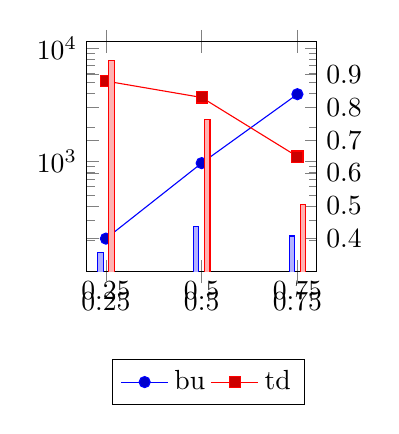
\begin{tikzpicture}
	\begin{axis}
		 [
			width=4.5cm,
			height=4.5cm,
			ymin= 0.3,
			ymax = 1,
			%grid,
			%ymode = log,
			xtick = {0.25,0.5,0.75},
			ytick = {0.4,0.5,0.6,0.7,0.8,0.9},
			%yticklabels = {0.1,0.2,0.3,0.4,0.5,0.6,0.7,0.8,0.9,1.0},
			legend style={at={(0.95,-0.38)}},
			legend columns=4,
			yticklabel pos=right
		 ]
		\addplot+[sharp plot] coordinates
			{(0.25, 0.40) (0.5, 0.63) (0.75, 0.84)};
		\addplot+[sharp plot] coordinates
			{(0.25, 0.88) (0.5, 0.83) (0.75, 0.65)};
		\legend{bu, td}
	\end{axis}
	\begin{axis}
		 [
			width=4.5cm,
			height=4.5cm,
			%grid,
			ymode = log,
			xtick = {0.25,0.5,0.75},
			ytick = {10,100,1000,10000},
			%yticklabels = {0.1,0.2,0.3,0.4,0.5,0.6,0.7,0.8,0.9,1.0},
			legend style={at={(0.95,-0.38)}},
			legend columns=4,
			yticklabel pos=left,
			ybar,
			bar width=2pt,
		 ]
		\addplot+[] coordinates
			{(0.25, 158) (0.5, 268) (0.75, 220)};
		\addplot+[] coordinates
			{(0.25, 7735) (0.5, 2337) (0.75, 415)};
	\end{axis}
\end{tikzpicture}
\caption{}
\label{fig:frac-meta-search-tree}
\end{subfigure}
\caption{(a) average search time per meta search node; 
	(b) average fraction of explored meta search tree} 
\end{figure}



\subsubsection*{Action Set Properties}


\FloatBarrier
\begin{figure*}[ht]

\tiny
\begin{tikzpicture}


\begin{axis}[
width = 7cm,
height=4cm,
enlarge x limits = 0.1,
enlarge y limits = 0.1,
ybar,
bar width=1pt,
ymin = 0,
ymax = 10,
at={(0.0\linewidth,-0.0)},
compat=1.6,
title=c 100,
ylabel=goals 4,
]
\addplot+[ybar, bar shift =-6pt, gray,
]
plot coordinates {
(07, 10)
(08, 10)
(01, 10)
(09, 10)
(06, 10)
(03, 10)
(04, 10)
(05, 10)
(02, 10)
(10, 9)
};
\label{plot:properties_hff_bu}
\addplot+[ybar, bar shift =-3pt, blue,
]
plot coordinates {
(07, 10)
(05, 10)
(04, 10)
(08, 10)
(01, 10)
(09, 10)
(03, 10)
(06, 10)
(02, 10)
(10, 10)
};
\label{plot:properties_hmax_bu}
\addplot+[ybar, bar shift =-4.5pt, purple,
]
plot coordinates {
(07, 10)
(04, 10)
(08, 10)
(09, 9)
(03, 10)
(06, 10)
(05, 10)
(01, 10)
(10, 9)
(02, 10)
};
\label{plot:properties_hmax_td}
\addplot+[ybar, bar shift =-1.5pt, yellow,
]
plot coordinates {
(05, 10)
(08, 10)
(07, 10)
(09, 10)
(03, 10)
(04, 10)
(06, 10)
(01, 10)
(10, 10)
(02, 10)
};
\label{plot:properties_trap_bu}
\addplot+[ybar, bar shift =0pt, orange,
]
plot coordinates {
(04, 10)
(08, 10)
(01, 10)
(09, 10)
(06, 10)
(03, 10)
(07, 10)
(05, 10)
(02, 10)
(10, 10)
};
\label{plot:properties_trap_td}
\addplot+[ybar, bar shift =1.5pt, red,
]
plot coordinates {
(07, 7)
(08, 9)
(09, 6)
(03, 10)
(06, 7)
(04, 9)
(05, 8)
(01, 10)
(10, 5)
(02, 10)
};
\label{plot:properties_hC_td}
\addplot+[ybar, bar shift =3pt, darkgreen,
]
plot coordinates {
(07, 5)
(05, 8)
(04, 10)
(08, 4)
(09, 2)
(03, 10)
(06, 5)
(01, 10)
(02, 10)
(10, 0)
};
\label{plot:properties_hCnr_td}

\end{axis}
\hfill


\begin{axis}[
width = 7cm,
height=4cm,
enlarge x limits = 0.1,
enlarge y limits = 0.1,
ybar,
bar width=1pt,
ymin = 0,
ymax = 10,
at={(0.333333333333\linewidth,-0.0)},
compat=1.6,
title=c 150,
]
\addplot+[ybar, bar shift =-6pt, gray,
]
plot coordinates {
(05, 9)
(04, 10)
(03, 10)
(10, 1)
(02, 10)
(06, 8)
(09, 1)
(08, 2)
(07, 5)
(01, 10)
};
\label{plot:properties_hff_bu}
\addplot+[ybar, bar shift =-3pt, blue,
]
plot coordinates {
(05, 7)
(04, 10)
(03, 10)
(10, 0)
(02, 10)
(08, 1)
(07, 2)
(06, 3)
(01, 10)
(09, 1)
};
\label{plot:properties_hmax_bu}
\addplot+[ybar, bar shift =-4.5pt, purple,
]
plot coordinates {
(05, 9)
(04, 10)
(03, 10)
(10, 0)
(02, 10)
(08, 1)
(07, 3)
(09, 1)
(06, 7)
(01, 10)
};
\label{plot:properties_hmax_td}
\addplot+[ybar, bar shift =-1.5pt, yellow,
]
plot coordinates {
(05, 8)
(04, 9)
(10, 2)
(02, 10)
(09, 2)
(08, 3)
(03, 10)
(07, 5)
(06, 6)
(01, 10)
};
\label{plot:properties_trap_bu}
\addplot+[ybar, bar shift =0pt, orange,
]
plot coordinates {
(05, 10)
(08, 4)
(04, 10)
(03, 10)
(10, 2)
(02, 10)
(06, 8)
(07, 4)
(01, 10)
(09, 3)
};
\label{plot:properties_trap_td}
\addplot+[ybar, bar shift =1.5pt, red,
]
plot coordinates {
(05, 3)
(08, 0)
(04, 5)
(10, 0)
(02, 8)
(03, 5)
(07, 0)
(09, 0)
(06, 1)
(01, 10)
};
\label{plot:properties_hC_td}
\addplot+[ybar, bar shift =3pt, darkgreen,
]
plot coordinates {
(05, 3)
(04, 5)
(10, 0)
(02, 8)
(09, 0)
(08, 0)
(03, 6)
(07, 0)
(06, 0)
(01, 10)
};
\label{plot:properties_hCnr_td}

\end{axis}
\hfill


\begin{axis}[
width = 7cm,
height=4cm,
enlarge x limits = 0.1,
enlarge y limits = 0.1,
ybar,
bar width=1pt,
ymin = 0,
ymax = 10,
at={(0.666666666667\linewidth,-0.0)},
compat=1.6,
title=c 200,
]
\addplot+[ybar, bar shift =-6pt, gray,
]
plot coordinates {
(08, 1)
(02, 10)
(03, 10)
(04, 10)
(07, 2)
(09, 0)
(01, 10)
(06, 6)
(10, 0)
(05, 10)
};
\label{plot:properties_hff_bu}
\addplot+[ybar, bar shift =-3pt, blue,
]
plot coordinates {
(08, 0)
(04, 3)
(01, 10)
(07, 0)
(10, 0)
(03, 8)
(09, 0)
(02, 10)
(06, 0)
(05, 1)
};
\label{plot:properties_hmax_bu}
\addplot+[ybar, bar shift =-4.5pt, purple,
]
plot coordinates {
(08, 6)
(07, 8)
(02, 10)
(06, 9)
(04, 10)
(01, 10)
(03, 10)
(09, 5)
(05, 10)
(10, 2)
};
\label{plot:properties_hmax_td}
\addplot+[ybar, bar shift =-1.5pt, yellow,
]
plot coordinates {
(08, 2)
(07, 3)
(03, 10)
(06, 5)
(04, 10)
(09, 0)
(01, 10)
(02, 10)
(05, 9)
(10, 0)
};
\label{plot:properties_trap_bu}
\addplot+[ybar, bar shift =0pt, orange,
]
plot coordinates {
(08, 7)
(02, 10)
(04, 10)
(07, 7)
(03, 10)
(09, 6)
(01, 10)
(06, 10)
(10, 3)
(05, 10)
};
\label{plot:properties_trap_td}
\addplot+[ybar, bar shift =1.5pt, red,
]
plot coordinates {
(08, 0)
(02, 7)
(03, 3)
(06, 1)
(04, 4)
(01, 10)
(07, 0)
(10, 0)
(09, 0)
(05, 2)
};
\label{plot:properties_hC_td}
\addplot+[ybar, bar shift =3pt, darkgreen,
]
plot coordinates {
(08, 0)
(07, 0)
(06, 1)
(09, 0)
(04, 4)
(10, 0)
(03, 3)
(02, 7)
(01, 10)
(05, 2)
};
\label{plot:properties_hCnr_td}

\end{axis}
\hfill


\begin{axis}[
width = 7cm,
height=4cm,
enlarge x limits = 0.1,
enlarge y limits = 0.1,
ybar,
bar width=1pt,
ymin = 0,
ymax = 10,
at={(0.0\linewidth,-160.0)},
compat=1.6,
ylabel=goals 5,
]
\addplot+[ybar, bar shift =-6pt, gray,
]
plot coordinates {
(01, 10)
(08, 9)
(05, 10)
(03, 10)
(02, 10)
(09, 9)
(04, 10)
(07, 9)
(06, 10)
(10, 9)
};
\label{plot:properties_hff_bu}
\addplot+[ybar, bar shift =-3pt, blue,
]
plot coordinates {
(01, 10)
(08, 9)
(03, 10)
(02, 10)
(09, 9)
(07, 9)
(05, 10)
(04, 10)
(06, 10)
(10, 9)
};
\label{plot:properties_hmax_bu}
\addplot+[ybar, bar shift =-4.5pt, purple,
]
plot coordinates {
(01, 10)
(08, 6)
(03, 10)
(05, 10)
(02, 10)
(09, 6)
(04, 10)
(07, 8)
(06, 10)
(10, 2)
};
\label{plot:properties_hmax_td}
\addplot+[ybar, bar shift =-1.5pt, yellow,
]
plot coordinates {
(01, 10)
(08, 10)
(03, 10)
(02, 10)
(07, 10)
(05, 10)
(04, 10)
(09, 10)
(06, 10)
(10, 10)
};
\label{plot:properties_trap_bu}
\addplot+[ybar, bar shift =0pt, orange,
]
plot coordinates {
(01, 10)
(08, 10)
(03, 10)
(02, 10)
(09, 10)
(04, 10)
(07, 10)
(05, 10)
(06, 10)
(10, 10)
};
\label{plot:properties_trap_td}
\addplot+[ybar, bar shift =1.5pt, red,
]
plot coordinates {
(01, 10)
(08, 6)
(03, 8)
(02, 8)
(09, 5)
(04, 8)
(07, 5)
(06, 4)
(10, 2)
(05, 8)
};
\label{plot:properties_hC_td}
\addplot+[ybar, bar shift =3pt, darkgreen,
]
plot coordinates {
(01, 10)
(08, 1)
(03, 8)
(02, 8)
(09, 1)
(04, 8)
(07, 2)
(05, 6)
(06, 2)
(10, 1)
};
\label{plot:properties_hCnr_td}

\end{axis}
\hfill


\begin{axis}[
width = 7cm,
height=4cm,
enlarge x limits = 0.1,
enlarge y limits = 0.1,
ybar,
bar width=1pt,
ymin = 0,
ymax = 10,
at={(0.333333333333\linewidth,-160.0)},
compat=1.6,
]
\addplot+[ybar, bar shift =-6pt, gray,
]
plot coordinates {
(05, 5)
(06, 2)
(10, 0)
(04, 9)
(01, 10)
(09, 0)
(02, 10)
(08, 1)
(07, 1)
(03, 10)
};
\label{plot:properties_hff_bu}
\addplot+[ybar, bar shift =-3pt, blue,
]
plot coordinates {
(05, 1)
(06, 1)
(10, 0)
(03, 6)
(04, 4)
(01, 10)
(09, 0)
(02, 10)
(07, 1)
(08, 1)
};
\label{plot:properties_hmax_bu}
\addplot+[ybar, bar shift =-4.5pt, purple,
]
plot coordinates {
(05, 7)
(06, 4)
(10, 1)
(03, 10)
(04, 9)
(01, 10)
(09, 1)
(02, 10)
(07, 1)
(08, 1)
};
\label{plot:properties_hmax_td}
\addplot+[ybar, bar shift =-1.5pt, yellow,
]
plot coordinates {
(05, 6)
(06, 2)
(10, 1)
(04, 10)
(01, 10)
(09, 1)
(02, 10)
(08, 1)
(07, 1)
(03, 10)
};
\label{plot:properties_trap_bu}
\addplot+[ybar, bar shift =0pt, orange,
]
plot coordinates {
(05, 8)
(06, 4)
(10, 2)
(03, 10)
(04, 10)
(01, 10)
(09, 2)
(02, 10)
(08, 2)
(07, 2)
};
\label{plot:properties_trap_td}
\addplot+[ybar, bar shift =1.5pt, red,
]
plot coordinates {
(05, 0)
(06, 0)
(10, 0)
(03, 3)
(04, 1)
(01, 10)
(09, 0)
(02, 7)
(08, 0)
(07, 0)
};
\label{plot:properties_hC_td}
\addplot+[ybar, bar shift =3pt, darkgreen,
]
plot coordinates {
(05, 0)
(06, 0)
(10, 0)
(04, 2)
(01, 10)
(09, 0)
(02, 7)
(07, 0)
(08, 0)
(03, 4)
};
\label{plot:properties_hCnr_td}

\end{axis}
\hfill


\begin{axis}[
width = 7cm,
height=4cm,
enlarge x limits = 0.1,
enlarge y limits = 0.1,
ybar,
bar width=1pt,
ymin = 0,
ymax = 10,
at={(0.666666666667\linewidth,-160.0)},
compat=1.6,
]
\addplot+[ybar, bar shift =-6pt, gray,
]
plot coordinates {
(03, 10)
(04, 7)
(05, 3)
(09, 0)
(01, 10)
(02, 10)
(08, 0)
(06, 1)
(10, 0)
(07, 0)
};
\label{plot:properties_hff_bu}
\addplot+[ybar, bar shift =-3pt, blue,
]
plot coordinates {
(03, 1)
(04, 0)
(05, 0)
(09, 0)
(01, 8)
(02, 1)
(08, 0)
(06, 0)
(10, 0)
(07, 0)
};
\label{plot:properties_hmax_bu}
\addplot+[ybar, bar shift =-4.5pt, purple,
]
plot coordinates {
(03, 5)
(04, 3)
(05, 1)
(09, 0)
(01, 9)
(08, 0)
(02, 8)
(06, 2)
(10, 0)
(07, 1)
};
\label{plot:properties_hmax_td}
\addplot+[ybar, bar shift =-1.5pt, yellow,
]
plot coordinates {
(03, 9)
(04, 6)
(05, 1)
(09, 0)
(01, 10)
(02, 10)
(08, 0)
(06, 1)
(10, 0)
(07, 0)
};
\label{plot:properties_trap_bu}
\addplot+[ybar, bar shift =0pt, orange,
]
plot coordinates {
(03, 10)
(04, 9)
(05, 4)
(09, 2)
(01, 10)
(02, 10)
(08, 2)
(06, 4)
(10, 1)
(07, 4)
};
\label{plot:properties_trap_td}
\addplot+[ybar, bar shift =1.5pt, red,
]
plot coordinates {
(03, 2)
(04, 1)
(05, 0)
(09, 0)
(01, 10)
(08, 0)
(02, 6)
(07, 0)
(06, 0)
(10, 0)
};
\label{plot:properties_hC_td}
\addplot+[ybar, bar shift =3pt, darkgreen,
]
plot coordinates {
(03, 2)
(04, 1)
(05, 0)
(09, 0)
(01, 10)
(02, 6)
(08, 0)
(06, 0)
(10, 0)
(07, 0)
};
\label{plot:properties_hCnr_td}

\end{axis}
\hfill


\begin{axis}[
width = 7cm,
height=4cm,
enlarge x limits = 0.1,
enlarge y limits = 0.1,
ybar,
bar width=1pt,
ymin = 0,
ymax = 10,
at={(0.0\linewidth,-320.0)},
compat=1.6,
ylabel=goals 6,
]
\addplot+[ybar, bar shift =-6pt, gray,
]
plot coordinates {
(08, 2)
(09, 2)
(01, 10)
(10, 2)
(06, 5)
(04, 8)
(07, 4)
(05, 5)
(02, 9)
(03, 8)
};
\label{plot:properties_hff_bu}
\addplot+[ybar, bar shift =-3pt, blue,
]
plot coordinates {
(06, 3)
(08, 3)
(09, 2)
(01, 10)
(10, 2)
(04, 8)
(05, 5)
(07, 3)
(02, 9)
(03, 8)
};
\label{plot:properties_hmax_bu}
\addplot+[ybar, bar shift =-4.5pt, purple,
]
plot coordinates {
(08, 2)
(09, 2)
(01, 10)
(10, 2)
(06, 2)
(04, 8)
(02, 9)
(05, 5)
(07, 2)
(03, 8)
};
\label{plot:properties_hmax_td}
\addplot+[ybar, bar shift =-1.5pt, yellow,
]
plot coordinates {
(08, 8)
(09, 8)
(01, 10)
(10, 8)
(06, 9)
(04, 10)
(02, 10)
(05, 9)
(07, 8)
(03, 10)
};
\label{plot:properties_trap_bu}
\addplot+[ybar, bar shift =0pt, orange,
]
plot coordinates {
(08, 8)
(09, 8)
(01, 10)
(10, 7)
(06, 7)
(04, 8)
(07, 8)
(02, 10)
(05, 7)
(03, 8)
};
\label{plot:properties_trap_td}
\addplot+[ybar, bar shift =1.5pt, red,
]
plot coordinates {
(08, 4)
(09, 3)
(01, 10)
(10, 3)
(06, 2)
(04, 4)
(05, 3)
(07, 3)
(03, 3)
(02, 6)
};
\label{plot:properties_hC_td}
\addplot+[ybar, bar shift =3pt, darkgreen,
]
plot coordinates {
(06, 2)
(08, 1)
(09, 1)
(01, 10)
(10, 0)
(04, 3)
(05, 3)
(07, 2)
(02, 8)
(03, 3)
};
\label{plot:properties_hCnr_td}

\end{axis}
\hfill


\begin{axis}[
width = 7cm,
height=4cm,
enlarge x limits = 0.1,
enlarge y limits = 0.1,
ybar,
bar width=1pt,
ymin = 0,
ymax = 10,
at={(0.333333333333\linewidth,-320.0)},
compat=1.6,
]
\addplot+[ybar, bar shift =-6pt, gray,
]
plot coordinates {
(06, 1)
(10, 0)
(03, 9)
(05, 3)
(07, 1)
(08, 1)
(02, 10)
(09, 0)
(01, 10)
(04, 7)
};
\label{plot:properties_hff_bu}
\addplot+[ybar, bar shift =-3pt, blue,
]
plot coordinates {
(06, 0)
(10, 0)
(05, 1)
(07, 0)
(08, 0)
(02, 3)
(09, 0)
(01, 5)
(04, 2)
(03, 2)
};
\label{plot:properties_hmax_bu}
\addplot+[ybar, bar shift =-4.5pt, purple,
]
plot coordinates {
(06, 1)
(10, 0)
(03, 5)
(05, 2)
(08, 0)
(07, 0)
(02, 5)
(09, 0)
(01, 5)
(04, 3)
};
\label{plot:properties_hmax_td}
\addplot+[ybar, bar shift =-1.5pt, yellow,
]
plot coordinates {
(06, 2)
(10, 2)
(05, 2)
(08, 2)
(07, 2)
(02, 10)
(09, 2)
(01, 10)
(03, 7)
(04, 4)
};
\label{plot:properties_trap_bu}
\addplot+[ybar, bar shift =0pt, orange,
]
plot coordinates {
(06, 3)
(10, 1)
(03, 7)
(05, 3)
(08, 2)
(07, 2)
(02, 10)
(09, 2)
(01, 10)
(04, 6)
};
\label{plot:properties_trap_td}
\addplot+[ybar, bar shift =1.5pt, red,
]
plot coordinates {
(06, 0)
(10, 0)
(05, 0)
(08, 0)
(07, 0)
(02, 4)
(09, 0)
(01, 9)
(04, 0)
(03, 1)
};
\label{plot:properties_hC_td}
\addplot+[ybar, bar shift =3pt, darkgreen,
]
plot coordinates {
(06, 0)
(10, 0)
(03, 2)
(05, 0)
(07, 0)
(08, 0)
(02, 4)
(09, 0)
(01, 9)
(04, 0)
};
\label{plot:properties_hCnr_td}

\end{axis}
\hfill


\begin{axis}[
width = 7cm,
height=4cm,
enlarge x limits = 0.1,
enlarge y limits = 0.1,
ybar,
bar width=1pt,
ymin = 0,
ymax = 10,
at={(0.666666666667\linewidth,-320.0)},
compat=1.6,
]
\addplot+[ybar, bar shift =-6pt, gray,
]
plot coordinates {
(02, 8)
(01, 10)
(04, 3)
(03, 4)
(06, 1)
(10, 0)
(05, 3)
(09, 0)
(08, 0)
(07, 0)
};
\label{plot:properties_hff_bu}
\addplot+[ybar, bar shift =-3pt, blue,
]
plot coordinates {
(02, 1)
(01, 2)
(04, 0)
(03, 0)
(07, 0)
(08, 0)
(06, 0)
(10, 0)
(05, 0)
(09, 0)
};
\label{plot:properties_hmax_bu}
\addplot+[ybar, bar shift =-4.5pt, purple,
]
plot coordinates {
(02, 2)
(01, 2)
(04, 0)
(03, 1)
(08, 0)
(06, 0)
(10, 0)
(05, 0)
(09, 0)
(07, 0)
};
\label{plot:properties_hmax_td}
\addplot+[ybar, bar shift =-1.5pt, yellow,
]
plot coordinates {
(02, 10)
(01, 10)
(06, 1)
(04, 4)
(03, 5)
(08, 0)
(10, 0)
(05, 2)
(09, 0)
(07, 0)
};
\label{plot:properties_trap_bu}
\addplot+[ybar, bar shift =0pt, orange,
]
plot coordinates {
(02, 10)
(01, 10)
(04, 7)
(03, 7)
(07, 3)
(06, 4)
(10, 2)
(05, 4)
(09, 2)
(08, 2)
};
\label{plot:properties_trap_td}
\addplot+[ybar, bar shift =1.5pt, red,
]
plot coordinates {
(02, 3)
(10, 0)
(04, 0)
(03, 0)
(08, 0)
(06, 0)
(05, 0)
(09, 0)
(01, 10)
(07, 0)
};
\label{plot:properties_hC_td}
\addplot+[ybar, bar shift =3pt, darkgreen,
]
plot coordinates {
(02, 3)
(04, 0)
(03, 0)
(08, 0)
(06, 0)
(10, 0)
(05, 0)
(09, 0)
(01, 10)
(07, 0)
};
\label{plot:properties_hCnr_td}

\end{axis}
\hfill

\node[draw] (test) at (8,-8) {
\ref{plot:properties_hff_bu} properties-hff-bu
\ref{plot:properties_hmax_bu} properties-hmax-bu
\ref{plot:properties_hmax_td} properties-hmax-td
\ref{plot:properties_trap_bu} properties-trap-bu
\ref{plot:properties_trap_td} properties-trap-td
\ref{plot:properties_hC_td} properties-hC-td
\ref{plot:properties_hCnr_td} properties-hCnr-td
};

\end{tikzpicture}
\hfill

\caption{nomystery}
\end{figure*}


\begin{figure*}[ht]

\tiny
\begin{tikzpicture}


\begin{axis}[
width = 7cm,
height=4cm,
enlarge x limits = 0.1,
enlarge y limits = 0.1,
ybar,
bar width=1pt,
ymin = 0,
ymax = 10,
at={(0.0\linewidth,-0.0)},
compat=1.6,
title=c 100,
ylabel=goals 4,
]
\addplot+[ybar, bar shift =-6pt, gray,
]
plot coordinates {
(04, 10)
(03, 10)
(02, 10)
(09, 10)
(01, 10)
(08, 10)
(07, 10)
(10, 10)
(06, 10)
(05, 10)
};
\label{plot:properties_hff_bu}
\addplot+[ybar, bar shift =-3pt, blue,
]
plot coordinates {
(04, 10)
(03, 10)
(02, 10)
(09, 10)
(01, 10)
(08, 10)
(07, 10)
(10, 10)
(06, 10)
(05, 10)
};
\label{plot:properties_hmax_bu}
\addplot+[ybar, bar shift =-4.5pt, purple,
]
plot coordinates {
(04, 10)
(03, 10)
(02, 10)
(09, 10)
(01, 10)
(08, 10)
(07, 10)
(10, 10)
(06, 10)
(05, 10)
};
\label{plot:properties_hmax_td}
\addplot+[ybar, bar shift =-1.5pt, yellow,
]
plot coordinates {
(04, 10)
(03, 10)
(02, 10)
(09, 10)
(01, 10)
(08, 10)
(07, 10)
(10, 10)
(06, 10)
(05, 10)
};
\label{plot:properties_trap_bu}
\addplot+[ybar, bar shift =0pt, orange,
]
plot coordinates {
(04, 10)
(03, 10)
(02, 10)
(09, 10)
(01, 10)
(08, 10)
(07, 10)
(10, 10)
(06, 10)
(05, 10)
};
\label{plot:properties_trap_td}
\addplot+[ybar, bar shift =1.5pt, red,
]
plot coordinates {
(04, 10)
(03, 10)
(02, 10)
(09, 9)
(01, 10)
(08, 10)
(07, 10)
(10, 9)
(06, 10)
(05, 10)
};
\label{plot:properties_hC_td}
\addplot+[ybar, bar shift =3pt, darkgreen,
]
plot coordinates {
(04, 10)
(03, 10)
(02, 10)
(09, 7)
(01, 10)
(08, 9)
(07, 10)
(10, 4)
(06, 10)
(05, 10)
};
\label{plot:properties_hCnr_td}

\end{axis}
\hfill


\begin{axis}[
width = 7cm,
height=4cm,
enlarge x limits = 0.1,
enlarge y limits = 0.1,
ybar,
bar width=1pt,
ymin = 0,
ymax = 10,
at={(0.333333333333\linewidth,-0.0)},
compat=1.6,
title=c 150,
]
\addplot+[ybar, bar shift =-6pt, gray,
]
plot coordinates {
(07, 10)
(08, 10)
(09, 10)
(01, 10)
(02, 10)
(03, 10)
(04, 10)
(05, 10)
(06, 10)
(10, 10)
};
\label{plot:properties_hff_bu}
\addplot+[ybar, bar shift =-3pt, blue,
]
plot coordinates {
(07, 8)
(08, 6)
(09, 3)
(01, 10)
(04, 10)
(02, 10)
(03, 10)
(05, 10)
(10, 1)
(06, 10)
};
\label{plot:properties_hmax_bu}
\addplot+[ybar, bar shift =-4.5pt, purple,
]
plot coordinates {
(07, 10)
(08, 9)
(09, 8)
(01, 10)
(02, 10)
(03, 10)
(04, 10)
(05, 10)
(06, 10)
(10, 4)
};
\label{plot:properties_hmax_td}
\addplot+[ybar, bar shift =-1.5pt, yellow,
]
plot coordinates {
(07, 10)
(08, 9)
(09, 9)
(01, 10)
(02, 10)
(03, 10)
(04, 10)
(05, 10)
(06, 10)
(10, 9)
};
\label{plot:properties_trap_bu}
\addplot+[ybar, bar shift =0pt, orange,
]
plot coordinates {
(07, 10)
(08, 10)
(09, 10)
(01, 10)
(02, 10)
(03, 10)
(04, 10)
(05, 10)
(06, 10)
(10, 10)
};
\label{plot:properties_trap_td}
\addplot+[ybar, bar shift =1.5pt, red,
]
plot coordinates {
(07, 8)
(08, 6)
(09, 3)
(01, 10)
(04, 10)
(02, 10)
(03, 10)
(05, 10)
(06, 9)
(10, 1)
};
\label{plot:properties_hC_td}
\addplot+[ybar, bar shift =3pt, darkgreen,
]
plot coordinates {
(07, 7)
(08, 6)
(09, 1)
(01, 10)
(02, 10)
(03, 10)
(04, 10)
(05, 10)
(10, 0)
(06, 9)
};
\label{plot:properties_hCnr_td}

\end{axis}
\hfill


\begin{axis}[
width = 7cm,
height=4cm,
enlarge x limits = 0.1,
enlarge y limits = 0.1,
ybar,
bar width=1pt,
ymin = 0,
ymax = 10,
at={(0.666666666667\linewidth,-0.0)},
compat=1.6,
title=c 200,
]
\addplot+[ybar, bar shift =-6pt, gray,
]
plot coordinates {
(07, 10)
(04, 10)
(05, 10)
(06, 10)
(10, 9)
(03, 10)
(08, 10)
(01, 10)
(09, 10)
(02, 10)
};
\label{plot:properties_hff_bu}
\addplot+[ybar, bar shift =-3pt, blue,
]
plot coordinates {
(08, 0)
(03, 10)
(07, 1)
(05, 7)
(02, 10)
(04, 10)
(10, 0)
(01, 10)
(09, 0)
(06, 4)
};
\label{plot:properties_hmax_bu}
\addplot+[ybar, bar shift =-4.5pt, purple,
]
plot coordinates {
(08, 10)
(04, 10)
(05, 10)
(06, 10)
(10, 8)
(07, 10)
(03, 10)
(01, 10)
(09, 8)
(02, 10)
};
\label{plot:properties_hmax_td}
\addplot+[ybar, bar shift =-1.5pt, yellow,
]
plot coordinates {
(08, 10)
(03, 10)
(05, 10)
(04, 10)
(10, 8)
(02, 10)
(07, 10)
(01, 10)
(09, 9)
(06, 10)
};
\label{plot:properties_trap_bu}
\addplot+[ybar, bar shift =0pt, orange,
]
plot coordinates {
(07, 10)
(04, 10)
(05, 10)
(10, 10)
(03, 10)
(08, 10)
(01, 10)
(09, 10)
(06, 10)
(02, 10)
};
\label{plot:properties_trap_td}
\addplot+[ybar, bar shift =1.5pt, red,
]
plot coordinates {
(08, 7)
(03, 10)
(05, 10)
(04, 10)
(10, 5)
(07, 9)
(02, 10)
(01, 10)
(09, 7)
(06, 10)
};
\label{plot:properties_hC_td}
\addplot+[ybar, bar shift =3pt, darkgreen,
]
plot coordinates {
(03, 10)
(07, 10)
(02, 10)
(04, 10)
(05, 10)
(10, 5)
(08, 8)
(01, 10)
(09, 7)
(06, 10)
};
\label{plot:properties_hCnr_td}

\end{axis}
\hfill


\begin{axis}[
width = 7cm,
height=4cm,
enlarge x limits = 0.1,
enlarge y limits = 0.1,
ybar,
bar width=1pt,
ymin = 0,
ymax = 10,
at={(0.0\linewidth,-160.0)},
compat=1.6,
ylabel=goals 5,
]
\addplot+[ybar, bar shift =-6pt, gray,
]
plot coordinates {
(08, 10)
(04, 10)
(09, 10)
(01, 10)
(06, 10)
(07, 10)
(02, 10)
(03, 10)
(05, 10)
(10, 10)
};
\label{plot:properties_hff_bu}
\addplot+[ybar, bar shift =-3pt, blue,
]
plot coordinates {
(04, 10)
(08, 10)
(03, 10)
(09, 10)
(01, 10)
(06, 10)
(07, 10)
(02, 10)
(05, 10)
(10, 9)
};
\label{plot:properties_hmax_bu}
\addplot+[ybar, bar shift =-4.5pt, purple,
]
plot coordinates {
(06, 10)
(09, 7)
(07, 10)
(02, 10)
(04, 10)
(03, 10)
(05, 10)
(08, 10)
(10, 4)
(01, 10)
};
\label{plot:properties_hmax_td}
\addplot+[ybar, bar shift =-1.5pt, yellow,
]
plot coordinates {
(03, 10)
(08, 10)
(01, 10)
(09, 10)
(07, 10)
(04, 10)
(06, 10)
(05, 10)
(10, 10)
(02, 10)
};
\label{plot:properties_trap_bu}
\addplot+[ybar, bar shift =0pt, orange,
]
plot coordinates {
(04, 10)
(03, 10)
(08, 10)
(01, 10)
(06, 10)
(09, 10)
(07, 10)
(05, 10)
(10, 10)
(02, 10)
};
\label{plot:properties_trap_td}
\addplot+[ybar, bar shift =1.5pt, red,
]
plot coordinates {
(08, 9)
(04, 10)
(01, 10)
(06, 10)
(09, 8)
(03, 10)
(07, 9)
(05, 9)
(02, 10)
(10, 8)
};
\label{plot:properties_hC_td}
\addplot+[ybar, bar shift =3pt, darkgreen,
]
plot coordinates {
(08, 7)
(09, 1)
(01, 10)
(07, 7)
(04, 10)
(03, 10)
(06, 9)
(05, 10)
(10, 0)
(02, 10)
};
\label{plot:properties_hCnr_td}

\end{axis}
\hfill


\begin{axis}[
width = 7cm,
height=4cm,
enlarge x limits = 0.1,
enlarge y limits = 0.1,
ybar,
bar width=1pt,
ymin = 0,
ymax = 10,
at={(0.333333333333\linewidth,-160.0)},
compat=1.6,
]
\addplot+[ybar, bar shift =-6pt, gray,
]
plot coordinates {
(02, 10)
(05, 10)
(10, 3)
(04, 10)
(07, 7)
(06, 9)
(09, 3)
(01, 10)
(08, 6)
(03, 10)
};
\label{plot:properties_hff_bu}
\addplot+[ybar, bar shift =-3pt, blue,
]
plot coordinates {
(02, 10)
(10, 0)
(05, 5)
(04, 7)
(07, 1)
(06, 3)
(09, 0)
(01, 10)
(08, 0)
(03, 10)
};
\label{plot:properties_hmax_bu}
\addplot+[ybar, bar shift =-4.5pt, purple,
]
plot coordinates {
(02, 10)
(05, 10)
(10, 2)
(04, 10)
(07, 7)
(06, 9)
(09, 2)
(01, 10)
(08, 4)
(03, 10)
};
\label{plot:properties_hmax_td}
\addplot+[ybar, bar shift =-1.5pt, yellow,
]
plot coordinates {
(02, 10)
(10, 5)
(05, 10)
(04, 10)
(07, 9)
(06, 10)
(09, 8)
(01, 10)
(08, 8)
(03, 10)
};
\label{plot:properties_trap_bu}
\addplot+[ybar, bar shift =0pt, orange,
]
plot coordinates {
(02, 10)
(10, 7)
(05, 10)
(04, 10)
(07, 10)
(06, 10)
(09, 10)
(01, 10)
(08, 10)
(03, 10)
};
\label{plot:properties_trap_td}
\addplot+[ybar, bar shift =1.5pt, red,
]
plot coordinates {
(02, 10)
(10, 1)
(05, 6)
(04, 10)
(07, 2)
(06, 4)
(09, 1)
(01, 10)
(08, 2)
(03, 10)
};
\label{plot:properties_hC_td}
\addplot+[ybar, bar shift =3pt, darkgreen,
]
plot coordinates {
(02, 10)
(10, 1)
(05, 8)
(04, 10)
(07, 2)
(06, 4)
(09, 1)
(01, 10)
(08, 2)
(03, 10)
};
\label{plot:properties_hCnr_td}

\end{axis}
\hfill


\begin{axis}[
width = 7cm,
height=4cm,
enlarge x limits = 0.1,
enlarge y limits = 0.1,
ybar,
bar width=1pt,
ymin = 0,
ymax = 10,
at={(0.666666666667\linewidth,-160.0)},
compat=1.6,
]
\addplot+[ybar, bar shift =-6pt, gray,
]
plot coordinates {
(02, 10)
(05, 10)
(04, 10)
(07, 9)
(06, 10)
(10, 8)
(03, 10)
(09, 9)
(01, 10)
(08, 9)
};
\label{plot:properties_hff_bu}
\addplot+[ybar, bar shift =-3pt, blue,
]
plot coordinates {
(03, 3)
(02, 7)
(05, 0)
(04, 0)
(07, 0)
(06, 0)
(10, 0)
(09, 0)
(01, 10)
(08, 0)
};
\label{plot:properties_hmax_bu}
\addplot+[ybar, bar shift =-4.5pt, purple,
]
plot coordinates {
(03, 10)
(02, 10)
(05, 10)
(04, 10)
(07, 9)
(06, 10)
(10, 8)
(09, 9)
(01, 10)
(08, 9)
};
\label{plot:properties_hmax_td}
\addplot+[ybar, bar shift =-1.5pt, yellow,
]
plot coordinates {
(07, 9)
(03, 10)
(02, 10)
(10, 6)
(05, 10)
(04, 10)
(06, 10)
(09, 7)
(01, 10)
(08, 8)
};
\label{plot:properties_trap_bu}
\addplot+[ybar, bar shift =0pt, orange,
]
plot coordinates {
(03, 10)
(02, 10)
(05, 10)
(04, 10)
(07, 10)
(06, 10)
(10, 9)
(09, 10)
(01, 10)
(08, 10)
};
\label{plot:properties_trap_td}
\addplot+[ybar, bar shift =1.5pt, red,
]
plot coordinates {
(03, 10)
(02, 10)
(10, 5)
(05, 9)
(04, 10)
(07, 6)
(06, 8)
(09, 5)
(01, 10)
(08, 6)
};
\label{plot:properties_hC_td}
\addplot+[ybar, bar shift =3pt, darkgreen,
]
plot coordinates {
(03, 10)
(02, 10)
(10, 5)
(05, 9)
(04, 10)
(07, 6)
(06, 8)
(09, 5)
(01, 10)
(08, 6)
};
\label{plot:properties_hCnr_td}

\end{axis}
\hfill


\begin{axis}[
width = 7cm,
height=4cm,
enlarge x limits = 0.1,
enlarge y limits = 0.1,
ybar,
bar width=1pt,
ymin = 0,
ymax = 10,
at={(0.0\linewidth,-320.0)},
compat=1.6,
ylabel=goals 6,
]
\addplot+[ybar, bar shift =-6pt, gray,
]
plot coordinates {
(10, 7)
(09, 8)
(02, 10)
(05, 10)
(03, 10)
(06, 10)
(01, 10)
(08, 9)
(07, 9)
(04, 10)
};
\label{plot:properties_hff_bu}
\addplot+[ybar, bar shift =-3pt, blue,
]
plot coordinates {
(10, 5)
(05, 10)
(04, 10)
(07, 9)
(06, 9)
(01, 10)
(02, 10)
(09, 7)
(08, 7)
(03, 10)
};
\label{plot:properties_hmax_bu}
\addplot+[ybar, bar shift =-4.5pt, purple,
]
plot coordinates {
(10, 0)
(02, 10)
(05, 9)
(03, 10)
(09, 1)
(01, 10)
(08, 2)
(07, 5)
(06, 9)
(04, 10)
};
\label{plot:properties_hmax_td}
\addplot+[ybar, bar shift =-1.5pt, yellow,
]
plot coordinates {
(10, 10)
(04, 10)
(05, 10)
(07, 10)
(06, 10)
(01, 10)
(02, 10)
(09, 10)
(08, 10)
(03, 10)
};
\label{plot:properties_trap_bu}
\addplot+[ybar, bar shift =0pt, orange,
]
plot coordinates {
(10, 10)
(09, 10)
(02, 10)
(07, 10)
(05, 10)
(03, 10)
(06, 10)
(01, 10)
(08, 10)
(04, 10)
};
\label{plot:properties_trap_td}
\addplot+[ybar, bar shift =1.5pt, red,
]
plot coordinates {
(10, 0)
(05, 8)
(04, 7)
(07, 3)
(06, 4)
(02, 9)
(09, 1)
(01, 10)
(08, 1)
(03, 8)
};
\label{plot:properties_hC_td}
\addplot+[ybar, bar shift =3pt, darkgreen,
]
plot coordinates {
(10, 0)
(09, 0)
(05, 4)
(07, 0)
(06, 2)
(01, 10)
(02, 10)
(08, 0)
(03, 10)
(04, 7)
};
\label{plot:properties_hCnr_td}

\end{axis}
\hfill


\begin{axis}[
width = 7cm,
height=4cm,
enlarge x limits = 0.1,
enlarge y limits = 0.1,
ybar,
bar width=1pt,
ymin = 0,
ymax = 10,
at={(0.333333333333\linewidth,-320.0)},
compat=1.6,
]
\addplot+[ybar, bar shift =-6pt, gray,
]
plot coordinates {
(10, 2)
(02, 10)
(03, 10)
(08, 3)
(01, 10)
(06, 5)
(07, 3)
(09, 2)
(04, 9)
(05, 8)
};
\label{plot:properties_hff_bu}
\addplot+[ybar, bar shift =-3pt, blue,
]
plot coordinates {
(10, 0)
(02, 2)
(03, 0)
(08, 0)
(01, 7)
(09, 0)
(06, 0)
(07, 0)
(04, 0)
(05, 0)
};
\label{plot:properties_hmax_bu}
\addplot+[ybar, bar shift =-4.5pt, purple,
]
plot coordinates {
(10, 3)
(02, 9)
(03, 9)
(08, 3)
(01, 8)
(09, 3)
(06, 5)
(07, 3)
(04, 8)
(05, 7)
};
\label{plot:properties_hmax_td}
\addplot+[ybar, bar shift =-1.5pt, yellow,
]
plot coordinates {
(10, 4)
(02, 10)
(03, 10)
(08, 6)
(01, 10)
(09, 5)
(06, 10)
(07, 7)
(04, 10)
(05, 10)
};
\label{plot:properties_trap_bu}
\addplot+[ybar, bar shift =0pt, orange,
]
plot coordinates {
(10, 5)
(02, 10)
(03, 10)
(08, 8)
(01, 10)
(06, 10)
(07, 9)
(09, 6)
(04, 10)
(05, 10)
};
\label{plot:properties_trap_td}
\addplot+[ybar, bar shift =1.5pt, red,
]
plot coordinates {
(10, 0)
(02, 10)
(03, 9)
(08, 2)
(01, 10)
(09, 1)
(06, 0)
(07, 2)
(04, 6)
(05, 5)
};
\label{plot:properties_hC_td}
\addplot+[ybar, bar shift =3pt, darkgreen,
]
plot coordinates {
(10, 0)
(02, 10)
(03, 9)
(08, 2)
(01, 10)
(09, 1)
(06, 1)
(07, 2)
(04, 7)
(05, 5)
};
\label{plot:properties_hCnr_td}

\end{axis}
\hfill


\begin{axis}[
width = 7cm,
height=4cm,
enlarge x limits = 0.1,
enlarge y limits = 0.1,
ybar,
bar width=1pt,
ymin = 0,
ymax = 10,
at={(0.666666666667\linewidth,-320.0)},
compat=1.6,
]
\addplot+[ybar, bar shift =-6pt, gray,
]
plot coordinates {
(04, 10)
(05, 10)
(02, 10)
(03, 10)
(06, 9)
(08, 8)
(09, 8)
(01, 10)
(07, 8)
(10, 7)
};
\label{plot:properties_hff_bu}
\addplot+[ybar, bar shift =-3pt, blue,
]
plot coordinates {
(04, 0)
(05, 0)
(02, 0)
(03, 0)
(08, 0)
(09, 0)
(01, 0)
(06, 0)
(07, 0)
(10, 0)
};
\label{plot:properties_hmax_bu}
\addplot+[ybar, bar shift =-4.5pt, purple,
]
plot coordinates {
(04, 2)
(05, 3)
(02, 0)
(03, 2)
(06, 3)
(08, 2)
(09, 3)
(01, 1)
(07, 3)
(10, 2)
};
\label{plot:properties_hmax_td}
\addplot+[ybar, bar shift =-1.5pt, yellow,
]
plot coordinates {
(04, 10)
(05, 10)
(02, 10)
(03, 10)
(08, 6)
(09, 4)
(01, 10)
(06, 10)
(07, 7)
(10, 3)
};
\label{plot:properties_trap_bu}
\addplot+[ybar, bar shift =0pt, orange,
]
plot coordinates {
(04, 10)
(05, 10)
(02, 10)
(03, 10)
(06, 10)
(08, 10)
(09, 9)
(01, 10)
(07, 10)
(10, 8)
};
\label{plot:properties_trap_td}
\addplot+[ybar, bar shift =1.5pt, red,
]
plot coordinates {
(04, 5)
(05, 4)
(02, 9)
(03, 8)
(06, 3)
(08, 0)
(09, 0)
(01, 10)
(07, 1)
(10, 0)
};
\label{plot:properties_hC_td}
\addplot+[ybar, bar shift =3pt, darkgreen,
]
plot coordinates {
(04, 5)
(05, 4)
(02, 9)
(03, 8)
(06, 3)
(08, 0)
(09, 0)
(01, 10)
(07, 1)
(10, 0)
};
\label{plot:properties_hCnr_td}

\end{axis}
\hfill

\node[draw] (test) at (8,-8) {
\ref{plot:properties_hff_bu} properties-hff-bu
\ref{plot:properties_hmax_bu} properties-hmax-bu
\ref{plot:properties_hmax_td} properties-hmax-td
\ref{plot:properties_trap_bu} properties-trap-bu
\ref{plot:properties_trap_td} properties-trap-td
\ref{plot:properties_hC_td} properties-hC-td
\ref{plot:properties_hCnr_td} properties-hCnr-td
};

\end{tikzpicture}
\hfill

\caption{TPP}
\end{figure*}


\begin{figure*}[ht]

\tiny
\begin{tikzpicture}


\begin{axis}[
width = 7cm,
height=4cm,
enlarge x limits = 0.1,
enlarge y limits = 0.1,
ybar,
bar width=1pt,
ymin = 0,
ymax = 10,
at={(0.0\linewidth,-0.0)},
compat=1.6,
title=c 100,
ylabel=goals 05,
]
\addplot+[ybar, bar shift =-6pt, gray,
]
plot coordinates {
(05, 10)
(04, 10)
(06, 9)
(02, 10)
(10, 6)
(01, 10)
(08, 9)
(09, 7)
(03, 10)
(07, 8)
};
\label{plot:properties_hff_bu}
\addplot+[ybar, bar shift =-3pt, blue,
]
plot coordinates {
(06, 8)
(05, 9)
(01, 10)
(02, 10)
(10, 3)
(08, 6)
(09, 5)
(07, 7)
(03, 10)
(04, 9)
};
\label{plot:properties_hmax_bu}
\addplot+[ybar, bar shift =-4.5pt, purple,
]
plot coordinates {
(06, 9)
(10, 3)
(05, 10)
(04, 10)
(01, 10)
(02, 10)
(09, 4)
(08, 5)
(07, 7)
(03, 10)
};
\label{plot:properties_hmax_td}
\addplot+[ybar, bar shift =-1.5pt, yellow,
]
plot coordinates {
(06, 10)
(05, 10)
(04, 10)
(01, 10)
(10, 10)
(02, 10)
(08, 10)
(09, 10)
(07, 10)
(03, 10)
};
\label{plot:properties_trap_bu}
\addplot+[ybar, bar shift =0pt, orange,
]
plot coordinates {
(06, 10)
(05, 10)
(01, 10)
(09, 10)
(10, 10)
(02, 10)
(08, 10)
(07, 10)
(03, 10)
(04, 10)
};
\label{plot:properties_trap_td}
\addplot+[ybar, bar shift =1.5pt, red,
]
plot coordinates {
(05, 10)
(04, 10)
(06, 10)
(01, 10)
(07, 10)
(10, 10)
(02, 10)
(08, 10)
(09, 10)
(03, 10)
};
\label{plot:properties_hC_td}
\addplot+[ybar, bar shift =3pt, darkgreen,
]
plot coordinates {
(06, 10)
(10, 8)
(05, 10)
(01, 10)
(03, 10)
(09, 10)
(02, 10)
(08, 10)
(07, 10)
(04, 10)
};
\label{plot:properties_hCnr_td}

\end{axis}
\hfill


\begin{axis}[
width = 7cm,
height=4cm,
enlarge x limits = 0.1,
enlarge y limits = 0.1,
ybar,
bar width=1pt,
ymin = 0,
ymax = 10,
at={(0.333333333333\linewidth,-0.0)},
compat=1.6,
title=c 150,
]
\addplot+[ybar, bar shift =-6pt, gray,
]
plot coordinates {
(08, 5)
(01, 10)
(09, 5)
(06, 8)
(07, 5)
(04, 9)
(05, 10)
(10, 4)
(02, 10)
(03, 9)
};
\label{plot:properties_hff_bu}
\addplot+[ybar, bar shift =-3pt, blue,
]
plot coordinates {
(01, 10)
(08, 3)
(09, 3)
(06, 3)
(07, 3)
(04, 7)
(05, 4)
(10, 2)
(02, 9)
(03, 8)
};
\label{plot:properties_hmax_bu}
\addplot+[ybar, bar shift =-4.5pt, purple,
]
plot coordinates {
(01, 10)
(08, 4)
(09, 3)
(06, 4)
(07, 2)
(04, 8)
(05, 8)
(10, 2)
(02, 10)
(03, 9)
};
\label{plot:properties_hmax_td}
\addplot+[ybar, bar shift =-1.5pt, yellow,
]
plot coordinates {
(08, 10)
(01, 10)
(09, 10)
(06, 10)
(05, 10)
(07, 10)
(04, 10)
(10, 10)
(02, 10)
(03, 10)
};
\label{plot:properties_trap_bu}
\addplot+[ybar, bar shift =0pt, orange,
]
plot coordinates {
(08, 10)
(01, 10)
(09, 10)
(06, 10)
(07, 10)
(04, 10)
(05, 10)
(10, 10)
(02, 10)
(03, 10)
};
\label{plot:properties_trap_td}
\addplot+[ybar, bar shift =1.5pt, red,
]
plot coordinates {
(08, 10)
(01, 10)
(09, 10)
(06, 10)
(07, 10)
(04, 10)
(05, 10)
(10, 10)
(02, 10)
(03, 10)
};
\label{plot:properties_hC_td}
\addplot+[ybar, bar shift =3pt, darkgreen,
]
plot coordinates {
(01, 10)
(08, 9)
(09, 7)
(06, 10)
(07, 10)
(04, 10)
(05, 10)
(10, 6)
(02, 10)
(03, 10)
};
\label{plot:properties_hCnr_td}

\end{axis}
\hfill


\begin{axis}[
width = 7cm,
height=4cm,
enlarge x limits = 0.1,
enlarge y limits = 0.1,
ybar,
bar width=1pt,
ymin = 0,
ymax = 10,
at={(0.666666666667\linewidth,-0.0)},
compat=1.6,
title=c 200,
]
\addplot+[ybar, bar shift =-6pt, gray,
]
plot coordinates {
(08, 8)
(04, 10)
(05, 10)
(10, 6)
(02, 10)
(03, 10)
(09, 9)
(01, 10)
(06, 7)
(07, 6)
};
\label{plot:properties_hff_bu}
\addplot+[ybar, bar shift =-3pt, blue,
]
plot coordinates {
(04, 3)
(05, 3)
(10, 2)
(02, 7)
(03, 5)
(08, 2)
(09, 2)
(01, 8)
(06, 3)
(07, 2)
};
\label{plot:properties_hmax_bu}
\addplot+[ybar, bar shift =-4.5pt, purple,
]
plot coordinates {
(04, 6)
(05, 4)
(10, 2)
(02, 8)
(03, 8)
(08, 2)
(09, 2)
(01, 9)
(06, 4)
(07, 3)
};
\label{plot:properties_hmax_td}
\addplot+[ybar, bar shift =-1.5pt, yellow,
]
plot coordinates {
(04, 10)
(05, 10)
(10, 10)
(02, 10)
(03, 10)
(08, 10)
(09, 10)
(01, 10)
(06, 10)
(07, 10)
};
\label{plot:properties_trap_bu}
\addplot+[ybar, bar shift =0pt, orange,
]
plot coordinates {
(04, 10)
(05, 10)
(10, 10)
(02, 10)
(03, 10)
(08, 10)
(09, 10)
(01, 10)
(06, 10)
(07, 10)
};
\label{plot:properties_trap_td}
\addplot+[ybar, bar shift =1.5pt, red,
]
plot coordinates {
(04, 10)
(05, 10)
(10, 10)
(02, 10)
(03, 10)
(08, 10)
(09, 10)
(01, 10)
(06, 9)
(07, 10)
};
\label{plot:properties_hC_td}
\addplot+[ybar, bar shift =3pt, darkgreen,
]
plot coordinates {
(04, 10)
(05, 10)
(10, 8)
(02, 10)
(03, 10)
(08, 9)
(09, 9)
(01, 10)
(06, 9)
(07, 10)
};
\label{plot:properties_hCnr_td}

\end{axis}
\hfill


\begin{axis}[
width = 7cm,
height=4cm,
enlarge x limits = 0.1,
enlarge y limits = 0.1,
ybar,
bar width=1pt,
ymin = 0,
ymax = 10,
at={(0.0\linewidth,-160.0)},
compat=1.6,
ylabel=goals 06,
]
\addplot+[ybar, bar shift =-6pt, gray,
]
plot coordinates {
(02, 10)
(03, 10)
(04, 10)
(05, 9)
(10, 7)
(06, 8)
(07, 7)
(08, 8)
(01, 10)
(09, 5)
};
\label{plot:properties_hff_bu}
\addplot+[ybar, bar shift =-3pt, blue,
]
plot coordinates {
(02, 10)
(03, 10)
(04, 7)
(05, 7)
(10, 3)
(06, 7)
(07, 5)
(08, 3)
(01, 10)
(09, 3)
};
\label{plot:properties_hmax_bu}
\addplot+[ybar, bar shift =-4.5pt, purple,
]
plot coordinates {
(02, 10)
(03, 10)
(04, 10)
(05, 9)
(10, 3)
(06, 8)
(07, 7)
(08, 4)
(01, 10)
(09, 3)
};
\label{plot:properties_hmax_td}
\addplot+[ybar, bar shift =-1.5pt, yellow,
]
plot coordinates {
(02, 10)
(03, 10)
(10, 10)
(04, 10)
(05, 10)
(06, 10)
(07, 10)
(08, 10)
(01, 10)
(09, 10)
};
\label{plot:properties_trap_bu}
\addplot+[ybar, bar shift =0pt, orange,
]
plot coordinates {
(02, 10)
(03, 10)
(04, 10)
(05, 10)
(10, 10)
(06, 10)
(07, 10)
(08, 10)
(01, 10)
(09, 10)
};
\label{plot:properties_trap_td}
\addplot+[ybar, bar shift =1.5pt, red,
]
plot coordinates {
(02, 10)
(03, 10)
(04, 10)
(05, 10)
(06, 10)
(07, 10)
(08, 10)
(01, 10)
(09, 10)
(10, 10)
};
\label{plot:properties_hC_td}
\addplot+[ybar, bar shift =3pt, darkgreen,
]
plot coordinates {
(02, 10)
(03, 10)
(10, 9)
(04, 10)
(05, 10)
(06, 10)
(07, 10)
(08, 10)
(01, 10)
(09, 10)
};
\label{plot:properties_hCnr_td}

\end{axis}
\hfill


\begin{axis}[
width = 7cm,
height=4cm,
enlarge x limits = 0.1,
enlarge y limits = 0.1,
ybar,
bar width=1pt,
ymin = 0,
ymax = 10,
at={(0.333333333333\linewidth,-160.0)},
compat=1.6,
]
\addplot+[ybar, bar shift =-6pt, gray,
]
plot coordinates {
(07, 8)
(06, 7)
(01, 10)
(09, 5)
(08, 5)
(03, 10)
(10, 4)
(02, 10)
(05, 9)
(04, 10)
};
\label{plot:properties_hff_bu}
\addplot+[ybar, bar shift =-3pt, blue,
]
plot coordinates {
(07, 3)
(10, 3)
(06, 3)
(01, 10)
(09, 3)
(08, 3)
(03, 6)
(02, 9)
(05, 3)
(04, 4)
};
\label{plot:properties_hmax_bu}
\addplot+[ybar, bar shift =-4.5pt, purple,
]
plot coordinates {
(07, 3)
(06, 3)
(01, 10)
(09, 3)
(08, 3)
(03, 9)
(02, 9)
(05, 5)
(10, 3)
(04, 7)
};
\label{plot:properties_hmax_td}
\addplot+[ybar, bar shift =-1.5pt, yellow,
]
plot coordinates {
(07, 10)
(06, 10)
(01, 10)
(09, 10)
(08, 10)
(03, 10)
(10, 10)
(02, 10)
(05, 10)
(04, 10)
};
\label{plot:properties_trap_bu}
\addplot+[ybar, bar shift =0pt, orange,
]
plot coordinates {
(07, 10)
(06, 10)
(01, 10)
(09, 10)
(08, 10)
(03, 10)
(02, 10)
(05, 10)
(10, 10)
(04, 10)
};
\label{plot:properties_trap_td}
\addplot+[ybar, bar shift =1.5pt, red,
]
plot coordinates {
(07, 10)
(10, 10)
(06, 10)
(01, 10)
(09, 10)
(08, 10)
(03, 10)
(02, 10)
(05, 10)
(04, 10)
};
\label{plot:properties_hC_td}
\addplot+[ybar, bar shift =3pt, darkgreen,
]
plot coordinates {
(07, 10)
(06, 10)
(01, 10)
(09, 9)
(08, 10)
(03, 10)
(02, 10)
(05, 10)
(10, 6)
(04, 10)
};
\label{plot:properties_hCnr_td}

\end{axis}
\hfill


\begin{axis}[
width = 7cm,
height=4cm,
enlarge x limits = 0.1,
enlarge y limits = 0.1,
ybar,
bar width=1pt,
ymin = 0,
ymax = 10,
at={(0.666666666667\linewidth,-160.0)},
compat=1.6,
]
\addplot+[ybar, bar shift =-6pt, gray,
]
plot coordinates {
(08, 4)
(09, 5)
(01, 10)
(07, 7)
(03, 10)
(10, 4)
(04, 10)
(02, 10)
(05, 9)
(06, 5)
};
\label{plot:properties_hff_bu}
\addplot+[ybar, bar shift =-3pt, blue,
]
plot coordinates {
(08, 3)
(01, 7)
(09, 3)
(03, 3)
(06, 3)
(10, 3)
(02, 4)
(05, 3)
(04, 3)
(07, 3)
};
\label{plot:properties_hmax_bu}
\addplot+[ybar, bar shift =-4.5pt, purple,
]
plot coordinates {
(09, 3)
(08, 3)
(03, 5)
(01, 9)
(10, 3)
(02, 5)
(05, 3)
(04, 4)
(07, 3)
(06, 3)
};
\label{plot:properties_hmax_td}
\addplot+[ybar, bar shift =-1.5pt, yellow,
]
plot coordinates {
(01, 10)
(09, 10)
(08, 10)
(07, 10)
(10, 10)
(04, 10)
(02, 10)
(05, 10)
(03, 10)
(06, 10)
};
\label{plot:properties_trap_bu}
\addplot+[ybar, bar shift =0pt, orange,
]
plot coordinates {
(09, 10)
(01, 10)
(08, 10)
(07, 10)
(06, 10)
(10, 10)
(02, 10)
(05, 10)
(03, 10)
(04, 10)
};
\label{plot:properties_trap_td}
\addplot+[ybar, bar shift =1.5pt, red,
]
plot coordinates {
(09, 10)
(08, 10)
(01, 10)
(10, 10)
(02, 10)
(05, 10)
(03, 10)
(04, 10)
(07, 10)
(06, 10)
};
\label{plot:properties_hC_td}
\addplot+[ybar, bar shift =3pt, darkgreen,
]
plot coordinates {
(08, 10)
(09, 9)
(01, 10)
(03, 10)
(10, 7)
(02, 10)
(05, 10)
(04, 10)
(07, 10)
(06, 10)
};
\label{plot:properties_hCnr_td}

\end{axis}
\hfill


\begin{axis}[
width = 7cm,
height=4cm,
enlarge x limits = 0.1,
enlarge y limits = 0.1,
ybar,
bar width=1pt,
ymin = 0,
ymax = 10,
at={(0.0\linewidth,-320.0)},
compat=1.6,
ylabel=goals 07,
]
\addplot+[ybar, bar shift =-6pt, gray,
]
plot coordinates {
(05, 7)
(04, 8)
(07, 3)
(06, 4)
(09, 4)
(01, 10)
(08, 4)
(03, 9)
(02, 10)
(10, 2)
};
\label{plot:properties_hff_bu}
\addplot+[ybar, bar shift =-3pt, blue,
]
plot coordinates {
(05, 1)
(04, 2)
(07, 1)
(06, 1)
(09, 1)
(01, 8)
(08, 1)
(03, 4)
(02, 5)
(10, 1)
};
\label{plot:properties_hmax_bu}
\addplot+[ybar, bar shift =-4.5pt, purple,
]
plot coordinates {
(04, 2)
(07, 1)
(06, 1)
(09, 1)
(01, 8)
(08, 1)
(05, 3)
(03, 5)
(02, 6)
(10, 1)
};
\label{plot:properties_hmax_td}
\addplot+[ybar, bar shift =-1.5pt, yellow,
]
plot coordinates {
(05, 10)
(04, 10)
(07, 10)
(06, 10)
(09, 10)
(01, 10)
(08, 10)
(03, 10)
(02, 10)
(10, 10)
};
\label{plot:properties_trap_bu}
\addplot+[ybar, bar shift =0pt, orange,
]
plot coordinates {
(05, 10)
(04, 10)
(07, 10)
(06, 10)
(09, 10)
(01, 10)
(08, 10)
(03, 10)
(02, 10)
(10, 10)
};
\label{plot:properties_trap_td}
\addplot+[ybar, bar shift =1.5pt, red,
]
plot coordinates {
(05, 10)
(04, 10)
(07, 10)
(06, 10)
(09, 10)
(01, 10)
(08, 10)
(03, 10)
(02, 10)
(10, 10)
};
\label{plot:properties_hC_td}
\addplot+[ybar, bar shift =3pt, darkgreen,
]
plot coordinates {
(04, 10)
(07, 10)
(06, 10)
(09, 7)
(01, 10)
(08, 8)
(05, 10)
(03, 10)
(02, 10)
(10, 6)
};
\label{plot:properties_hCnr_td}

\end{axis}
\hfill


\begin{axis}[
width = 7cm,
height=4cm,
enlarge x limits = 0.1,
enlarge y limits = 0.1,
ybar,
bar width=1pt,
ymin = 0,
ymax = 10,
at={(0.333333333333\linewidth,-320.0)},
compat=1.6,
]
\addplot+[ybar, bar shift =-6pt, gray,
]
plot coordinates {
(08, 4)
(09, 3)
(01, 10)
(03, 8)
(02, 10)
(04, 9)
(05, 10)
(06, 6)
(10, 2)
(07, 6)
};
\label{plot:properties_hff_bu}
\addplot+[ybar, bar shift =-3pt, blue,
]
plot coordinates {
(01, 3)
(02, 1)
(04, 1)
(03, 1)
(05, 1)
(06, 1)
(10, 1)
(07, 1)
(08, 1)
(09, 1)
};
\label{plot:properties_hmax_bu}
\addplot+[ybar, bar shift =-4.5pt, purple,
]
plot coordinates {
(01, 3)
(08, 1)
(02, 2)
(03, 1)
(04, 1)
(05, 1)
(06, 1)
(10, 1)
(07, 1)
(09, 1)
};
\label{plot:properties_hmax_td}
\addplot+[ybar, bar shift =-1.5pt, yellow,
]
plot coordinates {
(01, 10)
(08, 10)
(02, 10)
(04, 10)
(03, 10)
(05, 10)
(06, 10)
(10, 10)
(07, 10)
(09, 10)
};
\label{plot:properties_trap_bu}
\addplot+[ybar, bar shift =0pt, orange,
]
plot coordinates {
(01, 10)
(02, 10)
(03, 10)
(04, 10)
(05, 10)
(06, 10)
(10, 10)
(07, 10)
(08, 10)
(09, 10)
};
\label{plot:properties_trap_td}
\addplot+[ybar, bar shift =1.5pt, red,
]
plot coordinates {
(01, 10)
(08, 10)
(02, 10)
(03, 10)
(04, 10)
(05, 10)
(06, 10)
(10, 10)
(07, 9)
(09, 10)
};
\label{plot:properties_hC_td}
\addplot+[ybar, bar shift =3pt, darkgreen,
]
plot coordinates {
(08, 9)
(09, 8)
(01, 10)
(03, 10)
(04, 10)
(05, 10)
(02, 10)
(06, 9)
(10, 7)
(07, 9)
};
\label{plot:properties_hCnr_td}

\end{axis}
\hfill


\begin{axis}[
width = 7cm,
height=4cm,
enlarge x limits = 0.1,
enlarge y limits = 0.1,
ybar,
bar width=1pt,
ymin = 0,
ymax = 10,
at={(0.666666666667\linewidth,-320.0)},
compat=1.6,
]
\addplot+[ybar, bar shift =-6pt, gray,
]
plot coordinates {
(08, 4)
(07, 8)
(01, 10)
(09, 5)
(02, 10)
(03, 10)
(04, 10)
(05, 10)
(06, 8)
(10, 2)
};
\label{plot:properties_hff_bu}
\addplot+[ybar, bar shift =-3pt, blue,
]
plot coordinates {
(08, 1)
(07, 1)
(09, 1)
(03, 1)
(05, 1)
(04, 1)
(06, 1)
(02, 1)
(10, 1)
(01, 1)
};
\label{plot:properties_hmax_bu}
\addplot+[ybar, bar shift =-4.5pt, purple,
]
plot coordinates {
(08, 1)
(09, 1)
(03, 1)
(05, 1)
(04, 1)
(06, 1)
(02, 1)
(10, 1)
(07, 1)
(01, 1)
};
\label{plot:properties_hmax_td}
\addplot+[ybar, bar shift =-1.5pt, yellow,
]
plot coordinates {
(08, 10)
(09, 10)
(02, 10)
(03, 10)
(05, 10)
(04, 10)
(06, 10)
(10, 10)
(07, 10)
(01, 10)
};
\label{plot:properties_trap_bu}
\addplot+[ybar, bar shift =0pt, orange,
]
plot coordinates {
(08, 10)
(07, 10)
(01, 10)
(09, 10)
(02, 10)
(03, 10)
(04, 10)
(05, 10)
(06, 10)
(10, 10)
};
\label{plot:properties_trap_td}
\addplot+[ybar, bar shift =1.5pt, red,
]
plot coordinates {
(08, 10)
(01, 10)
(09, 10)
(03, 10)
(05, 10)
(04, 10)
(06, 10)
(02, 10)
(10, 10)
(07, 10)
};
\label{plot:properties_hC_td}
\addplot+[ybar, bar shift =3pt, darkgreen,
]
plot coordinates {
(08, 10)
(09, 9)
(03, 10)
(05, 10)
(04, 10)
(06, 10)
(02, 10)
(10, 8)
(07, 10)
(01, 10)
};
\label{plot:properties_hCnr_td}

\end{axis}
\hfill


\begin{axis}[
width = 7cm,
height=4cm,
enlarge x limits = 0.1,
enlarge y limits = 0.1,
ybar,
bar width=1pt,
ymin = 0,
ymax = 10,
at={(0.0\linewidth,-480.0)},
compat=1.6,
ylabel=goals 08,
]
\addplot+[ybar, bar shift =-6pt, gray,
]
plot coordinates {
(04, 6)
(05, 6)
(02, 10)
(10, 3)
(03, 9)
(08, 3)
(09, 4)
(06, 6)
(07, 4)
(01, 9)
};
\label{plot:properties_hff_bu}
\addplot+[ybar, bar shift =-3pt, blue,
]
plot coordinates {
(04, 3)
(05, 3)
(02, 4)
(10, 3)
(03, 4)
(08, 3)
(09, 3)
(06, 3)
(07, 3)
(01, 8)
};
\label{plot:properties_hmax_bu}
\addplot+[ybar, bar shift =-4.5pt, purple,
]
plot coordinates {
(01, 8)
(04, 5)
(05, 4)
(02, 6)
(10, 3)
(03, 6)
(08, 3)
(09, 3)
(06, 4)
(07, 4)
};
\label{plot:properties_hmax_td}
\addplot+[ybar, bar shift =-1.5pt, yellow,
]
plot coordinates {
(04, 10)
(05, 10)
(02, 10)
(10, 10)
(03, 10)
(08, 10)
(09, 10)
(01, 10)
(06, 10)
(07, 10)
};
\label{plot:properties_trap_bu}
\addplot+[ybar, bar shift =0pt, orange,
]
plot coordinates {
(04, 10)
(05, 10)
(02, 10)
(10, 10)
(03, 10)
(08, 10)
(09, 10)
(06, 10)
(07, 10)
(01, 10)
};
\label{plot:properties_trap_td}
\addplot+[ybar, bar shift =1.5pt, red,
]
plot coordinates {
(04, 10)
(05, 10)
(02, 10)
(10, 10)
(03, 10)
(08, 10)
(09, 10)
(01, 10)
(06, 10)
(07, 10)
};
\label{plot:properties_hC_td}
\addplot+[ybar, bar shift =3pt, darkgreen,
]
plot coordinates {
(04, 10)
(05, 10)
(02, 10)
(10, 4)
(03, 10)
(08, 10)
(09, 8)
(01, 10)
(06, 10)
(07, 10)
};
\label{plot:properties_hCnr_td}

\end{axis}
\hfill


\begin{axis}[
width = 7cm,
height=4cm,
enlarge x limits = 0.1,
enlarge y limits = 0.1,
ybar,
bar width=1pt,
ymin = 0,
ymax = 10,
at={(0.333333333333\linewidth,-480.0)},
compat=1.6,
]
\addplot+[ybar, bar shift =-6pt, gray,
]
plot coordinates {
(02, 10)
(09, 4)
(01, 10)
(08, 3)
(07, 4)
(06, 6)
(10, 2)
(05, 8)
(04, 8)
(03, 10)
};
\label{plot:properties_hff_bu}
\addplot+[ybar, bar shift =-3pt, blue,
]
plot coordinates {
(02, 3)
(09, 2)
(01, 3)
(08, 2)
(07, 2)
(06, 2)
(10, 2)
(05, 2)
(04, 2)
(03, 2)
};
\label{plot:properties_hmax_bu}
\addplot+[ybar, bar shift =-4.5pt, purple,
]
plot coordinates {
(07, 2)
(02, 3)
(09, 2)
(01, 3)
(08, 2)
(06, 2)
(10, 2)
(05, 2)
(04, 3)
(03, 4)
};
\label{plot:properties_hmax_td}
\addplot+[ybar, bar shift =-1.5pt, yellow,
]
plot coordinates {
(02, 10)
(09, 10)
(01, 10)
(08, 10)
(07, 10)
(06, 10)
(10, 10)
(05, 10)
(04, 10)
(03, 10)
};
\label{plot:properties_trap_bu}
\addplot+[ybar, bar shift =0pt, orange,
]
plot coordinates {
(02, 10)
(09, 10)
(01, 10)
(08, 10)
(07, 10)
(06, 10)
(10, 10)
(05, 10)
(04, 10)
(03, 10)
};
\label{plot:properties_trap_td}
\addplot+[ybar, bar shift =1.5pt, red,
]
plot coordinates {
(02, 10)
(09, 9)
(01, 10)
(08, 10)
(07, 10)
(03, 10)
(06, 10)
(10, 9)
(05, 10)
(04, 10)
};
\label{plot:properties_hC_td}
\addplot+[ybar, bar shift =3pt, darkgreen,
]
plot coordinates {
(07, 10)
(02, 10)
(09, 7)
(01, 10)
(08, 8)
(03, 10)
(06, 10)
(10, 3)
(05, 10)
(04, 10)
};
\label{plot:properties_hCnr_td}

\end{axis}
\hfill


\begin{axis}[
width = 7cm,
height=4cm,
enlarge x limits = 0.1,
enlarge y limits = 0.1,
ybar,
bar width=1pt,
ymin = 0,
ymax = 10,
at={(0.666666666667\linewidth,-480.0)},
compat=1.6,
]
\addplot+[ybar, bar shift =-6pt, gray,
]
plot coordinates {
(09, 4)
(03, 9)
(04, 9)
(07, 8)
(08, 5)
(10, 3)
(06, 7)
(01, 10)
(05, 7)
(02, 10)
};
\label{plot:properties_hff_bu}
\addplot+[ybar, bar shift =-3pt, blue,
]
plot coordinates {
(02, 2)
(03, 2)
(05, 2)
(09, 2)
(08, 2)
(06, 2)
(07, 2)
(01, 2)
(10, 2)
(04, 2)
};
\label{plot:properties_hmax_bu}
\addplot+[ybar, bar shift =-4.5pt, purple,
]
plot coordinates {
(03, 2)
(09, 2)
(02, 2)
(05, 2)
(06, 2)
(04, 2)
(08, 2)
(07, 2)
(10, 2)
(01, 2)
};
\label{plot:properties_hmax_td}
\addplot+[ybar, bar shift =-1.5pt, yellow,
]
plot coordinates {
(02, 10)
(01, 10)
(03, 10)
(04, 10)
(08, 10)
(07, 10)
(10, 10)
(06, 10)
(09, 10)
(05, 10)
};
\label{plot:properties_trap_bu}
\addplot+[ybar, bar shift =0pt, orange,
]
plot coordinates {
(03, 10)
(02, 10)
(06, 10)
(01, 10)
(07, 10)
(08, 10)
(10, 10)
(09, 10)
(05, 10)
(04, 10)
};
\label{plot:properties_trap_td}
\addplot+[ybar, bar shift =1.5pt, red,
]
plot coordinates {
(03, 10)
(02, 10)
(06, 10)
(05, 10)
(01, 10)
(07, 10)
(08, 10)
(10, 9)
(09, 9)
(04, 10)
};
\label{plot:properties_hC_td}
\addplot+[ybar, bar shift =3pt, darkgreen,
]
plot coordinates {
(05, 10)
(09, 7)
(06, 10)
(03, 10)
(07, 10)
(08, 9)
(10, 6)
(01, 10)
(04, 10)
(02, 10)
};
\label{plot:properties_hCnr_td}

\end{axis}
\hfill


\begin{axis}[
width = 7cm,
height=4cm,
enlarge x limits = 0.1,
enlarge y limits = 0.1,
ybar,
bar width=1pt,
ymin = 0,
ymax = 10,
at={(0.0\linewidth,-640.0)},
compat=1.6,
ylabel=goals 09,
]
\addplot+[ybar, bar shift =-6pt, gray,
]
plot coordinates {
(02, 10)
(01, 10)
(09, 4)
(08, 4)
(07, 4)
(06, 6)
(10, 4)
(05, 6)
(04, 7)
(03, 8)
};
\label{plot:properties_hff_bu}
\addplot+[ybar, bar shift =-3pt, blue,
]
plot coordinates {
(02, 5)
(01, 6)
(09, 4)
(08, 4)
(07, 4)
(06, 4)
(10, 2)
(05, 4)
(04, 5)
(03, 5)
};
\label{plot:properties_hmax_bu}
\addplot+[ybar, bar shift =-4.5pt, purple,
]
plot coordinates {
(02, 6)
(01, 6)
(09, 4)
(08, 4)
(07, 4)
(06, 4)
(10, 4)
(05, 4)
(04, 5)
(03, 5)
};
\label{plot:properties_hmax_td}
\addplot+[ybar, bar shift =-1.5pt, yellow,
]
plot coordinates {
(02, 10)
(01, 10)
(09, 10)
(05, 10)
(08, 10)
(07, 10)
(06, 10)
(10, 10)
(04, 10)
(03, 10)
};
\label{plot:properties_trap_bu}
\addplot+[ybar, bar shift =0pt, orange,
]
plot coordinates {
(02, 10)
(01, 10)
(09, 10)
(05, 10)
(08, 10)
(07, 10)
(06, 10)
(10, 10)
(04, 10)
(03, 10)
};
\label{plot:properties_trap_td}
\addplot+[ybar, bar shift =1.5pt, red,
]
plot coordinates {
(02, 10)
(01, 10)
(09, 10)
(05, 10)
(08, 9)
(07, 10)
(06, 10)
(10, 10)
(04, 10)
(03, 10)
};
\label{plot:properties_hC_td}
\addplot+[ybar, bar shift =3pt, darkgreen,
]
plot coordinates {
(02, 10)
(01, 10)
(09, 9)
(05, 10)
(08, 9)
(07, 10)
(06, 9)
(10, 9)
(04, 10)
(03, 10)
};
\label{plot:properties_hCnr_td}

\end{axis}
\hfill


\begin{axis}[
width = 7cm,
height=4cm,
enlarge x limits = 0.1,
enlarge y limits = 0.1,
ybar,
bar width=1pt,
ymin = 0,
ymax = 10,
at={(0.333333333333\linewidth,-640.0)},
compat=1.6,
]
\addplot+[ybar, bar shift =-6pt, gray,
]
plot coordinates {
(02, 9)
(05, 7)
(10, 4)
(07, 6)
(03, 8)
(04, 8)
(08, 7)
(01, 10)
(09, 4)
(06, 5)
};
\label{plot:properties_hff_bu}
\addplot+[ybar, bar shift =-3pt, blue,
]
plot coordinates {
(07, 4)
(04, 4)
(03, 4)
(05, 4)
(02, 4)
(10, 2)
(08, 4)
(01, 4)
(09, 4)
(06, 4)
};
\label{plot:properties_hmax_bu}
\addplot+[ybar, bar shift =-4.5pt, purple,
]
plot coordinates {
(01, 4)
(07, 4)
(02, 4)
(04, 4)
(05, 4)
(03, 4)
(10, 4)
(08, 4)
(09, 4)
(06, 4)
};
\label{plot:properties_hmax_td}
\addplot+[ybar, bar shift =-1.5pt, yellow,
]
plot coordinates {
(01, 10)
(07, 10)
(05, 10)
(02, 10)
(10, 10)
(03, 10)
(04, 10)
(08, 10)
(09, 10)
(06, 10)
};
\label{plot:properties_trap_bu}
\addplot+[ybar, bar shift =0pt, orange,
]
plot coordinates {
(02, 10)
(03, 10)
(05, 10)
(10, 10)
(07, 10)
(04, 10)
(08, 10)
(01, 10)
(09, 10)
(06, 10)
};
\label{plot:properties_trap_td}
\addplot+[ybar, bar shift =1.5pt, red,
]
plot coordinates {
(01, 10)
(04, 10)
(07, 10)
(05, 10)
(02, 10)
(10, 10)
(03, 10)
(08, 10)
(09, 10)
(06, 9)
};
\label{plot:properties_hC_td}
\addplot+[ybar, bar shift =3pt, darkgreen,
]
plot coordinates {
(01, 10)
(07, 10)
(02, 10)
(04, 10)
(05, 10)
(03, 10)
(10, 8)
(08, 10)
(09, 9)
(06, 9)
};
\label{plot:properties_hCnr_td}

\end{axis}
\hfill


\begin{axis}[
width = 7cm,
height=4cm,
enlarge x limits = 0.1,
enlarge y limits = 0.1,
ybar,
bar width=1pt,
ymin = 0,
ymax = 10,
at={(0.666666666667\linewidth,-640.0)},
compat=1.6,
]
\addplot+[ybar, bar shift =-6pt, gray,
]
plot coordinates {
(03, 9)
(08, 5)
(09, 4)
(04, 9)
(02, 10)
(07, 4)
(05, 8)
(10, 4)
(06, 4)
(01, 10)
};
\label{plot:properties_hff_bu}
\addplot+[ybar, bar shift =-3pt, blue,
]
plot coordinates {
(08, 4)
(01, 4)
(09, 4)
(06, 4)
(03, 4)
(02, 4)
(07, 4)
(04, 4)
(05, 4)
(10, 2)
};
\label{plot:properties_hmax_bu}
\addplot+[ybar, bar shift =-4.5pt, purple,
]
plot coordinates {
(08, 4)
(09, 4)
(03, 4)
(06, 4)
(02, 4)
(07, 4)
(04, 4)
(05, 4)
(10, 4)
(01, 4)
};
\label{plot:properties_hmax_td}
\addplot+[ybar, bar shift =-1.5pt, yellow,
]
plot coordinates {
(08, 10)
(09, 10)
(03, 10)
(06, 10)
(07, 10)
(02, 10)
(04, 10)
(05, 10)
(10, 10)
(01, 10)
};
\label{plot:properties_trap_bu}
\addplot+[ybar, bar shift =0pt, orange,
]
plot coordinates {
(08, 10)
(01, 10)
(09, 10)
(06, 10)
(03, 10)
(07, 10)
(02, 10)
(04, 10)
(05, 10)
(10, 10)
};
\label{plot:properties_trap_td}
\addplot+[ybar, bar shift =1.5pt, red,
]
plot coordinates {
(03, 10)
(08, 10)
(09, 9)
(06, 9)
(07, 10)
(04, 10)
(05, 10)
(10, 10)
(02, 10)
(01, 10)
};
\label{plot:properties_hC_td}
\addplot+[ybar, bar shift =3pt, darkgreen,
]
plot coordinates {
(08, 10)
(01, 10)
(09, 9)
(03, 10)
(07, 9)
(02, 10)
(04, 10)
(05, 10)
(10, 8)
(06, 9)
};
\label{plot:properties_hCnr_td}

\end{axis}
\hfill

\node[draw] (test) at (8,-14) {
\ref{plot:properties_hff_bu} properties-hff-bu
\ref{plot:properties_hmax_bu} properties-hmax-bu
\ref{plot:properties_hmax_td} properties-hmax-td
\ref{plot:properties_trap_bu} properties-trap-bu
\ref{plot:properties_trap_td} properties-trap-td
\ref{plot:properties_hC_td} properties-hC-td
\ref{plot:properties_hCnr_td} properties-hCnr-td
};

\end{tikzpicture}
\hfill

\caption{rovers}
\end{figure*}


%\section{Other Related Works}
\label{related}

%% \joerg{0.5 pages. TBD if we need this. Given the ijcai feedback, I
%%   tend to think that yes. briefly summarize key points mentioned
%%   before; and discuss any other relations not discussed before due
%%   to text flow/or give more details on things that were
%%   mentioned. XAIP, OSP, conflict analysis, domain analysis, model
%%   checking.}

%% I normally don't include sections like this, as I find them boring;
%%   I usually just cover the brod literature context in the intro,
%%   and specific relations at those technical places where they are
%%   pertinent. Here though, matters may be different in that, in the
%%   intro, we can and should only spin the stroy for XAIP and perhaps
%%   domain analysis; while at the technical level people may wonder
%%   if what we do here concretely is not just a work on
%%   oversubscription planning. So we may want to add a section here
%%   discussing technical and conceptual relations to works -- in
%%   oversubscription planning, and also in conflict analysis see
%%   pointers below -- which are not naturally part of the XAIP story
%%   in the intro. ... TBD when writing the introduction}

Various works relate to our computation of MUGS. In SAT/CP, minimal
unsatisfiable cores (MUC, \eg\ \cite{chinneck:2007,laborie:ecai-14})
are related to MUGS, though at the technical level this is quite
different as it relies on constraint-conflict analysis methods and is
non-exhaustive, \ie, does not aim at finding \emph{all}
MUCs. Similarly, in the temporal planner IxTeT, a sub-procedure
analyzing resource conflicts finds minimal critical sets (effects
over-consuming a resource) \cite{laborie:ghallab:ijcai-95}. On the
exhaustive side, problems and algorithms involving some form of
solvability borderline within a lattice of problem variants have been
considered since a long time
(\eg\ \cite{dekleer:ai-86:atms,reiter:ai-87}). The closest relation to
our MUGS analysis is a diagnosis framework that can cast maximum
solvable goal subsets as preferred diagnoses
\cite{grastien:etal:kr-12}. While that work uses SAT technology where
we use a base planner, in general ideas for search enhancements may be
transferrable between the two algorithms (in both directions).

There are two works \cite{yu:etal:jair-17,lauffer:topcu:xaip-19} that
aim at suggesting goals to drop in oversubscribed situations. This can
be viewed as a kind of user information complementary to our local and
global explanations. At the technical level, both works are quite
different from ours as they use constraint-based problem encodings.

We remark that our approach can be viewed as a form of domain/task
analysis, or as a form of model checking applied to planning
models. Both have been explored before, but addressing very different
problems
(\eg\ \cite{fox:long:jair-98,rintanen:aaai-00,vaquero:etal:keq-13}).
%
%% % joerg: mention only briefly, ijcai reviewers did not complain about
%% % this anyway
%% %
%% %% An alternate view of our approach is as a form of domain analysis
%% %% (actually: task analysis), identifying particular properties of plan
%% %% space ahead of time. Indeed, various popular task analyses can be cast
%% %% as instances of our framework. A fact pair $(p,q)$ is mutually
%% %% exclusive \cite{blum:furst:ai-97} iff $p$-true-at-end entails $\neg
%% %% q$-true-at-end in the space of all applicable action sequences; a fact
%% %% $p$ is a landmark \cite{hoffmann:etal:jair-04} iff $\true$ entails
%% %% $p$-true-at-some-point; other examples presumably exist. From this
%% %% point of view, we generalize previous concepts to a broader
%% %% perspective aimed at addressing arbitrary user questions. 
%
%% %% At the same time, our approach itself can be viewed as an instance of
%% %% model checking of planning models
%% %% \cite{clarke:etal:01},\footnote{There has been little work on this
%% %%   subject; Vaquero et al.\ \shortcite{vaquero:etal:keq-13} use Petri
%% %%   nets to capture and check dynamic aspects of planning models in
%% %%   itSIMPLE.}  systematically checking all entailments between plan
%% %% properties. Again the value of our framework lies in its suitability
%% %% for XAIP (plus computational gains from considering all
%% %% \props\ dependencies in unison rather than running individual
%% %% entailment checks).


















%%%%%%%%%%%%%%%%%%%%%%%%%%%%%%%%%%%%%%%%%%%%%%%%%%%%%%%%%%%%%%%%%%%%%%%%%%
%%%%%%%%%%%%%%%%%%%%%%%%%%%%%%%%%%%%%%%%%%%%%%%%%%%%%%%%%%%%%%%%%%%%%%%%%%
%%%%%%%%%%%%%%%%%%%%%%%%%%%%%%%%%%%%%%%%%%%%%%%%%%%%%%%%%%%%%%%%%%%%%%%%%%

%% \joerg{previous text snippets:}

%% %% Related work by Brian Williams (need to find citations): reasoning
%% %% about user goals; oversubscription planning in constraint-based
%% %% planning formulation; suggest goals to drop based on conflict
%% %% analysis; constructive procedure to find these goals, given commitment
%% %% (subset of goals) and most important implications (subsets of other
%% %% goals dropping which makes the whole thing consistent ie goal
%% %% achievable). In short, the service provided is related to that
%% %% provided by our goalfact dependency analysis; but in a
%% %% direct/constructive manner, as opposed to our meta search tree, as
%% %% enabled by working in a constraint formulation and building on
%% %% conflict analysis in that setting.
%% %
%% %% Identifying the trade-off between soft goals in an iterative
%% %% oversubscription planning process relates, in terms of purpose, to
%% %% the work by Yu et al.\ \cite{yu:etal:jair-17}. A major difference
%% %% is that Yu et al.\ address conditional temporal problems, a form of
%% %% conditional temporal plans, instead of PDDL-style compactly
%% %% specified general planning problems. This more restricted focus
%% %% allows to leverage previous conflict analysis methods in that
%% %% area. It remains a question for future work whether such conflict
%% %% analysis could inspire more effective analysis methods in our
%% %% framework.


%% Yu et al.\ \shortcite{yu:etal:jair-17} perform an analysis suggesting
%% goals to drop in oversubscribed situations. This can be viewed as a
%% use of MUGS complementary to ours. At the technical level, our work is
%% quite different as Yu et al.\ address conditional temporal problems, a
%% form of constraint-based planning, and leverage previous conflict
%% analysis methods in that area. Similarly, Lauffer and Topcu
%% \shortcite{lauffer:topcu:xaip-19} perform conflict analysis on
%% oversubscribed scheduling problems.


%% %% \joerg{discuss relation to domain analysis / model checking?
%% %%   basically, our approach can be viewed as a form of domain analysis
%% %%   checking the truth of formulas over plan space. it seems to me that
%% %%   ``domain analysis'' should definitely be mentioned in our
%% %%   introduction, as another frame of reference besides
%% %%   XAIP. ... regarding model checking, our analysis can be viewed as a
%% %%   systematic form of checking a set of properties of interest; we
%% %%   structure this form of analysis as makes sense in explainable
%% %%   planning; computationally we exploit synergies in addressing the
%% %%   entire set of properties rather than checking each possible
%% %%   dependency in isolation; in the long-term, a highly relevant
%% %%   research line is how to discover relevant properties in the first
%% %%   place. ... as a concrete literature link, I know that some people
%% %%   from Brasil worked on using model checkers as a domaiun analysis
%% %%   tool, in the ICKEPS context; but I don't have the concrete
%% %%   references in mind/ don't know whether and where this has been
%% %%   published. ... we could perhaps mention in this context (currently
%% %%   mentioned in my text snippet below, but this could be moved
%% %%   elsewhere) that ultimately one may want to identify interesting plan
%% %%   properties automatically, which is then clearly beyond anything
%% %%   addressed in model checking.}
%% %


%% %% We remark that our approach can be viewed as a generalization of
%% %% domain/task analysis (as done \eg\ by \cite{fox:long:jair-98}), and as
%% %% an instance of model checking applied to planning models (related
%% %% \eg\ to \cite{vaquero:etal:keq-13}). Our contribution lies in
%% %% introducing this intermediate problem suited to XAIP as outlined, and
%% %% instantiating that formulation with initial technology showing promise
%% %% in practice.
%
%% Another alternate view of our approach is as a form of domain analysis
%% (actually: task analysis), identifying particular properties of plan
%% space ahead of time. Indeed, various popular task analyses can be cast
%% as instances of our framework. A fact pair $(p,q)$ is mutually
%% exclusive \cite{blum:furst:ai-97} iff $p$-true-at-end entails $\neg
%% q$-true-at-end in the space of all applicable action sequences; a fact
%% $p$ is a landmark \cite{hoffmann:etal:jair-04} iff $\true$ entails
%% $p$-true-at-some-point; other examples presumably exist. From this
%% point of view, we generalize previous concepts to a broader
%% perspective aimed at addressing arbitrary user questions. At the same
%% time, our approach itself can be viewed as an instance of model
%% checking of planning models \cite{clarke:etal:01},\footnote{There has
%%   been little work on this subject; Vaquero et
%%   al.\ \shortcite{vaquero:etal:keq-13} use Petri nets to capture and
%%   check dynamic aspects of planning models in itSIMPLE.}
%% systematically checking all entailments between plan properties. Again
%% the value of our framework lies in its suitability for XAIP (plus
%% computational gains from considering all \props\ dependencies in
%% unison rather than running individual entailment checks).
%
%% Identifying the trade-off between soft goals in an iterative
%% oversubscription planning process relates, in terms of purpose, to the
%% work by Yu et al.\ \cite{yu:etal:jair-17}. A major difference is that
%% Yu et al.\ address conditional temporal problems, a form of
%% conditional temporal plans, instead of PDDL-style compactly specified
%% general planning problems. This more restricted focus allows to
%% leverage previous conflict analysis methods in that area. It remains a
%% question for future work whether such conflict analysis could inspire
%% more effective analysis methods in our framework.


\section{Conclusion}
\label{conclusion}

\rebecca{Joerg}



%\section{Examples}

\subsection{Nomystery}

\subsubsection*{Explanation Domain}
The goal in nomystery is to deliver packages from an initial location 
to a goal location. There are two trucks with a separate fuel level.
The amount of packages a truck can transport is not limited. A truck can either load or 
unload a package or drive from one to another location. 

For this domain we consider the following properties, that will serve as the basis for addressing user questions:

\begin{itemize}
	\item don't use $T_i$ $(L_x,L_y)$: Truck $T_i$ should not drive from $L_x$ to
		$L_y$ or vice versa;
	\item use $T_i$ $(L_x,L_y)$: Truck $T_i$ should drive at least once from $L_x$ to
		$L_y$ or vice versa;
	\item same truck $P_x$ $P_y$: both packages have to be delivered by the same truck
		(the packages are either only loaded and an unloaded by truck $T_0$ or by $T_1$).
\end{itemize}

In this example we consider the problem shown in Figure, where all packages are in the initial location $L_0$ (labeled in red) and must be delivered in goal locations (labeled in green). 
Loading and unloading costs no fuel, while driving costs between 1 and 5 fuels units (as indicated by edge labels).\\
The fuel limit is 1.5 times the minimal limit to deliver all packages, and the initial fuel in trucks is:	$fuel(T_0) = 16$, $fuel(T_1) = 7$.


	\begin{center}
	\begin{tikzpicture}
		\node[draw, circle, label=above:{\textcolor{red}{$P_0, P_1,P_2$}}] (l0) at (0,0) {$L_0$};
		\node[draw, circle, label=right:{$T_1$}] (l1) at (4,-1) {$L_1$};
		\node[draw, circle] (l2) at (6,0) {$L_2$};
		\node[draw, circle, label=right:{\textcolor{darkgreen}{$P_1$}}] (l3) at (6,-3) {$L_3$};
		\node[draw, circle, label=below:{\textcolor{darkgreen}{$P_0$}}] (l4) at (2,-2) {$L_4$};
		\node[draw, circle, label=below:{$T_0$ \textcolor{darkgreen}{$P_2$}}] (l5) at (0,-3) {$L_5$};

		\draw[thick] (l0) to node[above] {5} (l2);
		\draw[thick] (l0) to node[above] {2} (l1);
		\draw[thick] (l0) to node[above] {3} (l4);
		\draw[thick] (l0) to node[left] {4} (l5);
		\draw[thick] (l2) to node[right] {1} (l3);
		\draw[thick] (l4) to node[above] {2} (l1);
		\draw[thick] (l4) to node[above] {5} (l3);
		\draw[thick] (l5) to node[below] {5} (l3);
		\draw[thick] (l4) to node[below] {4} (l5);
	\end{tikzpicture}
	\end{center}
	
Given the problem example, we then consider six instances of the properties above, and compute the corresponding set of MUGS.
	\smallskip
	\smallskip
	
	\begin{minipage}[t]{0.3\textwidth}
	Properties:
	\begin{enumerate}
		\item [\textbf{Pr1}] use $T_0$ $(L_2,L_3)$
		\item [\textbf{Pr2}] same truck $P_1$ $P_2$
		\item [\textbf{Pr3}] use $T_0$ $(L_4,L_3)$
		\item [\textbf{Pr4}] same truck $P_2$ $P_0$
		\item [\textbf{Pr5}] don't use $T_0$ $(L_0,L_5)$
		\item [\textbf{Pr6}] use $T_1$ $(L_5,L_4)$
	\end{enumerate}
	\end{minipage}
	\begin{minipage}[t]{0.15\textwidth}
		MUGS:
		\begin{itemize}
			\item $\{4,5,6\}$
			\item $\{2,5,6\}$
			\item $\{3,4,5\}$
			\item $\{3,4,5\}$
			\item $\textbf{\{2,4,5\}}$
			\item $\{2,3,5\}$
			\item $\{1,3,4\}$
			\item $\{1,2,3\}$
		\end{itemize}
	\end{minipage}
	
The MUGS can then be used to generate explanations for plan inputs. In particular, each Pr\textit{i} corresponds to a possible action that a user would expect to see or not to see in the plan, and the MUGS are used to explain to the user that if they want one given action in the plan, then the user must necessary change some other things in the plan, as guaranteed by the MUG. And this is an interesting kind of explanation/advice that also a non-planning person can understand. In strictly more technical terms, the user doesn't know what properties they must relax in the plan in order to achieve what they want.

Let us assume we have the following plan that solves the problem of Figure  (in [] we put the fuel cost if greater than zero):

\begin{verbatim}
(drive T0 L5 L0) [4]
(load P0 T0 L0) 
(load P1 T0 L0) 
(load P2 T0 L0) 
(drive T0 L0 L4) [3]
(unload P0 T0 L4) 
(drive T0 L4 L5) [4]
(unload P2 T0 L5)
(drive T0 L5 L3) [5]
(unload P1 T0 L3)
\end{verbatim}

Given this plan, the user might ask \textit{''Why don't you avoid driving in the road $L_0-L_5$ as I know there is a lot of traffic there at the moment?"}. We note that this question is modelled by \textbf{Pr5}. At the same time, the plan already satisfies \textbf{Pr2} and \textbf{Pr4} given that only truck $T_0$ is used for all packages. However, one of the MUGS is \{2,4,5\}, and hence the answer to the user question would be: \textit{Because if you don't use that road you would not be able to deliver all packages using a single truck}.




\subsection{Blocksworld}

The cost bound is set to 11, 0.5 times the minimal cost to solve all goals.
You can pick up and put down a block from the table and stack and unstack two blocks.
Each of these actions costs 1.

\begin{center}
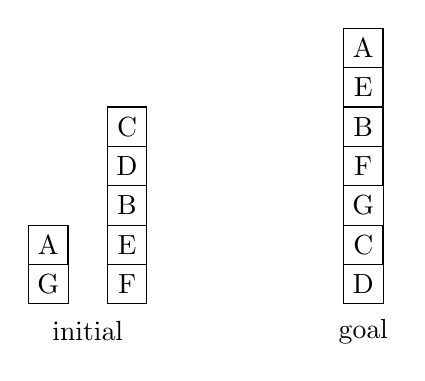
\begin{tikzpicture}
	\node[draw, minimum size=0.5cm] (G) at (0,0) {G};
	\node[draw, minimum size=0.5cm] (A) at (0,0.5) {A};

	\node[draw, minimum size=0.5cm] (F) at (1,0) {F};
	\node[draw, minimum size=0.5cm] (E) at (1,0.5) {E};
	\node[draw, minimum size=0.5cm] (B) at (1,1) {B};
	\node[draw, minimum size=0.5cm] (D) at (1,1.5) {D};
	\node[draw, minimum size=0.5cm] (C) at (1,2) {C};
	\node[] (i) at (0.5,-0.6) {initial};


	\node[draw, minimum size=0.5cm] (D) at (4,0) {D};
	\node[draw, minimum size=0.5cm] (C) at (4,0.5) {C};
	\node[draw, minimum size=0.5cm] (G) at (4,1) {G};
	\node[draw, minimum size=0.5cm] (F) at (4,1.5) {F};
	\node[draw, minimum size=0.5cm] (B) at (4,2) {B};
	\node[draw, minimum size=0.5cm] (E) at (4,2.5) {E};
	\node[draw, minimum size=0.5cm] (A) at (4,3) {A};
	\node[] (g) at (4,-0.6) {goal};
\end{tikzpicture}
\end{center}

MUGS:
\begin{itemize}
	\item $\{on(E,B), on(G,C)\}$
	\item $\{on(A,E), on(C,D), on(G,C)\}$
	\item $\{on(B,F), on(G,C)\}$
	\item $\{on(F,G)\}$
	\item $\{on(A,E), on(C,D), on(E,B)\}$
	\item $\{on(B,F), on(E,B)\}$
	\item $\{on(B,F), on(C,D)\}$
	\item $\{on(A,E), on(B,F)\}$
\end{itemize}




%% \section*{Acknowledgments}
%
%% This material is based upon work supported by the Air Force Office
%% of Scientific Research under award number FA9550-18-1-0245. J\"org
%% Hoffmann's group has also received support by the German Research
%% Foundation (DFG) as part of CRC 248 (see
%% perspicuous-computing.science). Part of this work was performed
%% while J\"org Hoffmann was visiting NASA Ames Research Center. We
%% thank J.\ Benton, Minh Do, Jeremy Frank, and David Smith for
%% insightful discussions.

\ifdefined\longflagdefined

\bibliographystyle{named}
\bibliography{abbreviations,biblio,crossref}

\else 

\bibliographystyle{named}
\bibliography{abbreviations,biblio,crossref-short}

\fi





\ifdefined\suppflagdefined

\appendix


\section{XAIP Comments}

\paragraph{verbalizing plans}

	Comment: I was thinking about the plan verbalization work from Manuela Veloso's group 
	-- e.g. \url{https://www.ijcai.org/Proceedings/16/Papers/127.pdf} 
	-- and realized there may be some interesting connections here. 
	Granted these are different kinds of plans, motion plans versus plans in general, 
	but...  I wonder if an approach like in this paper can be a better alternative 
	to the template approach in the verbalization work. For example, a PDO versus 
	a concrete PDO could help with "specificity" while planning models do have 
	a rich literature of abstractions that can be readily leveraged in this framework. 
	I guess the point is if it is useful automating the templatization using plan properties. 
	Maybe something to think about... 

	More (recent) details here if you are interested:
	\begin{enumerate}
		\item \url{http://www.cs.cmu.edu/~mmv/papers/18gcai-PereraVeloso.pdf}
		\item (data you can use) \url{http://www.cs.cmu.edu/~vdperera/paper/vdperera_thesis.pdf#page=129}
	\end{enumerate}

\section{Full Data for Action-Set Property Experiments}
\label{data-action-set-properties}

\joerg{Rebecca insert individual figures with plots for each of the 4
  domains}


%\begin{figure*}[ht]
%
\tiny
\begin{tikzpicture}


\begin{axis}[
width = 7cm,
height=4cm,
enlarge x limits = 0.1,
enlarge y limits = 0.1,
ybar,
bar width=1pt,
ymin = 0,
ymax = 10,
at={(0.0\linewidth,-0.0)},
compat=1.6,
title=c 100,
ylabel=goals 4,
]
\addplot+[ybar, bar shift =-2.5pt, red,
]
plot coordinates {
(07, 10)
(08, 10)
(01, 10)
(09, 10)
(06, 10)
(03, 10)
(04, 10)
(05, 10)
(02, 10)
(10, 9)
};
\label{plot:properties_hff_bu_55}
\addplot+[ybar, bar shift =-0.5pt, blue,
]
plot coordinates {
(08, 10)
(01, 10)
(07, 10)
(09, 9)
(06, 10)
(03, 10)
(04, 10)
(05, 10)
(02, 10)
(10, 9)
};
\label{plot:properties_hff_td_55}
\addplot+[ybar, bar shift =0.5pt, darkgreen,
]
plot coordinates {
(05, 10)
(08, 10)
(07, 10)
(09, 10)
(03, 10)
(04, 10)
(06, 10)
(01, 10)
(10, 10)
(02, 10)
};
\label{plot:properties_trap_prefop_bu_55}
\addplot+[ybar, bar shift =2.5pt, orange,
]
plot coordinates {
(07, 10)
(05, 10)
(04, 10)
(08, 10)
(09, 10)
(03, 10)
(06, 10)
(01, 10)
(10, 10)
(02, 10)
};
\label{plot:properties_trap_prefop_td_55}

\end{axis}
\hfill


\begin{axis}[
width = 7cm,
height=4cm,
enlarge x limits = 0.1,
enlarge y limits = 0.1,
ybar,
bar width=1pt,
ymin = 0,
ymax = 10,
at={(0.333333333333\linewidth,-0.0)},
compat=1.6,
title=c 150,
]
\addplot+[ybar, bar shift =-2.5pt, red,
]
plot coordinates {
(05, 9)
(04, 10)
(03, 10)
(10, 1)
(02, 10)
(06, 8)
(09, 1)
(08, 2)
(07, 5)
(01, 10)
};
\label{plot:properties_hff_bu_55}
\addplot+[ybar, bar shift =-0.5pt, blue,
]
plot coordinates {
(05, 9)
(04, 10)
(10, 0)
(02, 10)
(09, 0)
(08, 2)
(03, 10)
(07, 3)
(06, 7)
(01, 10)
};
\label{plot:properties_hff_td_55}
\addplot+[ybar, bar shift =0.5pt, darkgreen,
]
plot coordinates {
(05, 8)
(04, 9)
(10, 2)
(02, 10)
(09, 2)
(08, 3)
(03, 10)
(07, 5)
(06, 6)
(01, 10)
};
\label{plot:properties_trap_prefop_bu_55}
\addplot+[ybar, bar shift =2.5pt, orange,
]
plot coordinates {
(05, 10)
(04, 10)
(10, 2)
(02, 10)
(08, 4)
(03, 10)
(07, 6)
(06, 9)
(01, 10)
(09, 3)
};
\label{plot:properties_trap_prefop_td_55}

\end{axis}
\hfill


\begin{axis}[
width = 7cm,
height=4cm,
enlarge x limits = 0.1,
enlarge y limits = 0.1,
ybar,
bar width=1pt,
ymin = 0,
ymax = 10,
at={(0.666666666667\linewidth,-0.0)},
compat=1.6,
title=c 200,
]
\addplot+[ybar, bar shift =-2.5pt, red,
]
plot coordinates {
(08, 1)
(02, 10)
(03, 10)
(04, 10)
(07, 2)
(09, 0)
(01, 10)
(06, 6)
(10, 0)
(05, 10)
};
\label{plot:properties_hff_bu_55}
\addplot+[ybar, bar shift =-0.5pt, blue,
]
plot coordinates {
(07, 8)
(08, 6)
(02, 10)
(03, 10)
(04, 10)
(09, 5)
(10, 2)
(01, 10)
(06, 9)
(05, 10)
};
\label{plot:properties_hff_td_55}
\addplot+[ybar, bar shift =0.5pt, darkgreen,
]
plot coordinates {
(08, 2)
(07, 3)
(03, 10)
(06, 5)
(04, 10)
(09, 0)
(01, 10)
(02, 10)
(05, 9)
(10, 0)
};
\label{plot:properties_trap_prefop_bu_55}
\addplot+[ybar, bar shift =2.5pt, orange,
]
plot coordinates {
(08, 9)
(07, 8)
(06, 10)
(04, 10)
(01, 10)
(10, 5)
(03, 10)
(09, 8)
(02, 10)
(05, 10)
};
\label{plot:properties_trap_prefop_td_55}

\end{axis}
\hfill


\begin{axis}[
width = 7cm,
height=4cm,
enlarge x limits = 0.1,
enlarge y limits = 0.1,
ybar,
bar width=1pt,
ymin = 0,
ymax = 10,
at={(0.0\linewidth,-160.0)},
compat=1.6,
ylabel=goals 5,
]
\addplot+[ybar, bar shift =-2.5pt, red,
]
plot coordinates {
(01, 10)
(08, 9)
(05, 10)
(03, 10)
(02, 10)
(09, 9)
(04, 10)
(07, 9)
(06, 10)
(10, 9)
};
\label{plot:properties_hff_bu_55}
\addplot+[ybar, bar shift =-0.5pt, blue,
]
plot coordinates {
(01, 10)
(08, 6)
(03, 10)
(02, 10)
(09, 5)
(04, 10)
(07, 7)
(05, 10)
(06, 9)
(10, 2)
};
\label{plot:properties_hff_td_55}
\addplot+[ybar, bar shift =0.5pt, darkgreen,
]
plot coordinates {
(01, 10)
(08, 10)
(03, 10)
(02, 10)
(07, 10)
(05, 10)
(04, 10)
(09, 10)
(06, 10)
(10, 10)
};
\label{plot:properties_trap_prefop_bu_55}
\addplot+[ybar, bar shift =2.5pt, orange,
]
plot coordinates {
(01, 10)
(08, 10)
(03, 10)
(02, 10)
(09, 10)
(07, 10)
(04, 10)
(06, 10)
(10, 10)
(05, 10)
};
\label{plot:properties_trap_prefop_td_55}

\end{axis}
\hfill


\begin{axis}[
width = 7cm,
height=4cm,
enlarge x limits = 0.1,
enlarge y limits = 0.1,
ybar,
bar width=1pt,
ymin = 0,
ymax = 10,
at={(0.333333333333\linewidth,-160.0)},
compat=1.6,
]
\addplot+[ybar, bar shift =-2.5pt, red,
]
plot coordinates {
(05, 5)
(06, 2)
(10, 0)
(04, 9)
(01, 10)
(09, 0)
(02, 10)
(08, 1)
(07, 1)
(03, 10)
};
\label{plot:properties_hff_bu_55}
\addplot+[ybar, bar shift =-0.5pt, blue,
]
plot coordinates {
(05, 7)
(06, 4)
(10, 1)
(04, 9)
(01, 10)
(09, 1)
(02, 10)
(08, 1)
(07, 1)
(03, 10)
};
\label{plot:properties_hff_td_55}
\addplot+[ybar, bar shift =0.5pt, darkgreen,
]
plot coordinates {
(05, 6)
(06, 2)
(10, 1)
(04, 10)
(01, 10)
(09, 1)
(02, 10)
(08, 1)
(07, 1)
(03, 10)
};
\label{plot:properties_trap_prefop_bu_55}
\addplot+[ybar, bar shift =2.5pt, orange,
]
plot coordinates {
(05, 9)
(06, 6)
(10, 2)
(04, 10)
(01, 10)
(09, 2)
(02, 10)
(08, 3)
(07, 4)
(03, 10)
};
\label{plot:properties_trap_prefop_td_55}

\end{axis}
\hfill


\begin{axis}[
width = 7cm,
height=4cm,
enlarge x limits = 0.1,
enlarge y limits = 0.1,
ybar,
bar width=1pt,
ymin = 0,
ymax = 10,
at={(0.666666666667\linewidth,-160.0)},
compat=1.6,
]
\addplot+[ybar, bar shift =-2.5pt, red,
]
plot coordinates {
(03, 10)
(04, 7)
(05, 3)
(09, 0)
(01, 10)
(02, 10)
(08, 0)
(06, 1)
(10, 0)
(07, 0)
};
\label{plot:properties_hff_bu_55}
\addplot+[ybar, bar shift =-0.5pt, blue,
]
plot coordinates {
(03, 10)
(04, 8)
(05, 7)
(09, 5)
(01, 10)
(02, 10)
(08, 5)
(06, 7)
(10, 4)
(07, 6)
};
\label{plot:properties_hff_td_55}
\addplot+[ybar, bar shift =0.5pt, darkgreen,
]
plot coordinates {
(03, 9)
(04, 6)
(05, 1)
(09, 0)
(01, 10)
(02, 10)
(08, 0)
(06, 1)
(10, 0)
(07, 0)
};
\label{plot:properties_trap_prefop_bu_55}
\addplot+[ybar, bar shift =2.5pt, orange,
]
plot coordinates {
(03, 10)
(04, 10)
(05, 8)
(09, 5)
(01, 10)
(02, 10)
(08, 6)
(07, 8)
(06, 7)
(10, 4)
};
\label{plot:properties_trap_prefop_td_55}

\end{axis}
\hfill


\begin{axis}[
width = 7cm,
height=4cm,
enlarge x limits = 0.1,
enlarge y limits = 0.1,
ybar,
bar width=1pt,
ymin = 0,
ymax = 10,
at={(0.0\linewidth,-320.0)},
compat=1.6,
ylabel=goals 6,
]
\addplot+[ybar, bar shift =-2.5pt, red,
]
plot coordinates {
(08, 2)
(09, 2)
(01, 10)
(10, 2)
(06, 5)
(04, 8)
(07, 4)
(05, 5)
(02, 9)
(03, 8)
};
\label{plot:properties_hff_bu_55}
\addplot+[ybar, bar shift =-0.5pt, blue,
]
plot coordinates {
(06, 2)
(08, 2)
(09, 2)
(01, 10)
(10, 2)
(07, 2)
(04, 7)
(05, 4)
(02, 9)
(03, 8)
};
\label{plot:properties_hff_td_55}
\addplot+[ybar, bar shift =0.5pt, darkgreen,
]
plot coordinates {
(08, 8)
(09, 8)
(01, 10)
(10, 8)
(06, 9)
(04, 10)
(02, 10)
(05, 9)
(07, 8)
(03, 10)
};
\label{plot:properties_trap_prefop_bu_55}
\addplot+[ybar, bar shift =2.5pt, orange,
]
plot coordinates {
(08, 8)
(09, 8)
(01, 10)
(10, 7)
(06, 7)
(04, 8)
(07, 8)
(05, 7)
(03, 8)
(02, 10)
};
\label{plot:properties_trap_prefop_td_55}

\end{axis}
\hfill


\begin{axis}[
width = 7cm,
height=4cm,
enlarge x limits = 0.1,
enlarge y limits = 0.1,
ybar,
bar width=1pt,
ymin = 0,
ymax = 10,
at={(0.333333333333\linewidth,-320.0)},
compat=1.6,
]
\addplot+[ybar, bar shift =-2.5pt, red,
]
plot coordinates {
(06, 1)
(10, 0)
(03, 9)
(05, 3)
(07, 1)
(08, 1)
(02, 10)
(09, 0)
(01, 10)
(04, 7)
};
\label{plot:properties_hff_bu_55}
\addplot+[ybar, bar shift =-0.5pt, blue,
]
plot coordinates {
(06, 2)
(10, 0)
(03, 10)
(05, 4)
(08, 0)
(07, 0)
(02, 10)
(09, 0)
(01, 10)
(04, 7)
};
\label{plot:properties_hff_td_55}
\addplot+[ybar, bar shift =0.5pt, darkgreen,
]
plot coordinates {
(06, 2)
(10, 2)
(05, 2)
(08, 2)
(07, 2)
(02, 10)
(09, 2)
(01, 10)
(03, 7)
(04, 4)
};
\label{plot:properties_trap_prefop_bu_55}
\addplot+[ybar, bar shift =2.5pt, orange,
]
plot coordinates {
(06, 3)
(10, 3)
(03, 8)
(05, 4)
(07, 3)
(08, 3)
(02, 10)
(09, 3)
(01, 10)
(04, 6)
};
\label{plot:properties_trap_prefop_td_55}

\end{axis}
\hfill


\begin{axis}[
width = 7cm,
height=4cm,
enlarge x limits = 0.1,
enlarge y limits = 0.1,
ybar,
bar width=1pt,
ymin = 0,
ymax = 10,
at={(0.666666666667\linewidth,-320.0)},
compat=1.6,
]
\addplot+[ybar, bar shift =-2.5pt, red,
]
plot coordinates {
(02, 8)
(01, 10)
(04, 3)
(03, 4)
(06, 1)
(10, 0)
(05, 3)
(09, 0)
(08, 0)
(07, 0)
};
\label{plot:properties_hff_bu_55}
\addplot+[ybar, bar shift =-0.5pt, blue,
]
plot coordinates {
(02, 9)
(01, 10)
(04, 6)
(03, 7)
(08, 3)
(06, 4)
(10, 1)
(05, 6)
(09, 1)
(07, 4)
};
\label{plot:properties_hff_td_55}
\addplot+[ybar, bar shift =0.5pt, darkgreen,
]
plot coordinates {
(02, 10)
(01, 10)
(06, 1)
(04, 4)
(03, 5)
(08, 0)
(10, 0)
(05, 2)
(09, 0)
(07, 0)
};
\label{plot:properties_trap_prefop_bu_55}
\addplot+[ybar, bar shift =2.5pt, orange,
]
plot coordinates {
(02, 10)
(04, 7)
(03, 8)
(07, 5)
(08, 4)
(06, 7)
(10, 3)
(05, 7)
(09, 3)
(01, 10)
};
\label{plot:properties_trap_prefop_td_55}

\end{axis}
\hfill

\node[draw] (test) at (8,-8) {
\ref{plot:properties_hff_bu_55} properties-hff-bu
\ref{plot:properties_hff_td_55} properties-hff-td
\ref{plot:properties_trap_prefop_bu_55} properties-trap-prefop-bu
\ref{plot:properties_trap_prefop_td_55} properties-trap-prefop-td
};

\end{tikzpicture}
\hfill

%\caption{nomystery: reference coverage first node in top-down meta search tree;
%	optimal coverage always 10}
%\end{figure*}

%\begin{figure*}[ht]
%
\tiny
\begin{tikzpicture}


\begin{axis}[
width = 7cm,
height=4cm,
enlarge x limits = 0.1,
enlarge y limits = 0.1,
ybar,
bar width=1pt,
ymin = 0,
ymax = 10,
at={(0.0\linewidth,-0.0)},
compat=1.6,
title=c 100,
ylabel=goals 4,
]
\addplot+[ybar, bar shift =-2.5pt, red,
]
plot coordinates {
(04, 10)
(03, 10)
(02, 10)
(09, 10)
(01, 10)
(08, 10)
(07, 10)
(10, 10)
(06, 10)
(05, 10)
};
\label{plot:properties_hff_bu_4}
\addplot+[ybar, bar shift =-0.5pt, blue,
]
plot coordinates {
(04, 10)
(03, 10)
(02, 10)
(09, 10)
(01, 10)
(08, 10)
(07, 10)
(10, 10)
(06, 10)
(05, 10)
};
\label{plot:properties_hff_td_4}
\addplot+[ybar, bar shift =0.5pt, darkgreen,
]
plot coordinates {
(04, 10)
(03, 10)
(02, 10)
(09, 10)
(01, 10)
(08, 10)
(07, 10)
(10, 10)
(06, 10)
(05, 10)
};
\label{plot:properties_trap_prefop_bu_4}
\addplot+[ybar, bar shift =2.5pt, orange,
]
plot coordinates {
(04, 10)
(03, 10)
(02, 10)
(09, 10)
(01, 10)
(08, 10)
(07, 10)
(10, 10)
(06, 10)
(05, 10)
};
\label{plot:properties_trap_prefop_td_4}

\end{axis}
\hfill


\begin{axis}[
width = 7cm,
height=4cm,
enlarge x limits = 0.1,
enlarge y limits = 0.1,
ybar,
bar width=1pt,
ymin = 0,
ymax = 10,
at={(0.333333333333\linewidth,-0.0)},
compat=1.6,
title=c 150,
]
\addplot+[ybar, bar shift =-2.5pt, red,
]
plot coordinates {
(07, 10)
(08, 10)
(09, 10)
(01, 10)
(02, 10)
(03, 10)
(04, 10)
(05, 10)
(06, 10)
(10, 10)
};
\label{plot:properties_hff_bu_4}
\addplot+[ybar, bar shift =-0.5pt, blue,
]
plot coordinates {
(07, 10)
(08, 10)
(09, 8)
(01, 10)
(04, 10)
(02, 10)
(03, 10)
(05, 10)
(10, 4)
(06, 10)
};
\label{plot:properties_hff_td_4}
\addplot+[ybar, bar shift =0.5pt, darkgreen,
]
plot coordinates {
(07, 10)
(08, 9)
(09, 9)
(01, 10)
(02, 10)
(03, 10)
(04, 10)
(05, 10)
(06, 10)
(10, 9)
};
\label{plot:properties_trap_prefop_bu_4}
\addplot+[ybar, bar shift =2.5pt, orange,
]
plot coordinates {
(07, 10)
(08, 10)
(09, 10)
(01, 10)
(02, 10)
(03, 10)
(04, 10)
(05, 10)
(06, 10)
(10, 10)
};
\label{plot:properties_trap_prefop_td_4}

\end{axis}
\hfill


\begin{axis}[
width = 7cm,
height=4cm,
enlarge x limits = 0.1,
enlarge y limits = 0.1,
ybar,
bar width=1pt,
ymin = 0,
ymax = 10,
at={(0.666666666667\linewidth,-0.0)},
compat=1.6,
title=c 200,
]
\addplot+[ybar, bar shift =-2.5pt, red,
]
plot coordinates {
(07, 10)
(04, 10)
(05, 10)
(06, 10)
(10, 9)
(03, 10)
(08, 10)
(01, 10)
(09, 10)
(02, 10)
};
\label{plot:properties_hff_bu_4}
\addplot+[ybar, bar shift =-0.5pt, blue,
]
plot coordinates {
(05, 10)
(04, 10)
(06, 10)
(10, 8)
(07, 10)
(03, 10)
(08, 10)
(01, 10)
(09, 8)
(02, 10)
};
\label{plot:properties_hff_td_4}
\addplot+[ybar, bar shift =0.5pt, darkgreen,
]
plot coordinates {
(08, 10)
(03, 10)
(05, 10)
(04, 10)
(10, 8)
(02, 10)
(07, 10)
(01, 10)
(09, 9)
(06, 10)
};
\label{plot:properties_trap_prefop_bu_4}
\addplot+[ybar, bar shift =2.5pt, orange,
]
plot coordinates {
(05, 10)
(04, 10)
(10, 10)
(07, 10)
(03, 10)
(08, 10)
(01, 10)
(09, 10)
(06, 10)
(02, 10)
};
\label{plot:properties_trap_prefop_td_4}

\end{axis}
\hfill


\begin{axis}[
width = 7cm,
height=4cm,
enlarge x limits = 0.1,
enlarge y limits = 0.1,
ybar,
bar width=1pt,
ymin = 0,
ymax = 10,
at={(0.0\linewidth,-160.0)},
compat=1.6,
ylabel=goals 5,
]
\addplot+[ybar, bar shift =-2.5pt, red,
]
plot coordinates {
(08, 10)
(04, 10)
(09, 10)
(01, 10)
(06, 10)
(07, 10)
(02, 10)
(03, 10)
(05, 10)
(10, 10)
};
\label{plot:properties_hff_bu_4}
\addplot+[ybar, bar shift =-0.5pt, blue,
]
plot coordinates {
(03, 10)
(08, 9)
(01, 10)
(09, 7)
(07, 10)
(02, 10)
(04, 10)
(06, 10)
(05, 10)
(10, 4)
};
\label{plot:properties_hff_td_4}
\addplot+[ybar, bar shift =0.5pt, darkgreen,
]
plot coordinates {
(03, 10)
(08, 10)
(01, 10)
(09, 10)
(07, 10)
(04, 10)
(06, 10)
(05, 10)
(10, 10)
(02, 10)
};
\label{plot:properties_trap_prefop_bu_4}
\addplot+[ybar, bar shift =2.5pt, orange,
]
plot coordinates {
(08, 10)
(03, 10)
(09, 10)
(01, 10)
(06, 10)
(07, 10)
(04, 10)
(05, 10)
(10, 10)
(02, 10)
};
\label{plot:properties_trap_prefop_td_4}

\end{axis}
\hfill


\begin{axis}[
width = 7cm,
height=4cm,
enlarge x limits = 0.1,
enlarge y limits = 0.1,
ybar,
bar width=1pt,
ymin = 0,
ymax = 10,
at={(0.333333333333\linewidth,-160.0)},
compat=1.6,
]
\addplot+[ybar, bar shift =-2.5pt, red,
]
plot coordinates {
(02, 10)
(05, 10)
(10, 3)
(04, 10)
(07, 7)
(06, 9)
(09, 3)
(01, 10)
(08, 6)
(03, 10)
};
\label{plot:properties_hff_bu_4}
\addplot+[ybar, bar shift =-0.5pt, blue,
]
plot coordinates {
(02, 10)
(10, 2)
(05, 10)
(04, 10)
(07, 7)
(06, 9)
(09, 2)
(01, 10)
(08, 5)
(03, 10)
};
\label{plot:properties_hff_td_4}
\addplot+[ybar, bar shift =0.5pt, darkgreen,
]
plot coordinates {
(02, 10)
(10, 5)
(05, 10)
(04, 10)
(07, 9)
(06, 10)
(09, 8)
(01, 10)
(08, 8)
(03, 10)
};
\label{plot:properties_trap_prefop_bu_4}
\addplot+[ybar, bar shift =2.5pt, orange,
]
plot coordinates {
(02, 10)
(10, 7)
(04, 10)
(05, 10)
(07, 10)
(06, 10)
(09, 10)
(01, 10)
(08, 10)
(03, 10)
};
\label{plot:properties_trap_prefop_td_4}

\end{axis}
\hfill


\begin{axis}[
width = 7cm,
height=4cm,
enlarge x limits = 0.1,
enlarge y limits = 0.1,
ybar,
bar width=1pt,
ymin = 0,
ymax = 10,
at={(0.666666666667\linewidth,-160.0)},
compat=1.6,
]
\addplot+[ybar, bar shift =-2.5pt, red,
]
plot coordinates {
(02, 10)
(05, 10)
(04, 10)
(07, 9)
(06, 10)
(10, 8)
(03, 10)
(09, 9)
(01, 10)
(08, 9)
};
\label{plot:properties_hff_bu_4}
\addplot+[ybar, bar shift =-0.5pt, blue,
]
plot coordinates {
(03, 10)
(02, 10)
(10, 8)
(05, 10)
(04, 10)
(07, 9)
(06, 10)
(09, 9)
(01, 10)
(08, 9)
};
\label{plot:properties_hff_td_4}
\addplot+[ybar, bar shift =0.5pt, darkgreen,
]
plot coordinates {
(07, 9)
(03, 10)
(02, 10)
(10, 6)
(05, 10)
(04, 10)
(06, 10)
(09, 7)
(01, 10)
(08, 8)
};
\label{plot:properties_trap_prefop_bu_4}
\addplot+[ybar, bar shift =2.5pt, orange,
]
plot coordinates {
(03, 10)
(02, 10)
(10, 9)
(05, 10)
(04, 10)
(07, 10)
(06, 10)
(09, 10)
(01, 10)
(08, 10)
};
\label{plot:properties_trap_prefop_td_4}

\end{axis}
\hfill


\begin{axis}[
width = 7cm,
height=4cm,
enlarge x limits = 0.1,
enlarge y limits = 0.1,
ybar,
bar width=1pt,
ymin = 0,
ymax = 10,
at={(0.0\linewidth,-320.0)},
compat=1.6,
ylabel=goals 6,
]
\addplot+[ybar, bar shift =-2.5pt, red,
]
plot coordinates {
(10, 7)
(09, 8)
(02, 10)
(05, 10)
(03, 10)
(06, 10)
(01, 10)
(08, 9)
(07, 9)
(04, 10)
};
\label{plot:properties_hff_bu_4}
\addplot+[ybar, bar shift =-0.5pt, blue,
]
plot coordinates {
(09, 0)
(02, 10)
(07, 4)
(05, 9)
(03, 10)
(04, 10)
(10, 0)
(01, 10)
(08, 1)
(06, 8)
};
\label{plot:properties_hff_td_4}
\addplot+[ybar, bar shift =0.5pt, darkgreen,
]
plot coordinates {
(10, 10)
(04, 10)
(05, 10)
(07, 10)
(06, 10)
(01, 10)
(02, 10)
(09, 10)
(08, 10)
(03, 10)
};
\label{plot:properties_trap_prefop_bu_4}
\addplot+[ybar, bar shift =2.5pt, orange,
]
plot coordinates {
(10, 10)
(09, 10)
(02, 10)
(05, 10)
(04, 10)
(03, 10)
(07, 10)
(01, 10)
(08, 10)
(06, 10)
};
\label{plot:properties_trap_prefop_td_4}

\end{axis}
\hfill


\begin{axis}[
width = 7cm,
height=4cm,
enlarge x limits = 0.1,
enlarge y limits = 0.1,
ybar,
bar width=1pt,
ymin = 0,
ymax = 10,
at={(0.333333333333\linewidth,-320.0)},
compat=1.6,
]
\addplot+[ybar, bar shift =-2.5pt, red,
]
plot coordinates {
(10, 2)
(02, 10)
(03, 10)
(08, 3)
(01, 10)
(06, 5)
(07, 3)
(09, 2)
(04, 9)
(05, 8)
};
\label{plot:properties_hff_bu_4}
\addplot+[ybar, bar shift =-0.5pt, blue,
]
plot coordinates {
(10, 3)
(02, 10)
(03, 10)
(08, 3)
(01, 10)
(06, 5)
(07, 3)
(09, 3)
(04, 9)
(05, 8)
};
\label{plot:properties_hff_td_4}
\addplot+[ybar, bar shift =0.5pt, darkgreen,
]
plot coordinates {
(10, 4)
(02, 10)
(03, 10)
(08, 6)
(01, 10)
(09, 5)
(06, 10)
(07, 7)
(04, 10)
(05, 10)
};
\label{plot:properties_trap_prefop_bu_4}
\addplot+[ybar, bar shift =2.5pt, orange,
]
plot coordinates {
(10, 5)
(02, 10)
(03, 10)
(08, 8)
(01, 10)
(06, 10)
(07, 9)
(09, 6)
(04, 10)
(05, 10)
};
\label{plot:properties_trap_prefop_td_4}

\end{axis}
\hfill


\begin{axis}[
width = 7cm,
height=4cm,
enlarge x limits = 0.1,
enlarge y limits = 0.1,
ybar,
bar width=1pt,
ymin = 0,
ymax = 10,
at={(0.666666666667\linewidth,-320.0)},
compat=1.6,
]
\addplot+[ybar, bar shift =-2.5pt, red,
]
plot coordinates {
(04, 10)
(05, 10)
(02, 10)
(03, 10)
(06, 9)
(08, 8)
(09, 8)
(01, 10)
(07, 8)
(10, 7)
};
\label{plot:properties_hff_bu_4}
\addplot+[ybar, bar shift =-0.5pt, blue,
]
plot coordinates {
(04, 10)
(05, 10)
(02, 10)
(03, 10)
(06, 9)
(08, 8)
(09, 8)
(01, 10)
(07, 9)
(10, 7)
};
\label{plot:properties_hff_td_4}
\addplot+[ybar, bar shift =0.5pt, darkgreen,
]
plot coordinates {
(04, 10)
(05, 10)
(02, 10)
(03, 10)
(08, 6)
(09, 4)
(01, 10)
(06, 10)
(07, 7)
(10, 3)
};
\label{plot:properties_trap_prefop_bu_4}
\addplot+[ybar, bar shift =2.5pt, orange,
]
plot coordinates {
(04, 10)
(05, 10)
(02, 10)
(03, 10)
(08, 10)
(09, 9)
(01, 10)
(06, 10)
(07, 10)
(10, 8)
};
\label{plot:properties_trap_prefop_td_4}

\end{axis}
\hfill

\node[draw] (test) at (8,-8) {
\ref{plot:properties_hff_bu_4} properties-hff-bu
\ref{plot:properties_hff_td_4} properties-hff-td
\ref{plot:properties_trap_prefop_bu_4} properties-trap-prefop-bu
\ref{plot:properties_trap_prefop_td_4} properties-trap-prefop-td
};

\end{tikzpicture}
\hfill

%\caption{TPP: reference coverage first node in top-down meta search tree;
%	optimal coverage always 10}
%\end{figure*}

%\begin{figure*}[ht]
%
\tiny
\begin{tikzpicture}


\begin{axis}[
width = 7cm,
height=4cm,
enlarge x limits = 0.1,
enlarge y limits = 0.1,
ybar,
bar width=1pt,
ymin = 0,
ymax = 10,
at={(0.0\linewidth,-0.0)},
compat=1.6,
title=c 100,
ylabel=goals 05,
]
\addplot+[ybar, bar shift =-2.5pt, red,
]
plot coordinates {
(05, 10)
(04, 10)
(06, 9)
(02, 10)
(10, 6)
(01, 10)
(08, 9)
(09, 7)
(03, 10)
(07, 8)
};
\label{plot:properties_hff_bu_52}
\addplot+[ybar, bar shift =-1.0pt, blue,
]
plot coordinates {
(06, 9)
(10, 4)
(05, 10)
(04, 10)
(02, 10)
(01, 10)
(08, 5)
(09, 5)
(07, 7)
(03, 10)
};
\label{plot:properties_hff_td_52}
\addplot+[ybar, bar shift =1.0pt, darkgreen,
]
plot coordinates {
(06, 10)
(10, 10)
(05, 10)
(04, 10)
(03, 10)
(02, 10)
(01, 10)
(08, 10)
(09, 10)
(07, 10)
};
\label{plot:properties_trap_prefop_bu_52}
\addplot+[ybar, bar shift =2.5pt, orange,
]
plot coordinates {
(06, 10)
(05, 10)
(03, 10)
(07, 10)
(10, 10)
(02, 10)
(01, 10)
(08, 10)
(09, 10)
(04, 10)
};
\label{plot:properties_trap_prefop_td_52}
\addplot+[only marks, mark = -, mark options = {thick, red, dashed}, mark size = 0.2cm, black,
]
plot coordinates {
(08, 6)
(06, 6)
(05, 8)
(03, 9)
(01, 10)
(09, 6)
(07, 4)
(10, 4)
(04, 8)
(02, 10)
};

\end{axis}
\hfill


\begin{axis}[
width = 7cm,
height=4cm,
enlarge x limits = 0.1,
enlarge y limits = 0.1,
ybar,
bar width=1pt,
ymin = 0,
ymax = 10,
at={(0.333333333333\linewidth,-0.0)},
compat=1.6,
title=c 150,
]
\addplot+[ybar, bar shift =-2.5pt, red,
]
plot coordinates {
(08, 5)
(01, 10)
(09, 5)
(06, 8)
(07, 5)
(04, 9)
(05, 10)
(10, 4)
(02, 10)
(03, 9)
};
\label{plot:properties_hff_bu_52}
\addplot+[ybar, bar shift =-1.0pt, blue,
]
plot coordinates {
(01, 10)
(08, 4)
(09, 4)
(06, 4)
(07, 4)
(04, 9)
(05, 9)
(10, 4)
(02, 10)
(03, 9)
};
\label{plot:properties_hff_td_52}
\addplot+[ybar, bar shift =1.0pt, darkgreen,
]
plot coordinates {
(08, 10)
(01, 10)
(09, 10)
(06, 10)
(07, 10)
(04, 10)
(05, 10)
(10, 10)
(02, 10)
(03, 10)
};
\label{plot:properties_trap_prefop_bu_52}
\addplot+[ybar, bar shift =2.5pt, orange,
]
plot coordinates {
(08, 10)
(01, 10)
(09, 10)
(06, 10)
(07, 10)
(04, 10)
(05, 10)
(10, 10)
(02, 10)
(03, 10)
};
\label{plot:properties_trap_prefop_td_52}
\addplot+[only marks, mark = -, mark options = {thick, red, dashed}, mark size = 0.2cm, black,
]
plot coordinates {
(08, 6)
(06, 6)
(05, 8)
(03, 9)
(01, 10)
(09, 6)
(07, 4)
(10, 4)
(04, 8)
(02, 10)
};

\end{axis}
\hfill


\begin{axis}[
width = 7cm,
height=4cm,
enlarge x limits = 0.1,
enlarge y limits = 0.1,
ybar,
bar width=1pt,
ymin = 0,
ymax = 10,
at={(0.666666666667\linewidth,-0.0)},
compat=1.6,
title=c 200,
]
\addplot+[ybar, bar shift =-2.5pt, red,
]
plot coordinates {
(08, 8)
(04, 10)
(05, 10)
(10, 6)
(02, 10)
(03, 10)
(09, 9)
(01, 10)
(06, 7)
(07, 6)
};
\label{plot:properties_hff_bu_52}
\addplot+[ybar, bar shift =-1.0pt, blue,
]
plot coordinates {
(04, 10)
(05, 10)
(10, 7)
(02, 10)
(03, 10)
(08, 8)
(09, 9)
(01, 10)
(06, 7)
(07, 6)
};
\label{plot:properties_hff_td_52}
\addplot+[ybar, bar shift =1.0pt, darkgreen,
]
plot coordinates {
(04, 10)
(05, 10)
(10, 10)
(02, 10)
(03, 10)
(08, 10)
(09, 10)
(01, 10)
(06, 10)
(07, 10)
};
\label{plot:properties_trap_prefop_bu_52}
\addplot+[ybar, bar shift =2.5pt, orange,
]
plot coordinates {
(04, 10)
(05, 10)
(10, 10)
(02, 10)
(03, 10)
(08, 10)
(09, 10)
(01, 10)
(06, 10)
(07, 10)
};
\label{plot:properties_trap_prefop_td_52}
\addplot+[only marks, mark = -, mark options = {thick, red, dashed}, mark size = 0.2cm, black,
]
plot coordinates {
(08, 6)
(06, 6)
(05, 8)
(03, 9)
(01, 10)
(09, 6)
(07, 4)
(10, 4)
(04, 8)
(02, 10)
};

\end{axis}
\hfill


\begin{axis}[
width = 7cm,
height=4cm,
enlarge x limits = 0.1,
enlarge y limits = 0.1,
ybar,
bar width=1pt,
ymin = 0,
ymax = 10,
at={(0.0\linewidth,-160.0)},
compat=1.6,
ylabel=goals 06,
]
\addplot+[ybar, bar shift =-2.5pt, red,
]
plot coordinates {
(02, 10)
(03, 10)
(04, 10)
(05, 9)
(10, 7)
(06, 8)
(07, 7)
(08, 8)
(01, 10)
(09, 5)
};
\label{plot:properties_hff_bu_52}
\addplot+[ybar, bar shift =-1.0pt, blue,
]
plot coordinates {
(02, 10)
(03, 10)
(04, 10)
(05, 8)
(10, 4)
(06, 8)
(07, 7)
(08, 8)
(01, 10)
(09, 5)
};
\label{plot:properties_hff_td_52}
\addplot+[ybar, bar shift =1.0pt, darkgreen,
]
plot coordinates {
(02, 10)
(03, 10)
(04, 10)
(05, 10)
(10, 10)
(06, 10)
(07, 10)
(08, 10)
(01, 10)
(09, 10)
};
\label{plot:properties_trap_prefop_bu_52}
\addplot+[ybar, bar shift =2.5pt, orange,
]
plot coordinates {
(02, 10)
(03, 10)
(10, 10)
(04, 10)
(05, 10)
(06, 10)
(07, 10)
(08, 10)
(01, 10)
(09, 10)
};
\label{plot:properties_trap_prefop_td_52}
\addplot+[only marks, mark = -, mark options = {thick, red, dashed}, mark size = 0.2cm, black,
]
plot coordinates {
(04, 7)
(06, 7)
(10, 1)
(02, 9)
(08, 3)
(09, 2)
(05, 5)
(07, 3)
(01, 10)
(03, 8)
};

\end{axis}
\hfill


\begin{axis}[
width = 7cm,
height=4cm,
enlarge x limits = 0.1,
enlarge y limits = 0.1,
ybar,
bar width=1pt,
ymin = 0,
ymax = 10,
at={(0.333333333333\linewidth,-160.0)},
compat=1.6,
]
\addplot+[ybar, bar shift =-2.5pt, red,
]
plot coordinates {
(07, 8)
(06, 7)
(01, 10)
(09, 5)
(08, 5)
(03, 10)
(10, 4)
(02, 10)
(05, 9)
(04, 10)
};
\label{plot:properties_hff_bu_52}
\addplot+[ybar, bar shift =-1.0pt, blue,
]
plot coordinates {
(07, 6)
(06, 6)
(01, 10)
(09, 5)
(08, 5)
(03, 10)
(10, 4)
(02, 10)
(05, 9)
(04, 10)
};
\label{plot:properties_hff_td_52}
\addplot+[ybar, bar shift =1.0pt, darkgreen,
]
plot coordinates {
(07, 10)
(06, 10)
(01, 10)
(09, 10)
(08, 10)
(03, 10)
(10, 10)
(02, 10)
(05, 10)
(04, 10)
};
\label{plot:properties_trap_prefop_bu_52}
\addplot+[ybar, bar shift =2.5pt, orange,
]
plot coordinates {
(07, 10)
(06, 10)
(01, 10)
(09, 10)
(08, 10)
(03, 10)
(10, 10)
(02, 10)
(05, 10)
(04, 10)
};
\label{plot:properties_trap_prefop_td_52}
\addplot+[only marks, mark = -, mark options = {thick, red, dashed}, mark size = 0.2cm, black,
]
plot coordinates {
(04, 7)
(06, 7)
(10, 1)
(02, 9)
(08, 3)
(09, 2)
(05, 5)
(07, 3)
(01, 10)
(03, 8)
};

\end{axis}
\hfill


\begin{axis}[
width = 7cm,
height=4cm,
enlarge x limits = 0.1,
enlarge y limits = 0.1,
ybar,
bar width=1pt,
ymin = 0,
ymax = 10,
at={(0.666666666667\linewidth,-160.0)},
compat=1.6,
]
\addplot+[ybar, bar shift =-2.5pt, red,
]
plot coordinates {
(08, 4)
(09, 5)
(01, 10)
(07, 7)
(03, 10)
(10, 4)
(04, 10)
(02, 10)
(05, 9)
(06, 5)
};
\label{plot:properties_hff_bu_52}
\addplot+[ybar, bar shift =-1.0pt, blue,
]
plot coordinates {
(09, 8)
(08, 7)
(07, 8)
(01, 10)
(10, 4)
(02, 10)
(05, 9)
(03, 10)
(04, 10)
(06, 5)
};
\label{plot:properties_hff_td_52}
\addplot+[ybar, bar shift =1.0pt, darkgreen,
]
plot coordinates {
(08, 10)
(01, 10)
(09, 10)
(03, 10)
(06, 10)
(10, 10)
(04, 10)
(02, 10)
(05, 10)
(07, 10)
};
\label{plot:properties_trap_prefop_bu_52}
\addplot+[ybar, bar shift =2.5pt, orange,
]
plot coordinates {
(09, 10)
(01, 10)
(08, 10)
(07, 10)
(10, 10)
(04, 10)
(02, 10)
(05, 10)
(03, 10)
(06, 10)
};
\label{plot:properties_trap_prefop_td_52}
\addplot+[only marks, mark = -, mark options = {thick, red, dashed}, mark size = 0.2cm, black,
]
plot coordinates {
(04, 7)
(06, 7)
(10, 1)
(02, 9)
(08, 3)
(09, 2)
(05, 5)
(07, 3)
(01, 10)
(03, 8)
};

\end{axis}
\hfill


\begin{axis}[
width = 7cm,
height=4cm,
enlarge x limits = 0.1,
enlarge y limits = 0.1,
ybar,
bar width=1pt,
ymin = 0,
ymax = 10,
at={(0.0\linewidth,-320.0)},
compat=1.6,
ylabel=goals 07,
]
\addplot+[ybar, bar shift =-2.5pt, red,
]
plot coordinates {
(05, 7)
(04, 8)
(07, 3)
(06, 4)
(09, 4)
(01, 10)
(08, 4)
(03, 9)
(02, 10)
(10, 2)
};
\label{plot:properties_hff_bu_52}
\addplot+[ybar, bar shift =-1.0pt, blue,
]
plot coordinates {
(04, 8)
(07, 2)
(06, 3)
(09, 2)
(01, 10)
(08, 4)
(05, 7)
(03, 9)
(02, 10)
(10, 2)
};
\label{plot:properties_hff_td_52}
\addplot+[ybar, bar shift =1.0pt, darkgreen,
]
plot coordinates {
(04, 10)
(07, 10)
(06, 10)
(09, 10)
(01, 10)
(08, 10)
(05, 10)
(03, 10)
(02, 10)
(10, 10)
};
\label{plot:properties_trap_prefop_bu_52}
\addplot+[ybar, bar shift =2.5pt, orange,
]
plot coordinates {
(05, 10)
(04, 10)
(07, 10)
(06, 10)
(09, 10)
(01, 10)
(08, 10)
(03, 10)
(02, 10)
(10, 10)
};
\label{plot:properties_trap_prefop_td_52}
\addplot+[only marks, mark = -, mark options = {thick, red, dashed}, mark size = 0.2cm, black,
]
plot coordinates {
(03, 7)
(05, 6)
(07, 0)
(09, 3)
(01, 9)
(02, 8)
(04, 7)
(06, 2)
(08, 3)
(10, 2)
};

\end{axis}
\hfill


\begin{axis}[
width = 7cm,
height=4cm,
enlarge x limits = 0.1,
enlarge y limits = 0.1,
ybar,
bar width=1pt,
ymin = 0,
ymax = 10,
at={(0.333333333333\linewidth,-320.0)},
compat=1.6,
]
\addplot+[ybar, bar shift =-2.5pt, red,
]
plot coordinates {
(08, 4)
(09, 3)
(01, 10)
(03, 8)
(02, 10)
(04, 9)
(05, 10)
(06, 6)
(10, 2)
(07, 6)
};
\label{plot:properties_hff_bu_52}
\addplot+[ybar, bar shift =-1.0pt, blue,
]
plot coordinates {
(01, 10)
(08, 5)
(02, 10)
(04, 9)
(03, 8)
(05, 10)
(06, 5)
(10, 5)
(07, 7)
(09, 6)
};
\label{plot:properties_hff_td_52}
\addplot+[ybar, bar shift =1.0pt, darkgreen,
]
plot coordinates {
(09, 10)
(01, 10)
(02, 10)
(04, 10)
(03, 10)
(05, 10)
(06, 10)
(10, 10)
(07, 10)
(08, 10)
};
\label{plot:properties_trap_prefop_bu_52}
\addplot+[ybar, bar shift =2.5pt, orange,
]
plot coordinates {
(01, 10)
(08, 10)
(02, 10)
(03, 10)
(04, 10)
(05, 10)
(06, 10)
(10, 10)
(07, 10)
(09, 10)
};
\label{plot:properties_trap_prefop_td_52}
\addplot+[only marks, mark = -, mark options = {thick, red, dashed}, mark size = 0.2cm, black,
]
plot coordinates {
(03, 7)
(05, 6)
(07, 0)
(09, 3)
(01, 9)
(02, 8)
(04, 7)
(06, 2)
(08, 3)
(10, 2)
};

\end{axis}
\hfill


\begin{axis}[
width = 7cm,
height=4cm,
enlarge x limits = 0.1,
enlarge y limits = 0.1,
ybar,
bar width=1pt,
ymin = 0,
ymax = 10,
at={(0.666666666667\linewidth,-320.0)},
compat=1.6,
]
\addplot+[ybar, bar shift =-2.5pt, red,
]
plot coordinates {
(08, 4)
(07, 8)
(01, 10)
(09, 5)
(02, 10)
(03, 10)
(04, 10)
(05, 10)
(06, 8)
(10, 2)
};
\label{plot:properties_hff_bu_52}
\addplot+[ybar, bar shift =-1.0pt, blue,
]
plot coordinates {
(08, 5)
(07, 9)
(01, 10)
(09, 7)
(03, 10)
(05, 10)
(04, 10)
(06, 8)
(02, 10)
(10, 7)
};
\label{plot:properties_hff_td_52}
\addplot+[ybar, bar shift =1.0pt, darkgreen,
]
plot coordinates {
(08, 10)
(09, 10)
(03, 10)
(05, 10)
(04, 10)
(06, 10)
(02, 10)
(10, 10)
(07, 10)
(01, 10)
};
\label{plot:properties_trap_prefop_bu_52}
\addplot+[ybar, bar shift =2.5pt, orange,
]
plot coordinates {
(08, 10)
(07, 10)
(09, 10)
(03, 10)
(04, 10)
(05, 10)
(06, 10)
(02, 10)
(10, 10)
(01, 10)
};
\label{plot:properties_trap_prefop_td_52}
\addplot+[only marks, mark = -, mark options = {thick, red, dashed}, mark size = 0.2cm, black,
]
plot coordinates {
(03, 7)
(05, 6)
(07, 0)
(09, 3)
(01, 9)
(02, 8)
(04, 7)
(06, 2)
(08, 3)
(10, 2)
};

\end{axis}
\hfill


\begin{axis}[
width = 7cm,
height=4cm,
enlarge x limits = 0.1,
enlarge y limits = 0.1,
ybar,
bar width=1pt,
ymin = 0,
ymax = 10,
at={(0.0\linewidth,-480.0)},
compat=1.6,
ylabel=goals 08,
]
\addplot+[ybar, bar shift =-2.5pt, red,
]
plot coordinates {
(04, 6)
(05, 6)
(02, 10)
(10, 3)
(03, 9)
(08, 3)
(09, 4)
(06, 6)
(07, 4)
(01, 9)
};
\label{plot:properties_hff_bu_52}
\addplot+[ybar, bar shift =-1.0pt, blue,
]
plot coordinates {
(04, 6)
(05, 6)
(02, 10)
(10, 3)
(03, 9)
(08, 3)
(09, 4)
(06, 5)
(07, 5)
(01, 9)
};
\label{plot:properties_hff_td_52}
\addplot+[ybar, bar shift =1.0pt, darkgreen,
]
plot coordinates {
(01, 10)
(04, 10)
(05, 10)
(02, 10)
(10, 10)
(03, 10)
(08, 10)
(09, 10)
(06, 10)
(07, 10)
};
\label{plot:properties_trap_prefop_bu_52}
\addplot+[ybar, bar shift =2.5pt, orange,
]
plot coordinates {
(04, 10)
(05, 10)
(02, 10)
(10, 10)
(03, 10)
(08, 10)
(09, 10)
(01, 10)
(06, 10)
(07, 10)
};
\label{plot:properties_trap_prefop_td_52}
\addplot+[only marks, mark = -, mark options = {thick, red, dashed}, mark size = 0.2cm, black,
]
plot coordinates {
(08, 0)
(06, 3)
(03, 7)
(01, 8)
(05, 3)
(09, 1)
(10, 0)
(07, 2)
(02, 7)
(04, 6)
};

\end{axis}
\hfill


\begin{axis}[
width = 7cm,
height=4cm,
enlarge x limits = 0.1,
enlarge y limits = 0.1,
ybar,
bar width=1pt,
ymin = 0,
ymax = 10,
at={(0.333333333333\linewidth,-480.0)},
compat=1.6,
]
\addplot+[ybar, bar shift =-2.5pt, red,
]
plot coordinates {
(02, 10)
(09, 4)
(01, 10)
(08, 3)
(07, 4)
(06, 6)
(10, 2)
(05, 8)
(04, 8)
(03, 10)
};
\label{plot:properties_hff_bu_52}
\addplot+[ybar, bar shift =-1.0pt, blue,
]
plot coordinates {
(02, 10)
(09, 4)
(01, 10)
(08, 3)
(07, 5)
(06, 7)
(10, 2)
(05, 8)
(04, 8)
(03, 10)
};
\label{plot:properties_hff_td_52}
\addplot+[ybar, bar shift =1.0pt, darkgreen,
]
plot coordinates {
(02, 10)
(09, 10)
(01, 10)
(08, 10)
(07, 10)
(06, 10)
(10, 10)
(05, 10)
(04, 10)
(03, 10)
};
\label{plot:properties_trap_prefop_bu_52}
\addplot+[ybar, bar shift =2.5pt, orange,
]
plot coordinates {
(02, 10)
(09, 10)
(01, 10)
(08, 10)
(07, 10)
(06, 10)
(10, 10)
(05, 10)
(04, 10)
(03, 10)
};
\label{plot:properties_trap_prefop_td_52}
\addplot+[only marks, mark = -, mark options = {thick, red, dashed}, mark size = 0.2cm, black,
]
plot coordinates {
(08, 0)
(06, 3)
(03, 7)
(01, 8)
(05, 3)
(09, 1)
(10, 0)
(07, 2)
(02, 7)
(04, 6)
};

\end{axis}
\hfill


\begin{axis}[
width = 7cm,
height=4cm,
enlarge x limits = 0.1,
enlarge y limits = 0.1,
ybar,
bar width=1pt,
ymin = 0,
ymax = 10,
at={(0.666666666667\linewidth,-480.0)},
compat=1.6,
]
\addplot+[ybar, bar shift =-2.5pt, red,
]
plot coordinates {
(09, 4)
(03, 9)
(04, 9)
(07, 8)
(08, 5)
(10, 3)
(06, 7)
(01, 10)
(05, 7)
(02, 10)
};
\label{plot:properties_hff_bu_52}
\addplot+[ybar, bar shift =-1.0pt, blue,
]
plot coordinates {
(02, 10)
(03, 10)
(01, 10)
(04, 9)
(08, 7)
(06, 9)
(07, 8)
(10, 4)
(09, 5)
(05, 8)
};
\label{plot:properties_hff_td_52}
\addplot+[ybar, bar shift =1.0pt, darkgreen,
]
plot coordinates {
(03, 10)
(05, 10)
(08, 10)
(07, 10)
(10, 10)
(06, 10)
(09, 10)
(01, 10)
(02, 10)
(04, 10)
};
\label{plot:properties_trap_prefop_bu_52}
\addplot+[ybar, bar shift =2.5pt, orange,
]
plot coordinates {
(02, 10)
(01, 10)
(03, 10)
(04, 10)
(07, 10)
(08, 10)
(10, 10)
(06, 10)
(09, 10)
(05, 10)
};
\label{plot:properties_trap_prefop_td_52}
\addplot+[only marks, mark = -, mark options = {thick, red, dashed}, mark size = 0.2cm, black,
]
plot coordinates {
(08, 0)
(06, 3)
(03, 7)
(01, 8)
(05, 3)
(09, 1)
(10, 0)
(07, 2)
(02, 7)
(04, 6)
};

\end{axis}
\hfill


\begin{axis}[
width = 7cm,
height=4cm,
enlarge x limits = 0.1,
enlarge y limits = 0.1,
ybar,
bar width=1pt,
ymin = 0,
ymax = 10,
at={(0.0\linewidth,-640.0)},
compat=1.6,
ylabel=goals 09,
]
\addplot+[ybar, bar shift =-2.5pt, red,
]
plot coordinates {
(02, 10)
(01, 10)
(09, 4)
(08, 4)
(07, 4)
(06, 6)
(10, 4)
(05, 6)
(04, 7)
(03, 8)
};
\label{plot:properties_hff_bu_52}
\addplot+[ybar, bar shift =-1.0pt, blue,
]
plot coordinates {
(02, 10)
(01, 10)
(09, 4)
(05, 6)
(08, 5)
(07, 4)
(06, 4)
(10, 4)
(04, 7)
(03, 8)
};
\label{plot:properties_hff_td_52}
\addplot+[ybar, bar shift =1.0pt, darkgreen,
]
plot coordinates {
(02, 10)
(01, 10)
(09, 10)
(05, 10)
(08, 10)
(07, 10)
(06, 10)
(10, 10)
(04, 10)
(03, 10)
};
\label{plot:properties_trap_prefop_bu_52}
\addplot+[ybar, bar shift =2.5pt, orange,
]
plot coordinates {
(02, 10)
(01, 10)
(09, 10)
(05, 10)
(08, 10)
(07, 10)
(06, 10)
(10, 10)
(04, 10)
(03, 10)
};
\label{plot:properties_trap_prefop_td_52}
\addplot+[only marks, mark = -, mark options = {thick, red, dashed}, mark size = 0.2cm, black,
]
plot coordinates {
(03, 5)
(05, 4)
(01, 7)
(07, 0)
(08, 1)
(10, 0)
(06, 0)
(09, 0)
(02, 3)
(04, 1)
};

\end{axis}
\hfill


\begin{axis}[
width = 7cm,
height=4cm,
enlarge x limits = 0.1,
enlarge y limits = 0.1,
ybar,
bar width=1pt,
ymin = 0,
ymax = 10,
at={(0.333333333333\linewidth,-640.0)},
compat=1.6,
]
\addplot+[ybar, bar shift =-2.5pt, red,
]
plot coordinates {
(02, 9)
(05, 7)
(10, 4)
(07, 6)
(03, 8)
(04, 8)
(08, 7)
(01, 10)
(09, 4)
(06, 5)
};
\label{plot:properties_hff_bu_52}
\addplot+[ybar, bar shift =-1.0pt, blue,
]
plot coordinates {
(03, 8)
(04, 8)
(07, 7)
(05, 7)
(02, 9)
(10, 6)
(08, 7)
(01, 10)
(09, 4)
(06, 6)
};
\label{plot:properties_hff_td_52}
\addplot+[ybar, bar shift =1.0pt, darkgreen,
]
plot coordinates {
(01, 10)
(07, 10)
(04, 10)
(05, 10)
(02, 10)
(10, 10)
(03, 10)
(08, 10)
(09, 10)
(06, 10)
};
\label{plot:properties_trap_prefop_bu_52}
\addplot+[ybar, bar shift =2.5pt, orange,
]
plot coordinates {
(07, 10)
(03, 10)
(02, 10)
(04, 10)
(05, 10)
(10, 10)
(08, 10)
(01, 10)
(09, 10)
(06, 10)
};
\label{plot:properties_trap_prefop_td_52}
\addplot+[only marks, mark = -, mark options = {thick, red, dashed}, mark size = 0.2cm, black,
]
plot coordinates {
(03, 5)
(05, 4)
(01, 7)
(07, 0)
(08, 1)
(10, 0)
(06, 0)
(09, 0)
(02, 3)
(04, 1)
};

\end{axis}
\hfill


\begin{axis}[
width = 7cm,
height=4cm,
enlarge x limits = 0.1,
enlarge y limits = 0.1,
ybar,
bar width=1pt,
ymin = 0,
ymax = 10,
at={(0.666666666667\linewidth,-640.0)},
compat=1.6,
]
\addplot+[ybar, bar shift =-2.5pt, red,
]
plot coordinates {
(03, 9)
(08, 5)
(09, 4)
(04, 9)
(02, 10)
(07, 4)
(05, 8)
(10, 4)
(06, 4)
(01, 10)
};
\label{plot:properties_hff_bu_52}
\addplot+[ybar, bar shift =-1.0pt, blue,
]
plot coordinates {
(08, 6)
(09, 5)
(03, 9)
(04, 10)
(02, 10)
(06, 7)
(07, 5)
(05, 9)
(10, 7)
(01, 10)
};
\label{plot:properties_hff_td_52}
\addplot+[ybar, bar shift =1.0pt, darkgreen,
]
plot coordinates {
(08, 10)
(09, 10)
(03, 10)
(04, 10)
(07, 10)
(02, 10)
(05, 10)
(10, 10)
(06, 10)
(01, 10)
};
\label{plot:properties_trap_prefop_bu_52}
\addplot+[ybar, bar shift =2.5pt, orange,
]
plot coordinates {
(08, 10)
(01, 10)
(09, 10)
(03, 10)
(04, 10)
(07, 10)
(05, 10)
(10, 10)
(02, 10)
(06, 10)
};
\label{plot:properties_trap_prefop_td_52}
\addplot+[only marks, mark = -, mark options = {thick, red, dashed}, mark size = 0.2cm, black,
]
plot coordinates {
(03, 5)
(05, 4)
(01, 7)
(07, 0)
(08, 1)
(10, 0)
(06, 0)
(09, 0)
(02, 3)
(04, 1)
};

\end{axis}
\hfill

\node[draw] (test) at (8,-15) {
\ref{plot:properties_hff_bu_52} properties-hff-bu
\ref{plot:properties_hff_td_52} properties-hff-td
\ref{plot:properties_trap_prefop_bu_52} properties-trap-prefop-bu
\ref{plot:properties_trap_prefop_td_52} properties-trap-prefop-td
};

\end{tikzpicture}
\hfill

%\caption{rovers: reference optimal coverage; coverage first node in top down meta search
%	tree always 10}
%\end{figure*}

%\begin{figure*}[ht]
%
\tiny
\begin{tikzpicture}


\begin{axis}[
width = 7cm,
height=4cm,
enlarge x limits = 0.1,
enlarge y limits = 0.1,
ybar,
bar width=1pt,
ymin = 0,
ymax = 10,
at={(0.0\linewidth,-0.0)},
compat=1.6,
ylabel=\small \#goals 4,
]
\addplot+[ybar, bar shift =-2.5pt, red,
]
plot coordinates {
(06, 10)
(09, 10)
(04, 10)
(08, 10)
(10, 10)
(05, 10)
(07, 10)
(03, 10)
(02, 10)
(01, 10)
};
\label{plot:properties_hff_bu_21}
\addplot+[ybar, bar shift =-1.0pt, blue,
]
plot coordinates {
(02, 10)
(01, 10)
(06, 10)
(09, 5)
(04, 10)
(08, 6)
(10, 3)
(05, 10)
(07, 10)
(03, 10)
};
\label{plot:properties_hff_td_21}
\addplot+[ybar, bar shift =1.0pt, darkgreen,
]
plot coordinates {
(02, 10)
(01, 10)
(06, 10)
(09, 10)
(04, 10)
(08, 10)
(10, 10)
(05, 10)
(07, 10)
(03, 10)
};
\label{plot:properties_trap_prefop_bu_21}
\addplot+[ybar, bar shift =2.5pt, orange,
]
plot coordinates {
(02, 10)
(06, 10)
(09, 10)
(04, 10)
(08, 10)
(10, 10)
(05, 10)
(07, 10)
(01, 10)
(03, 10)
};
\label{plot:properties_trap_prefop_td_21}

%start node sysW
\addplot+[only marks, mark = -, mark options = {thick}, mark size = 0.2cm, black,
]
plot coordinates {
(01, 10)
(02, 10)
(03, 10)
(04, 10)
(05, 10)
(06, 10)
(07, 10)
(08, 10)
(09, 10)
(10, 10)
};
%optimal
\addplot+[only marks, mark = -, mark options = {thick, red, dashed}, mark size = 0.2cm, black,
]
plot coordinates {
(01, 10)
(02, 10)
(03, 10)
(04, 10)
(05, 10)
(06, 10)
(07, 10)
(08, 10)
(09, 10)
(10, 10)
};
\end{axis}
\hfill


\begin{axis}[
width = 7cm,
height=4cm,
enlarge x limits = 0.1,
enlarge y limits = 0.1,
ybar,
bar width=1pt,
ymin = 0,
ymax = 10,
at={(0.333333333333\linewidth,-0.0)},
compat=1.6,
]
\addplot+[ybar, bar shift =-2.5pt, red,
]
plot coordinates {
(08, 9)
(04, 10)
(01, 10)
(06, 10)
(03, 10)
(07, 10)
(02, 10)
(05, 10)
(09, 5)
(10, 2)
};
\label{plot:properties_hff_bu_21}
\addplot+[ybar, bar shift =-1.0pt, blue,
]
plot coordinates {
(08, 10)
(03, 10)
(09, 3)
(04, 10)
(01, 10)
(06, 10)
(07, 10)
(02, 10)
(05, 10)
(10, 1)
};
\label{plot:properties_hff_td_21}
\addplot+[ybar, bar shift =1.0pt, darkgreen,
]
plot coordinates {
(03, 10)
(09, 4)
(04, 10)
(01, 10)
(06, 10)
(07, 10)
(02, 10)
(05, 10)
(08, 9)
(10, 2)
};
\label{plot:properties_trap_prefop_bu_21}
\addplot+[ybar, bar shift =2.5pt, orange,
]
plot coordinates {
(03, 10)
(04, 10)
(01, 10)
(06, 10)
(07, 10)
(02, 10)
(05, 10)
(09, 6)
(08, 10)
(10, 2)
};
\label{plot:properties_trap_prefop_td_21}

%start node sysW
\addplot+[only marks, mark = -, mark options = {thick}, mark size = 0.2cm, black,
]
plot coordinates {
(01, 10)
(02, 10)
(03, 10)
(04, 10)
(05, 10)
(06, 10)
(07, 10)
(08, 10)
(09, 10)
(10, 10)
};
%optimal
\addplot+[only marks, mark = -, mark options = {thick, red, dashed}, mark size = 0.2cm, black,
]
plot coordinates {
(01, 10)
(02, 10)
(03, 10)
(04, 10)
(05, 10)
(06, 10)
(07, 10)
(08, 10)
(09, 10)
(10, 10)
};
\end{axis}
\hfill


\begin{axis}[
width = 7cm,
height=4cm,
enlarge x limits = 0.1,
enlarge y limits = 0.1,
ybar,
bar width=1pt,
ymin = 0,
ymax = 10,
at={(0.666666666667\linewidth,-0.0)},
compat=1.6,
]
\addplot+[ybar, bar shift =-2.5pt, red,
]
plot coordinates {
(05, 10)
(03, 10)
(04, 10)
(08, 10)
(09, 9)
(10, 7)
(01, 10)
(06, 10)
(07, 10)
(02, 10)
};
\label{plot:properties_hff_bu_21}
\addplot+[ybar, bar shift =-1.0pt, blue,
]
plot coordinates {
(05, 10)
(10, 8)
(03, 10)
(04, 10)
(08, 9)
(09, 9)
(01, 10)
(06, 10)
(07, 9)
(02, 10)
};
\label{plot:properties_hff_td_21}
\addplot+[ybar, bar shift =1.0pt, darkgreen,
]
plot coordinates {
(05, 10)
(10, 1)
(03, 10)
(04, 10)
(08, 7)
(09, 3)
(01, 10)
(06, 10)
(07, 10)
(02, 10)
};
\label{plot:properties_trap_prefop_bu_21}
\addplot+[ybar, bar shift =2.5pt, orange,
]
plot coordinates {
(05, 10)
(10, 4)
(03, 10)
(04, 10)
(08, 10)
(09, 7)
(01, 10)
(06, 10)
(07, 10)
(02, 10)
};
%optimal
\addplot+[only marks, mark = -, mark options = {thick, red, dashed}, mark size = 0.2cm, black,
]
plot coordinates {
(01, 10)
(02, 10)
(03, 10)
(04, 10)
(05, 10)
(06, 10)
(07, 10)
(08, 10)
(09, 10)
(10, 10)
};
\label{plot:properties_trap_prefop_td_21}

%start node sysW
\addplot+[only marks, mark = -, mark options = {thick}, mark size = 0.2cm, black,
]
plot coordinates {
(01, 10)
(02, 10)
(03, 10)
(04, 10)
(05, 10)
(06, 10)
(07, 10)
(08, 10)
(09, 8)
(10, 5)
};
\end{axis}
\hfill


\begin{axis}[
width = 7cm,
height=4cm,
enlarge x limits = 0.1,
enlarge y limits = 0.1,
ybar,
bar width=1pt,
ymin = 0,
ymax = 10,
at={(0.0\linewidth,-160.0)},
compat=1.6,
ylabel=\small \#goals 5,
]
\addplot+[ybar, bar shift =-2.5pt, red,
]
plot coordinates {
(06, 6)
(03, 10)
(04, 10)
(08, 2)
(01, 10)
(09, 2)
(10, 1)
(05, 10)
(07, 3)
(02, 10)
};
\label{plot:properties_hff_bu_21}
\addplot+[ybar, bar shift =-1.0pt, blue,
]
plot coordinates {
(06, 3)
(04, 10)
(08, 1)
(02, 10)
(01, 10)
(09, 1)
(10, 1)
(05, 6)
(07, 1)
(03, 10)
};
\label{plot:properties_hff_td_21}
\addplot+[ybar, bar shift =1.0pt, darkgreen,
]
plot coordinates {
(06, 10)
(04, 10)
(08, 10)
(01, 10)
(09, 10)
(10, 10)
(05, 10)
(07, 10)
(02, 10)
(03, 10)
};
\label{plot:properties_trap_prefop_bu_21}
\addplot+[ybar, bar shift =2.5pt, orange,
]
plot coordinates {
(06, 10)
(04, 10)
(08, 7)
(09, 3)
(10, 1)
(05, 10)
(07, 10)
(01, 10)
(02, 10)
(03, 10)
};
\label{plot:properties_trap_prefop_td_21}

%start node sysW
\addplot+[only marks, mark = -, mark options = {thick}, mark size = 0.2cm, black,
]
plot coordinates {
(01, 10)
(02, 10)
(03, 10)
(04, 10)
(05, 10)
(06, 10)
(07, 10)
(08, 10)
(09, 10)
(10, 10)
};
%optimal
\addplot+[only marks, mark = -, mark options = {thick, red, dashed}, mark size = 0.2cm, black,
]
plot coordinates {
(01, 10)
(02, 10)
(03, 10)
(04, 10)
(05, 10)
(06, 10)
(07, 10)
(08, 10)
(09, 10)
(10, 10)
};
\end{axis}
\hfill


\begin{axis}[
width = 7cm,
height=4cm,
enlarge x limits = 0.1,
enlarge y limits = 0.1,
ybar,
bar width=1pt,
ymin = 0,
ymax = 10,
at={(0.333333333333\linewidth,-160.0)},
compat=1.6,
]
\addplot+[ybar, bar shift =-2.5pt, red,
]
plot coordinates {
(03, 10)
(10, 1)
(08, 5)
(01, 10)
(04, 10)
(07, 7)
(09, 2)
(05, 9)
(06, 9)
(02, 10)
};
\label{plot:properties_hff_bu_21}
\addplot+[ybar, bar shift =-1.0pt, blue,
]
plot coordinates {
(03, 10)
(10, 4)
(01, 10)
(08, 8)
(04, 10)
(07, 10)
(05, 10)
(09, 7)
(06, 10)
(02, 10)
};
\label{plot:properties_hff_td_21}
\addplot+[ybar, bar shift =1.0pt, darkgreen,
]
plot coordinates {
(03, 10)
(10, 1)
(01, 10)
(08, 1)
(04, 10)
(07, 6)
(05, 6)
(09, 2)
(06, 5)
(02, 10)
};
\label{plot:properties_trap_prefop_bu_21}
\addplot+[ybar, bar shift =2.5pt, orange,
]
plot coordinates {
(03, 10)
(10, 0)
(01, 10)
(04, 10)
(07, 7)
(05, 6)
(08, 5)
(09, 3)
(06, 6)
(02, 10)
};
\label{plot:properties_trap_prefop_td_21}

%start node sysW
\addplot+[only marks, mark = -, mark options = {thick}, mark size = 0.2cm, black,
]
plot coordinates {
(01, 10)
(02, 10)
(03, 10)
(04, 10)
(05, 6)
(06, 6)
(07, 7)
(08, 5)
(09, 3)
(10, 1)
};
%optimal
\addplot+[only marks, mark = -, mark options = {thick, red, dashed}, mark size = 0.2cm, black,
]
plot coordinates {
(01, 10)
(02, 10)
(03, 10)
(04, 10)
(05, 10)
(06, 10)
(07, 10)
(08, 10)
(09, 10)
(10, 10)
};
\end{axis}
\hfill


\begin{axis}[
width = 7cm,
height=4cm,
enlarge x limits = 0.1,
enlarge y limits = 0.1,
ybar,
bar width=1pt,
ymin = 0,
ymax = 10,
at={(0.666666666667\linewidth,-160.0)},
compat=1.6,
]
\addplot+[ybar, bar shift =-2.5pt, red,
]
plot coordinates {
(06, 10)
(08, 9)
(02, 10)
(04, 10)
(09, 6)
(01, 10)
(07, 9)
(03, 10)
(05, 10)
(10, 3)
};
\label{plot:properties_hff_bu_21}
\addplot+[ybar, bar shift =-1.0pt, blue,
]
plot coordinates {
(06, 9)
(02, 10)
(04, 10)
(09, 9)
(10, 9)
(08, 9)
(01, 10)
(07, 9)
(03, 10)
(05, 9)
};
\label{plot:properties_hff_td_21}
\addplot+[ybar, bar shift =1.0pt, darkgreen,
]
plot coordinates {
(06, 7)
(02, 10)
(04, 10)
(09, 0)
(10, 0)
(08, 2)
(01, 10)
(07, 5)
(03, 10)
(05, 10)
};
\label{plot:properties_trap_prefop_bu_21}
\addplot+[ybar, bar shift =2.5pt, orange,
]
plot coordinates {
(06, 8)
(02, 10)
(04, 10)
(09, 1)
(10, 0)
(08, 5)
(01, 10)
(07, 7)
(03, 10)
(05, 10)
};
\label{plot:properties_trap_prefop_td_21}

%start node sysW
\addplot+[only marks, mark = -, mark options = {thick}, mark size = 0.2cm, black,
]
plot coordinates {
(01, 10)
(02, 10)
(03, 10)
(04, 10)
(05, 10)
(06, 8)
(07, 7)
(08, 5)
(09, 2)
(10, 1)
};
%optimal
\addplot+[only marks, mark = -, mark options = {thick, red, dashed}, mark size = 0.2cm, black,
]
plot coordinates {
(01, 10)
(02, 10)
(03, 10)
(04, 10)
(05, 10)
(06, 10)
(07, 10)
(08, 10)
(09, 10)
(10, 10)
};
\end{axis}
\hfill


\begin{axis}[
width = 7cm,
height=4cm,
enlarge x limits = 0.1,
enlarge y limits = 0.1,
ybar,
bar width=1pt,
ymin = 0,
ymax = 10,
at={(0.0\linewidth,-320.0)},
compat=1.6,
ylabel=\small \#goals 6,
]
\addplot+[ybar, bar shift =-2.5pt, red,
]
plot coordinates {
(08, 0)
(04, 4)
(10, 0)
(07, 0)
(03, 6)
(01, 10)
(06, 0)
(09, 0)
(05, 0)
(02, 8)
};
\label{plot:properties_hff_bu_21}
\addplot+[ybar, bar shift =-1.0pt, blue,
]
plot coordinates {
(08, 0)
(04, 1)
(10, 0)
(07, 0)
(02, 8)
(03, 5)
(01, 10)
(06, 0)
(09, 0)
(05, 0)
};
\label{plot:properties_hff_td_21}
\addplot+[ybar, bar shift =1.0pt, darkgreen,
]
plot coordinates {
(08, 8)
(04, 9)
(10, 8)
(02, 9)
(07, 8)
(03, 9)
(01, 10)
(06, 8)
(09, 8)
(05, 8)
};
\label{plot:properties_trap_prefop_bu_21}
\addplot+[ybar, bar shift =2.5pt, orange,
]
plot coordinates {
(08, 0)
(04, 6)
(10, 0)
(02, 8)
(07, 2)
(03, 8)
(01, 10)
(06, 4)
(09, 0)
(05, 5)
};
\label{plot:properties_trap_prefop_td_21}

%start node sysW
\addplot+[only marks, mark = -, mark options = {thick}, mark size = 0.2cm, black,
]
plot coordinates {
(01, 10)
(02, 10)
(03, 8)
(04, 8)
(05, 8)
(06, 8)
(07, 8)
(08, 8)
(09, 9)
(10, 9)
};
%optimal
\addplot+[only marks, mark = -, mark options = {thick, red, dashed}, mark size = 0.2cm, black,
]
plot coordinates {
(01, 10)
(02, 10)
(03, 10)
(04, 10)
(05, 10)
(06, 10)
(07, 10)
(08, 10)
(09, 10)
(10, 10)
};
\end{axis}
\hfill


\begin{axis}[
width = 7cm,
height=4cm,
enlarge x limits = 0.1,
enlarge y limits = 0.1,
ybar,
bar width=1pt,
ymin = 0,
ymax = 10,
at={(0.333333333333\linewidth,-320.0)},
compat=1.6,
]
\addplot+[ybar, bar shift =-2.5pt, red,
]
plot coordinates {
(09, 1)
(10, 0)
(04, 10)
(07, 6)
(03, 10)
(01, 10)
(08, 2)
(06, 8)
(02, 10)
(05, 8)
};
\label{plot:properties_hff_bu_21}
\addplot+[ybar, bar shift =-1.0pt, blue,
]
plot coordinates {
(04, 10)
(09, 5)
(03, 10)
(01, 10)
(08, 8)
(10, 4)
(06, 10)
(02, 10)
(05, 10)
(07, 10)
};
\label{plot:properties_hff_td_21}
\addplot+[ybar, bar shift =1.0pt, darkgreen,
]
plot coordinates {
(04, 3)
(09, 0)
(03, 4)
(01, 10)
(08, 0)
(10, 0)
(06, 0)
(02, 10)
(05, 1)
(07, 2)
};
\label{plot:properties_trap_prefop_bu_21}
\addplot+[ybar, bar shift =2.5pt, orange,
]
plot coordinates {
(04, 3)
(09, 0)
(07, 3)
(03, 5)
(01, 10)
(08, 2)
(10, 0)
(06, 1)
(02, 10)
(05, 1)
};
\label{plot:properties_trap_prefop_td_21}

%start node sysW
\addplot+[only marks, mark = -, mark options = {thick}, mark size = 0.2cm, black,
]
plot coordinates {
(01, 10)
(02, 10)
(03, 5)
(04, 3)
(05, 1)
(06, 1)
(07, 3)
(08, 2)
(09, 0)
(10, 0)
};
%optimal
\addplot+[only marks, mark = -, mark options = {thick, red, dashed}, mark size = 0.2cm, black,
]
plot coordinates {
(01, 10)
(02, 10)
(03, 10)
(04, 10)
(05, 10)
(06, 10)
(07, 10)
(08, 10)
(09, 10)
(10, 10)
};
\end{axis}
\hfill


\begin{axis}[
width = 7cm,
height=4cm,
enlarge x limits = 0.1,
enlarge y limits = 0.1,
ybar,
bar width=1pt,
ymin = 0,
ymax = 10,
at={(0.666666666667\linewidth,-320.0)},
compat=1.6,
]
\addplot+[ybar, bar shift =-2.5pt, red,
]
plot coordinates {
(01, 10)
(08, 7)
(06, 10)
(02, 10)
(05, 10)
(10, 1)
(07, 9)
(03, 10)
(09, 2)
(04, 10)
};
\label{plot:properties_hff_bu_21}
\addplot+[ybar, bar shift =-1.0pt, blue,
]
plot coordinates {
(01, 10)
(08, 10)
(06, 10)
(02, 10)
(05, 10)
(07, 10)
(10, 10)
(03, 10)
(09, 10)
(04, 10)
};
\label{plot:properties_hff_td_21}
\addplot+[ybar, bar shift =1.0pt, darkgreen,
]
plot coordinates {
(01, 9)
(06, 1)
(02, 8)
(05, 3)
(08, 0)
(07, 0)
(10, 0)
(03, 3)
(09, 0)
(04, 4)
};
\label{plot:properties_trap_prefop_bu_21}
\addplot+[ybar, bar shift =2.5pt, orange,
]
plot coordinates {
(01, 9)
(08, 0)
(06, 1)
(02, 8)
(05, 4)
(10, 0)
(07, 2)
(03, 4)
(09, 0)
(04, 5)
};
\label{plot:properties_trap_prefop_td_21}

%start node sysW
\addplot+[only marks, mark = -, mark options = {thick}, mark size = 0.2cm, black,
]
plot coordinates {
(01, 9)
(02, 8)
(03, 4)
(04, 5)
(05, 4)
(06, 1)
(07, 2)
(08, 0)
(09, 0)
(10, 0)
};
%optimal
\addplot+[only marks, mark = -, mark options = {thick, red, dashed}, mark size = 0.2cm, black,
]
plot coordinates {
(01, 10)
(02, 10)
(03, 10)
(04, 10)
(05, 10)
(06, 10)
(07, 10)
(08, 10)
(09, 10)
(10, 10)
};
\end{axis}
\hfill


\begin{axis}[
width = 7cm,
height=4cm,
enlarge x limits = 0.1,
enlarge y limits = 0.1,
ybar,
bar width=1pt,
ymin = 0,
ymax = 10,
at={(0.0\linewidth,-480.0)},
compat=1.6,
ylabel=\small \#goals 7,
]
\addplot+[ybar, bar shift =-2.5pt, red,
]
plot coordinates {
(02, 0)
(10, 0)
(06, 0)
(07, 0)
(03, 0)
(01, 3)
(09, 0)
(05, 0)
(08, 0)
(04, 0)
};
\label{plot:properties_hff_bu_21}
\addplot+[ybar, bar shift =-1.0pt, blue,
]
plot coordinates {
(02, 1)
(10, 0)
(06, 0)
(07, 0)
(03, 0)
(01, 4)
(09, 0)
(05, 0)
(08, 0)
(04, 0)
};
\label{plot:properties_hff_td_21}
\addplot+[ybar, bar shift =1.0pt, darkgreen,
]
plot coordinates {
(02, 2)
(10, 1)
(06, 1)
(07, 1)
(03, 1)
(01, 3)
(09, 1)
(05, 1)
(08, 1)
(04, 1)
};
\label{plot:properties_trap_prefop_bu_21}
\addplot+[ybar, bar shift =2.5pt, orange,
]
plot coordinates {
(02, 2)
(10, 0)
(06, 0)
(07, 0)
(01, 3)
(03, 1)
(09, 0)
(05, 1)
(08, 0)
(04, 1)
};
\label{plot:properties_trap_prefop_td_21}

%start node sysW
\addplot+[only marks, mark = -, mark options = {thick}, mark size = 0.2cm, black,
]
plot coordinates {
(01, 3)
(02, 2)
(03, 1)
(04, 2)
(05, 1)
(06, 1)
(07, 1)
(08, 2)
(09, 3)
(10, 2)
};
%optimal
\addplot+[only marks, mark = -, mark options = {thick, red, dashed}, mark size = 0.2cm, black,
]
plot coordinates {
(01, 10)
(02, 10)
(03, 10)
(04, 10)
(05, 10)
(06, 10)
(07, 10)
(08, 10)
(09, 10)
(10, 9)
};
\end{axis}
\hfill


\begin{axis}[
width = 7cm,
height=4cm,
enlarge x limits = 0.1,
enlarge y limits = 0.1,
ybar,
bar width=1pt,
ymin = 0,
ymax = 10,
at={(0.333333333333\linewidth,-480.0)},
compat=1.6,
]
\addplot+[ybar, bar shift =-2.5pt, red,
]
plot coordinates {
(07, 0)
(04, 5)
(10, 0)
(09, 0)
(01, 10)
(03, 7)
(05, 2)
(08, 1)
(06, 1)
(02, 8)
};
\label{plot:properties_hff_bu_21}
\addplot+[ybar, bar shift =-1.0pt, blue,
]
plot coordinates {
(07, 6)
(04, 9)
(01, 10)
(10, 4)
(03, 10)
(05, 9)
(08, 7)
(09, 5)
(06, 7)
(02, 9)
};
\label{plot:properties_hff_td_21}
\addplot+[ybar, bar shift =1.0pt, darkgreen,
]
plot coordinates {
(07, 0)
(04, 0)
(10, 0)
(03, 0)
(01, 2)
(05, 0)
(08, 0)
(09, 0)
(06, 0)
(02, 1)
};
\label{plot:properties_trap_prefop_bu_21}
\addplot+[ybar, bar shift =2.5pt, orange,
]
plot coordinates {
(07, 0)
(10, 0)
(03, 1)
(04, 0)
(01, 2)
(05, 0)
(08, 0)
(09, 0)
(06, 1)
(02, 1)
};
\label{plot:properties_trap_prefop_td_21}

%start node sysW
\addplot+[only marks, mark = -, mark options = {thick}, mark size = 0.2cm, black,
]
plot coordinates {
(01, 2)
(02, 1)
(03, 1)
(04, 0)
(05, 0)
(06, 1)
(07, 0)
(08, 0)
(09, 0)
(10, 0)
};
%optimal
\addplot+[only marks, mark = -, mark options = {thick, red, dashed}, mark size = 0.2cm, black,
]
plot coordinates {
(01, 10)
(02, 10)
(03, 10)
(04, 10)
(05, 10)
(06, 10)
(07, 10)
(08, 10)
(09, 10)
(10, 9)
};
\end{axis}
\hfill


\begin{axis}[
width = 7cm,
height=4cm,
enlarge x limits = 0.1,
enlarge y limits = 0.1,
ybar,
bar width=1pt,
ymin = 0,
ymax = 10,
at={(0.666666666667\linewidth,-480.0)},
compat=1.6,
xlabel=\#properties
]
\addplot+[ybar, bar shift =-2.5pt, red,
]
plot coordinates {
(04, 9)
(05, 5)
(06, 2)
(02, 10)
(07, 0)
(10, 0)
(08, 2)
(03, 10)
(09, 1)
(01, 10)
};
\label{plot:properties_hff_bu_21}
\addplot+[ybar, bar shift =-1.0pt, blue,
]
plot coordinates {
(04, 10)
(05, 10)
(06, 10)
(02, 10)
(10, 9)
(07, 9)
(08, 9)
(03, 10)
(09, 9)
(01, 10)
};
\label{plot:properties_hff_td_21}
\addplot+[ybar, bar shift =1.0pt, darkgreen,
]
plot coordinates {
(04, 0)
(05, 0)
(06, 0)
(02, 0)
(10, 0)
(07, 0)
(08, 0)
(03, 1)
(09, 0)
(01, 0)
};
\label{plot:properties_trap_prefop_bu_21}
\addplot+[ybar, bar shift =2.5pt, orange,
]
plot coordinates {
(04, 0)
(03, 1)
(05, 0)
(08, 0)
(06, 0)
(02, 1)
(10, 0)
(07, 0)
(09, 0)
(01, 2)
};
\label{plot:properties_trap_prefop_td_21}

%start node sysW
\addplot+[only marks, mark = -, mark options = {thick}, mark size = 0.2cm, black,
]
plot coordinates {
(01, 2)
(02, 1)
(03, 1)
(04, 0)
(05, 0)
(06, 0)
(07, 0)
(08, 0)
(09, 0)
(10, 0)
};
\label{plot:baseline_sysW_node}
%optimal
\addplot+[only marks, mark = -, mark options = {thick, red, dashed}, mark size = 0.2cm, black,
]
plot coordinates {
(01, 10)
(02, 10)
(03, 10)
(04, 10)
(05, 10)
(06, 10)
(07, 10)
(08, 10)
(09, 10)
(10, 9)
};
\label{plot:baseline_lmcut}
\end{axis}
\hfill

\node[] (c1) at (2.5,2.8) {\small $x=1.0$};
\node[] (c15) at (8.4,2.8) {\small $x=1.5$};
\node[] (c2) at (14.3,2.8) {\small $x=2.0$};

\node[draw] (test) at (8,-11) {
\ref{plot:properties_hff_bu_21} $\hff$ SysS
\ref{plot:properties_hff_td_21} $\hff$ SysW
\ref{plot:properties_trap_prefop_bu_21} trap SysS
\ref{plot:properties_trap_prefop_td_21} trap SysW
\ref{plot:baseline_sysW_node} trap
\ref{plot:baseline_lmcut} \hlmcut
};

\end{tikzpicture}
\hfill

%\caption{blocksworld}
%\end{figure*}



\fi



\end{document}
